\chapter{Phân tích ván: hai mươi ván tiêu biểu}

\label{ch:phan-tich-van}

Chương này phát lại hai mươi ván tiêu biểu. Mỗi ván được chọn vì minh hoạ một cơ chế khác nhau: đòn kép hai đầu, bỏ chặn duy nhất, thắng bằng đường chéo, thắng dài bằng hàng ngang, hoà trên bàn đầy, và khác biệt giữa các cặp tác tử. Bàn cờ dùng chữ X/O; ô cam là nước vừa đi, nền xanh là dãy năm quân thắng. Các nhận xét định lượng lấy từ engine, không từ cảm nhận.

\subsection{L8–L3 · ván 07}
Khai cuộc gồm 2 nước: H5 → G7. X: \texttt{L8-AlphaZero}, O: \texttt{L3-AlphaBeta}. Kết quả: X thắng sau 21 nước.
\begin{center}\small
\begin{tabular}{@{}rccll@{}}
\toprule
Ply & Màu & Nước & Nhận xét & Ô liên quan \\
\midrule
15 & X & J10 & Chặn bắt buộc & J10 \\
20 & O & G6 & Đã ở thế buộc thua & — \\
21 & X & G1 & Thắng ngay & — \\
\bottomrule
\end{tabular}
\end{center}
\paragraph{Thế cờ trước nước quyết định (sau nước 20)}
\begin{center}
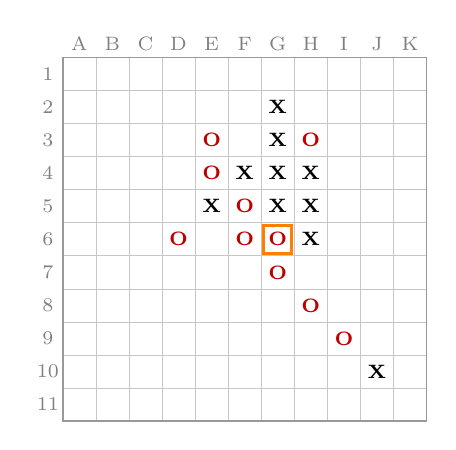
\begin{tikzpicture}[x=.42cm, y=.42cm]
\draw[gray!45, line width=.25pt] (0,0) -- (11,0);
\draw[gray!45, line width=.25pt] (0,0) -- (0,-11);
\draw[gray!45, line width=.25pt] (0,-1) -- (11,-1);
\draw[gray!45, line width=.25pt] (1,0) -- (1,-11);
\draw[gray!45, line width=.25pt] (0,-2) -- (11,-2);
\draw[gray!45, line width=.25pt] (2,0) -- (2,-11);
\draw[gray!45, line width=.25pt] (0,-3) -- (11,-3);
\draw[gray!45, line width=.25pt] (3,0) -- (3,-11);
\draw[gray!45, line width=.25pt] (0,-4) -- (11,-4);
\draw[gray!45, line width=.25pt] (4,0) -- (4,-11);
\draw[gray!45, line width=.25pt] (0,-5) -- (11,-5);
\draw[gray!45, line width=.25pt] (5,0) -- (5,-11);
\draw[gray!45, line width=.25pt] (0,-6) -- (11,-6);
\draw[gray!45, line width=.25pt] (6,0) -- (6,-11);
\draw[gray!45, line width=.25pt] (0,-7) -- (11,-7);
\draw[gray!45, line width=.25pt] (7,0) -- (7,-11);
\draw[gray!45, line width=.25pt] (0,-8) -- (11,-8);
\draw[gray!45, line width=.25pt] (8,0) -- (8,-11);
\draw[gray!45, line width=.25pt] (0,-9) -- (11,-9);
\draw[gray!45, line width=.25pt] (9,0) -- (9,-11);
\draw[gray!45, line width=.25pt] (0,-10) -- (11,-10);
\draw[gray!45, line width=.25pt] (10,0) -- (10,-11);
\draw[gray!45, line width=.25pt] (0,-11) -- (11,-11);
\draw[gray!45, line width=.25pt] (11,0) -- (11,-11);
\draw[gray!80, line width=.5pt] (0,0) rectangle (11,-11);
\node[font=\scriptsize, text=gray] at (0.5,.42) {A};
\node[font=\scriptsize, text=gray] at (1.5,.42) {B};
\node[font=\scriptsize, text=gray] at (2.5,.42) {C};
\node[font=\scriptsize, text=gray] at (3.5,.42) {D};
\node[font=\scriptsize, text=gray] at (4.5,.42) {E};
\node[font=\scriptsize, text=gray] at (5.5,.42) {F};
\node[font=\scriptsize, text=gray] at (6.5,.42) {G};
\node[font=\scriptsize, text=gray] at (7.5,.42) {H};
\node[font=\scriptsize, text=gray] at (8.5,.42) {I};
\node[font=\scriptsize, text=gray] at (9.5,.42) {J};
\node[font=\scriptsize, text=gray] at (10.5,.42) {K};
\node[font=\scriptsize, text=gray] at (-.45,-0.5) {1};
\node[font=\scriptsize, text=gray] at (-.45,-1.5) {2};
\node[font=\scriptsize, text=gray] at (-.45,-2.5) {3};
\node[font=\scriptsize, text=gray] at (-.45,-3.5) {4};
\node[font=\scriptsize, text=gray] at (-.45,-4.5) {5};
\node[font=\scriptsize, text=gray] at (-.45,-5.5) {6};
\node[font=\scriptsize, text=gray] at (-.45,-6.5) {7};
\node[font=\scriptsize, text=gray] at (-.45,-7.5) {8};
\node[font=\scriptsize, text=gray] at (-.45,-8.5) {9};
\node[font=\scriptsize, text=gray] at (-.45,-9.5) {10};
\node[font=\scriptsize, text=gray] at (-.45,-10.5) {11};
\node[text=black, font=\bfseries\scriptsize] at (6.5,-1.5) {X};
\node[text=red!75!black, font=\bfseries\scriptsize] at (4.5,-2.5) {O};
\node[text=black, font=\bfseries\scriptsize] at (6.5,-2.5) {X};
\node[text=red!75!black, font=\bfseries\scriptsize] at (7.5,-2.5) {O};
\node[text=red!75!black, font=\bfseries\scriptsize] at (4.5,-3.5) {O};
\node[text=black, font=\bfseries\scriptsize] at (5.5,-3.5) {X};
\node[text=black, font=\bfseries\scriptsize] at (6.5,-3.5) {X};
\node[text=black, font=\bfseries\scriptsize] at (7.5,-3.5) {X};
\node[text=black, font=\bfseries\scriptsize] at (4.5,-4.5) {X};
\node[text=red!75!black, font=\bfseries\scriptsize] at (5.5,-4.5) {O};
\node[text=black, font=\bfseries\scriptsize] at (6.5,-4.5) {X};
\node[text=black, font=\bfseries\scriptsize] at (7.5,-4.5) {X};
\node[text=red!75!black, font=\bfseries\scriptsize] at (3.5,-5.5) {O};
\node[text=red!75!black, font=\bfseries\scriptsize] at (5.5,-5.5) {O};
\node[text=red!75!black, font=\bfseries\scriptsize] at (6.5,-5.5) {O};
\draw[orange, line width=1pt] (6.08,-5.08) rectangle ++(.84,-.84);
\node[text=black, font=\bfseries\scriptsize] at (7.5,-5.5) {X};
\node[text=red!75!black, font=\bfseries\scriptsize] at (6.5,-6.5) {O};
\node[text=red!75!black, font=\bfseries\scriptsize] at (7.5,-7.5) {O};
\node[text=red!75!black, font=\bfseries\scriptsize] at (8.5,-8.5) {O};
\node[text=black, font=\bfseries\scriptsize] at (9.5,-9.5) {X};
\end{tikzpicture}
\end{center}
\paragraph{Thế kết thúc}
\begin{center}
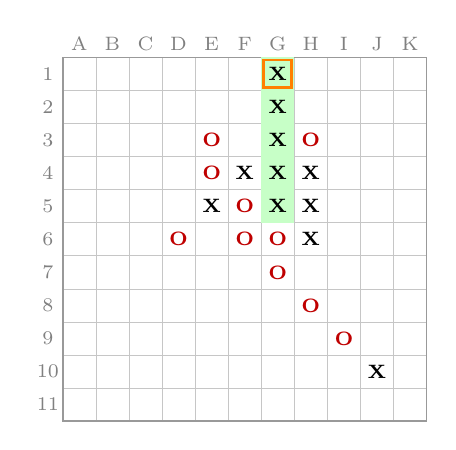
\begin{tikzpicture}[x=.42cm, y=.42cm]
\draw[gray!45, line width=.25pt] (0,0) -- (11,0);
\draw[gray!45, line width=.25pt] (0,0) -- (0,-11);
\draw[gray!45, line width=.25pt] (0,-1) -- (11,-1);
\draw[gray!45, line width=.25pt] (1,0) -- (1,-11);
\draw[gray!45, line width=.25pt] (0,-2) -- (11,-2);
\draw[gray!45, line width=.25pt] (2,0) -- (2,-11);
\draw[gray!45, line width=.25pt] (0,-3) -- (11,-3);
\draw[gray!45, line width=.25pt] (3,0) -- (3,-11);
\draw[gray!45, line width=.25pt] (0,-4) -- (11,-4);
\draw[gray!45, line width=.25pt] (4,0) -- (4,-11);
\draw[gray!45, line width=.25pt] (0,-5) -- (11,-5);
\draw[gray!45, line width=.25pt] (5,0) -- (5,-11);
\draw[gray!45, line width=.25pt] (0,-6) -- (11,-6);
\draw[gray!45, line width=.25pt] (6,0) -- (6,-11);
\draw[gray!45, line width=.25pt] (0,-7) -- (11,-7);
\draw[gray!45, line width=.25pt] (7,0) -- (7,-11);
\draw[gray!45, line width=.25pt] (0,-8) -- (11,-8);
\draw[gray!45, line width=.25pt] (8,0) -- (8,-11);
\draw[gray!45, line width=.25pt] (0,-9) -- (11,-9);
\draw[gray!45, line width=.25pt] (9,0) -- (9,-11);
\draw[gray!45, line width=.25pt] (0,-10) -- (11,-10);
\draw[gray!45, line width=.25pt] (10,0) -- (10,-11);
\draw[gray!45, line width=.25pt] (0,-11) -- (11,-11);
\draw[gray!45, line width=.25pt] (11,0) -- (11,-11);
\draw[gray!80, line width=.5pt] (0,0) rectangle (11,-11);
\node[font=\scriptsize, text=gray] at (0.5,.42) {A};
\node[font=\scriptsize, text=gray] at (1.5,.42) {B};
\node[font=\scriptsize, text=gray] at (2.5,.42) {C};
\node[font=\scriptsize, text=gray] at (3.5,.42) {D};
\node[font=\scriptsize, text=gray] at (4.5,.42) {E};
\node[font=\scriptsize, text=gray] at (5.5,.42) {F};
\node[font=\scriptsize, text=gray] at (6.5,.42) {G};
\node[font=\scriptsize, text=gray] at (7.5,.42) {H};
\node[font=\scriptsize, text=gray] at (8.5,.42) {I};
\node[font=\scriptsize, text=gray] at (9.5,.42) {J};
\node[font=\scriptsize, text=gray] at (10.5,.42) {K};
\node[font=\scriptsize, text=gray] at (-.45,-0.5) {1};
\node[font=\scriptsize, text=gray] at (-.45,-1.5) {2};
\node[font=\scriptsize, text=gray] at (-.45,-2.5) {3};
\node[font=\scriptsize, text=gray] at (-.45,-3.5) {4};
\node[font=\scriptsize, text=gray] at (-.45,-4.5) {5};
\node[font=\scriptsize, text=gray] at (-.45,-5.5) {6};
\node[font=\scriptsize, text=gray] at (-.45,-6.5) {7};
\node[font=\scriptsize, text=gray] at (-.45,-7.5) {8};
\node[font=\scriptsize, text=gray] at (-.45,-8.5) {9};
\node[font=\scriptsize, text=gray] at (-.45,-9.5) {10};
\node[font=\scriptsize, text=gray] at (-.45,-10.5) {11};
\fill[green!22] (6,0) rectangle ++(1,-1);
\node[text=black, font=\bfseries\scriptsize] at (6.5,-0.5) {X};
\draw[orange, line width=1pt] (6.08,-0.08) rectangle ++(.84,-.84);
\fill[green!22] (6,-1) rectangle ++(1,-1);
\node[text=black, font=\bfseries\scriptsize] at (6.5,-1.5) {X};
\node[text=red!75!black, font=\bfseries\scriptsize] at (4.5,-2.5) {O};
\fill[green!22] (6,-2) rectangle ++(1,-1);
\node[text=black, font=\bfseries\scriptsize] at (6.5,-2.5) {X};
\node[text=red!75!black, font=\bfseries\scriptsize] at (7.5,-2.5) {O};
\node[text=red!75!black, font=\bfseries\scriptsize] at (4.5,-3.5) {O};
\node[text=black, font=\bfseries\scriptsize] at (5.5,-3.5) {X};
\fill[green!22] (6,-3) rectangle ++(1,-1);
\node[text=black, font=\bfseries\scriptsize] at (6.5,-3.5) {X};
\node[text=black, font=\bfseries\scriptsize] at (7.5,-3.5) {X};
\node[text=black, font=\bfseries\scriptsize] at (4.5,-4.5) {X};
\node[text=red!75!black, font=\bfseries\scriptsize] at (5.5,-4.5) {O};
\fill[green!22] (6,-4) rectangle ++(1,-1);
\node[text=black, font=\bfseries\scriptsize] at (6.5,-4.5) {X};
\node[text=black, font=\bfseries\scriptsize] at (7.5,-4.5) {X};
\node[text=red!75!black, font=\bfseries\scriptsize] at (3.5,-5.5) {O};
\node[text=red!75!black, font=\bfseries\scriptsize] at (5.5,-5.5) {O};
\node[text=red!75!black, font=\bfseries\scriptsize] at (6.5,-5.5) {O};
\node[text=black, font=\bfseries\scriptsize] at (7.5,-5.5) {X};
\node[text=red!75!black, font=\bfseries\scriptsize] at (6.5,-6.5) {O};
\node[text=red!75!black, font=\bfseries\scriptsize] at (7.5,-7.5) {O};
\node[text=red!75!black, font=\bfseries\scriptsize] at (8.5,-8.5) {O};
\node[text=black, font=\bfseries\scriptsize] at (9.5,-9.5) {X};
\end{tikzpicture}
\end{center}
\paragraph{Cơ chế kết thúc} Trước nước áp chót, bên thắng đã có 2 ô thắng ngay (G1, G6); đối thủ chỉ chặn được một ô, nên nước G1 hoàn thành dãy năm quân.
\paragraph{Nhận xét} L8 cầm X xây dựng cột G từ G5 xuống G1. Đến nước 20, X đã có bốn quân G2–G5; hai đầu G1 và G6 đều là ô thắng. O chặn G6, X đi G1 và thắng. Đây là đòn kép hai đầu kinh điển: không phải O bỏ sót một ô chặn duy nhất, mà O bị buộc phải chọn giữa hai ô. Ván cho thấy L8 biết biến lợi thế trung tâm thành đe doạ dọc.
\paragraph{Diễn biến} {\footnotesize 1.H5 2.G7 3.G5 4.F6 5.E5 6.F5 7.F4 8.H8 9.H6 10.E3 11.H4 12.H3 13.G4 14.I9 15.J10 16.E4 17.G3 18.D6 19.G2 20.G6 21.G1\par}

\subsection{L8–L3 · ván 04}
Khai cuộc gồm 3 nước: E5 → G8 → H8. X: \texttt{L8-AlphaZero}, O: \texttt{L3-AlphaBeta}. Kết quả: O thắng sau 54 nước.
\begin{center}\small
\begin{tabular}{@{}rccll@{}}
\toprule
Ply & Màu & Nước & Nhận xét & Ô liên quan \\
\midrule
15 & X & G6 & Chặn bắt buộc & G6 \\
21 & X & K4 & Chặn bắt buộc & K4 \\
23 & X & I10 & Chặn bắt buộc & I10 \\
29 & X & D2 & Chặn bắt buộc & D2 \\
34 & O & D8 & Chặn bắt buộc & D8 \\
53 & X & G10 & Bỏ chặn duy nhất & D3 \\
\bottomrule
\end{tabular}
\end{center}
\paragraph{Thế cờ trước nước quyết định (sau nước 52)}
\begin{center}
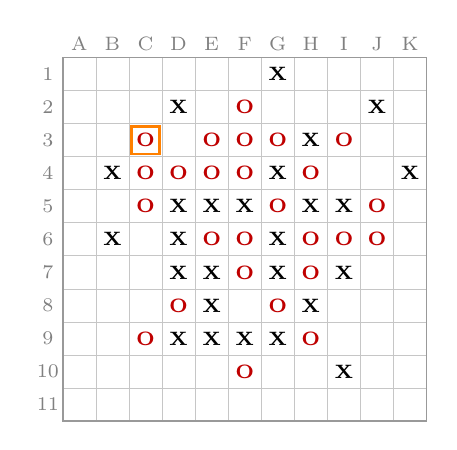
\begin{tikzpicture}[x=.42cm, y=.42cm]
\draw[gray!45, line width=.25pt] (0,0) -- (11,0);
\draw[gray!45, line width=.25pt] (0,0) -- (0,-11);
\draw[gray!45, line width=.25pt] (0,-1) -- (11,-1);
\draw[gray!45, line width=.25pt] (1,0) -- (1,-11);
\draw[gray!45, line width=.25pt] (0,-2) -- (11,-2);
\draw[gray!45, line width=.25pt] (2,0) -- (2,-11);
\draw[gray!45, line width=.25pt] (0,-3) -- (11,-3);
\draw[gray!45, line width=.25pt] (3,0) -- (3,-11);
\draw[gray!45, line width=.25pt] (0,-4) -- (11,-4);
\draw[gray!45, line width=.25pt] (4,0) -- (4,-11);
\draw[gray!45, line width=.25pt] (0,-5) -- (11,-5);
\draw[gray!45, line width=.25pt] (5,0) -- (5,-11);
\draw[gray!45, line width=.25pt] (0,-6) -- (11,-6);
\draw[gray!45, line width=.25pt] (6,0) -- (6,-11);
\draw[gray!45, line width=.25pt] (0,-7) -- (11,-7);
\draw[gray!45, line width=.25pt] (7,0) -- (7,-11);
\draw[gray!45, line width=.25pt] (0,-8) -- (11,-8);
\draw[gray!45, line width=.25pt] (8,0) -- (8,-11);
\draw[gray!45, line width=.25pt] (0,-9) -- (11,-9);
\draw[gray!45, line width=.25pt] (9,0) -- (9,-11);
\draw[gray!45, line width=.25pt] (0,-10) -- (11,-10);
\draw[gray!45, line width=.25pt] (10,0) -- (10,-11);
\draw[gray!45, line width=.25pt] (0,-11) -- (11,-11);
\draw[gray!45, line width=.25pt] (11,0) -- (11,-11);
\draw[gray!80, line width=.5pt] (0,0) rectangle (11,-11);
\node[font=\scriptsize, text=gray] at (0.5,.42) {A};
\node[font=\scriptsize, text=gray] at (1.5,.42) {B};
\node[font=\scriptsize, text=gray] at (2.5,.42) {C};
\node[font=\scriptsize, text=gray] at (3.5,.42) {D};
\node[font=\scriptsize, text=gray] at (4.5,.42) {E};
\node[font=\scriptsize, text=gray] at (5.5,.42) {F};
\node[font=\scriptsize, text=gray] at (6.5,.42) {G};
\node[font=\scriptsize, text=gray] at (7.5,.42) {H};
\node[font=\scriptsize, text=gray] at (8.5,.42) {I};
\node[font=\scriptsize, text=gray] at (9.5,.42) {J};
\node[font=\scriptsize, text=gray] at (10.5,.42) {K};
\node[font=\scriptsize, text=gray] at (-.45,-0.5) {1};
\node[font=\scriptsize, text=gray] at (-.45,-1.5) {2};
\node[font=\scriptsize, text=gray] at (-.45,-2.5) {3};
\node[font=\scriptsize, text=gray] at (-.45,-3.5) {4};
\node[font=\scriptsize, text=gray] at (-.45,-4.5) {5};
\node[font=\scriptsize, text=gray] at (-.45,-5.5) {6};
\node[font=\scriptsize, text=gray] at (-.45,-6.5) {7};
\node[font=\scriptsize, text=gray] at (-.45,-7.5) {8};
\node[font=\scriptsize, text=gray] at (-.45,-8.5) {9};
\node[font=\scriptsize, text=gray] at (-.45,-9.5) {10};
\node[font=\scriptsize, text=gray] at (-.45,-10.5) {11};
\node[text=black, font=\bfseries\scriptsize] at (6.5,-0.5) {X};
\node[text=black, font=\bfseries\scriptsize] at (3.5,-1.5) {X};
\node[text=red!75!black, font=\bfseries\scriptsize] at (5.5,-1.5) {O};
\node[text=black, font=\bfseries\scriptsize] at (9.5,-1.5) {X};
\node[text=red!75!black, font=\bfseries\scriptsize] at (2.5,-2.5) {O};
\draw[orange, line width=1pt] (2.08,-2.08) rectangle ++(.84,-.84);
\node[text=red!75!black, font=\bfseries\scriptsize] at (4.5,-2.5) {O};
\node[text=red!75!black, font=\bfseries\scriptsize] at (5.5,-2.5) {O};
\node[text=red!75!black, font=\bfseries\scriptsize] at (6.5,-2.5) {O};
\node[text=black, font=\bfseries\scriptsize] at (7.5,-2.5) {X};
\node[text=red!75!black, font=\bfseries\scriptsize] at (8.5,-2.5) {O};
\node[text=black, font=\bfseries\scriptsize] at (1.5,-3.5) {X};
\node[text=red!75!black, font=\bfseries\scriptsize] at (2.5,-3.5) {O};
\node[text=red!75!black, font=\bfseries\scriptsize] at (3.5,-3.5) {O};
\node[text=red!75!black, font=\bfseries\scriptsize] at (4.5,-3.5) {O};
\node[text=red!75!black, font=\bfseries\scriptsize] at (5.5,-3.5) {O};
\node[text=black, font=\bfseries\scriptsize] at (6.5,-3.5) {X};
\node[text=red!75!black, font=\bfseries\scriptsize] at (7.5,-3.5) {O};
\node[text=black, font=\bfseries\scriptsize] at (10.5,-3.5) {X};
\node[text=red!75!black, font=\bfseries\scriptsize] at (2.5,-4.5) {O};
\node[text=black, font=\bfseries\scriptsize] at (3.5,-4.5) {X};
\node[text=black, font=\bfseries\scriptsize] at (4.5,-4.5) {X};
\node[text=black, font=\bfseries\scriptsize] at (5.5,-4.5) {X};
\node[text=red!75!black, font=\bfseries\scriptsize] at (6.5,-4.5) {O};
\node[text=black, font=\bfseries\scriptsize] at (7.5,-4.5) {X};
\node[text=black, font=\bfseries\scriptsize] at (8.5,-4.5) {X};
\node[text=red!75!black, font=\bfseries\scriptsize] at (9.5,-4.5) {O};
\node[text=black, font=\bfseries\scriptsize] at (1.5,-5.5) {X};
\node[text=black, font=\bfseries\scriptsize] at (3.5,-5.5) {X};
\node[text=red!75!black, font=\bfseries\scriptsize] at (4.5,-5.5) {O};
\node[text=red!75!black, font=\bfseries\scriptsize] at (5.5,-5.5) {O};
\node[text=black, font=\bfseries\scriptsize] at (6.5,-5.5) {X};
\node[text=red!75!black, font=\bfseries\scriptsize] at (7.5,-5.5) {O};
\node[text=red!75!black, font=\bfseries\scriptsize] at (8.5,-5.5) {O};
\node[text=red!75!black, font=\bfseries\scriptsize] at (9.5,-5.5) {O};
\node[text=black, font=\bfseries\scriptsize] at (3.5,-6.5) {X};
\node[text=black, font=\bfseries\scriptsize] at (4.5,-6.5) {X};
\node[text=red!75!black, font=\bfseries\scriptsize] at (5.5,-6.5) {O};
\node[text=black, font=\bfseries\scriptsize] at (6.5,-6.5) {X};
\node[text=red!75!black, font=\bfseries\scriptsize] at (7.5,-6.5) {O};
\node[text=black, font=\bfseries\scriptsize] at (8.5,-6.5) {X};
\node[text=red!75!black, font=\bfseries\scriptsize] at (3.5,-7.5) {O};
\node[text=black, font=\bfseries\scriptsize] at (4.5,-7.5) {X};
\node[text=red!75!black, font=\bfseries\scriptsize] at (6.5,-7.5) {O};
\node[text=black, font=\bfseries\scriptsize] at (7.5,-7.5) {X};
\node[text=red!75!black, font=\bfseries\scriptsize] at (2.5,-8.5) {O};
\node[text=black, font=\bfseries\scriptsize] at (3.5,-8.5) {X};
\node[text=black, font=\bfseries\scriptsize] at (4.5,-8.5) {X};
\node[text=black, font=\bfseries\scriptsize] at (5.5,-8.5) {X};
\node[text=black, font=\bfseries\scriptsize] at (6.5,-8.5) {X};
\node[text=red!75!black, font=\bfseries\scriptsize] at (7.5,-8.5) {O};
\node[text=red!75!black, font=\bfseries\scriptsize] at (5.5,-9.5) {O};
\node[text=black, font=\bfseries\scriptsize] at (8.5,-9.5) {X};
\end{tikzpicture}
\end{center}
\paragraph{Thế kết thúc}
\begin{center}
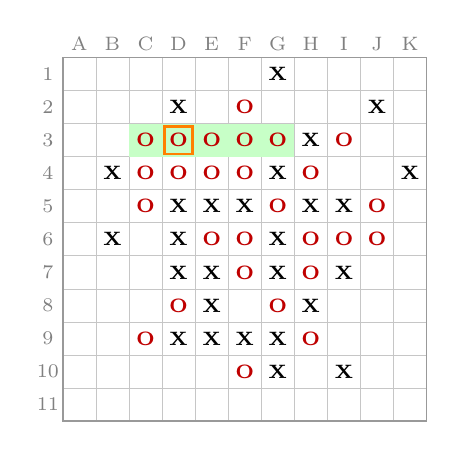
\begin{tikzpicture}[x=.42cm, y=.42cm]
\draw[gray!45, line width=.25pt] (0,0) -- (11,0);
\draw[gray!45, line width=.25pt] (0,0) -- (0,-11);
\draw[gray!45, line width=.25pt] (0,-1) -- (11,-1);
\draw[gray!45, line width=.25pt] (1,0) -- (1,-11);
\draw[gray!45, line width=.25pt] (0,-2) -- (11,-2);
\draw[gray!45, line width=.25pt] (2,0) -- (2,-11);
\draw[gray!45, line width=.25pt] (0,-3) -- (11,-3);
\draw[gray!45, line width=.25pt] (3,0) -- (3,-11);
\draw[gray!45, line width=.25pt] (0,-4) -- (11,-4);
\draw[gray!45, line width=.25pt] (4,0) -- (4,-11);
\draw[gray!45, line width=.25pt] (0,-5) -- (11,-5);
\draw[gray!45, line width=.25pt] (5,0) -- (5,-11);
\draw[gray!45, line width=.25pt] (0,-6) -- (11,-6);
\draw[gray!45, line width=.25pt] (6,0) -- (6,-11);
\draw[gray!45, line width=.25pt] (0,-7) -- (11,-7);
\draw[gray!45, line width=.25pt] (7,0) -- (7,-11);
\draw[gray!45, line width=.25pt] (0,-8) -- (11,-8);
\draw[gray!45, line width=.25pt] (8,0) -- (8,-11);
\draw[gray!45, line width=.25pt] (0,-9) -- (11,-9);
\draw[gray!45, line width=.25pt] (9,0) -- (9,-11);
\draw[gray!45, line width=.25pt] (0,-10) -- (11,-10);
\draw[gray!45, line width=.25pt] (10,0) -- (10,-11);
\draw[gray!45, line width=.25pt] (0,-11) -- (11,-11);
\draw[gray!45, line width=.25pt] (11,0) -- (11,-11);
\draw[gray!80, line width=.5pt] (0,0) rectangle (11,-11);
\node[font=\scriptsize, text=gray] at (0.5,.42) {A};
\node[font=\scriptsize, text=gray] at (1.5,.42) {B};
\node[font=\scriptsize, text=gray] at (2.5,.42) {C};
\node[font=\scriptsize, text=gray] at (3.5,.42) {D};
\node[font=\scriptsize, text=gray] at (4.5,.42) {E};
\node[font=\scriptsize, text=gray] at (5.5,.42) {F};
\node[font=\scriptsize, text=gray] at (6.5,.42) {G};
\node[font=\scriptsize, text=gray] at (7.5,.42) {H};
\node[font=\scriptsize, text=gray] at (8.5,.42) {I};
\node[font=\scriptsize, text=gray] at (9.5,.42) {J};
\node[font=\scriptsize, text=gray] at (10.5,.42) {K};
\node[font=\scriptsize, text=gray] at (-.45,-0.5) {1};
\node[font=\scriptsize, text=gray] at (-.45,-1.5) {2};
\node[font=\scriptsize, text=gray] at (-.45,-2.5) {3};
\node[font=\scriptsize, text=gray] at (-.45,-3.5) {4};
\node[font=\scriptsize, text=gray] at (-.45,-4.5) {5};
\node[font=\scriptsize, text=gray] at (-.45,-5.5) {6};
\node[font=\scriptsize, text=gray] at (-.45,-6.5) {7};
\node[font=\scriptsize, text=gray] at (-.45,-7.5) {8};
\node[font=\scriptsize, text=gray] at (-.45,-8.5) {9};
\node[font=\scriptsize, text=gray] at (-.45,-9.5) {10};
\node[font=\scriptsize, text=gray] at (-.45,-10.5) {11};
\node[text=black, font=\bfseries\scriptsize] at (6.5,-0.5) {X};
\node[text=black, font=\bfseries\scriptsize] at (3.5,-1.5) {X};
\node[text=red!75!black, font=\bfseries\scriptsize] at (5.5,-1.5) {O};
\node[text=black, font=\bfseries\scriptsize] at (9.5,-1.5) {X};
\fill[green!22] (2,-2) rectangle ++(1,-1);
\node[text=red!75!black, font=\bfseries\scriptsize] at (2.5,-2.5) {O};
\fill[green!22] (3,-2) rectangle ++(1,-1);
\node[text=red!75!black, font=\bfseries\scriptsize] at (3.5,-2.5) {O};
\draw[orange, line width=1pt] (3.08,-2.08) rectangle ++(.84,-.84);
\fill[green!22] (4,-2) rectangle ++(1,-1);
\node[text=red!75!black, font=\bfseries\scriptsize] at (4.5,-2.5) {O};
\fill[green!22] (5,-2) rectangle ++(1,-1);
\node[text=red!75!black, font=\bfseries\scriptsize] at (5.5,-2.5) {O};
\fill[green!22] (6,-2) rectangle ++(1,-1);
\node[text=red!75!black, font=\bfseries\scriptsize] at (6.5,-2.5) {O};
\node[text=black, font=\bfseries\scriptsize] at (7.5,-2.5) {X};
\node[text=red!75!black, font=\bfseries\scriptsize] at (8.5,-2.5) {O};
\node[text=black, font=\bfseries\scriptsize] at (1.5,-3.5) {X};
\node[text=red!75!black, font=\bfseries\scriptsize] at (2.5,-3.5) {O};
\node[text=red!75!black, font=\bfseries\scriptsize] at (3.5,-3.5) {O};
\node[text=red!75!black, font=\bfseries\scriptsize] at (4.5,-3.5) {O};
\node[text=red!75!black, font=\bfseries\scriptsize] at (5.5,-3.5) {O};
\node[text=black, font=\bfseries\scriptsize] at (6.5,-3.5) {X};
\node[text=red!75!black, font=\bfseries\scriptsize] at (7.5,-3.5) {O};
\node[text=black, font=\bfseries\scriptsize] at (10.5,-3.5) {X};
\node[text=red!75!black, font=\bfseries\scriptsize] at (2.5,-4.5) {O};
\node[text=black, font=\bfseries\scriptsize] at (3.5,-4.5) {X};
\node[text=black, font=\bfseries\scriptsize] at (4.5,-4.5) {X};
\node[text=black, font=\bfseries\scriptsize] at (5.5,-4.5) {X};
\node[text=red!75!black, font=\bfseries\scriptsize] at (6.5,-4.5) {O};
\node[text=black, font=\bfseries\scriptsize] at (7.5,-4.5) {X};
\node[text=black, font=\bfseries\scriptsize] at (8.5,-4.5) {X};
\node[text=red!75!black, font=\bfseries\scriptsize] at (9.5,-4.5) {O};
\node[text=black, font=\bfseries\scriptsize] at (1.5,-5.5) {X};
\node[text=black, font=\bfseries\scriptsize] at (3.5,-5.5) {X};
\node[text=red!75!black, font=\bfseries\scriptsize] at (4.5,-5.5) {O};
\node[text=red!75!black, font=\bfseries\scriptsize] at (5.5,-5.5) {O};
\node[text=black, font=\bfseries\scriptsize] at (6.5,-5.5) {X};
\node[text=red!75!black, font=\bfseries\scriptsize] at (7.5,-5.5) {O};
\node[text=red!75!black, font=\bfseries\scriptsize] at (8.5,-5.5) {O};
\node[text=red!75!black, font=\bfseries\scriptsize] at (9.5,-5.5) {O};
\node[text=black, font=\bfseries\scriptsize] at (3.5,-6.5) {X};
\node[text=black, font=\bfseries\scriptsize] at (4.5,-6.5) {X};
\node[text=red!75!black, font=\bfseries\scriptsize] at (5.5,-6.5) {O};
\node[text=black, font=\bfseries\scriptsize] at (6.5,-6.5) {X};
\node[text=red!75!black, font=\bfseries\scriptsize] at (7.5,-6.5) {O};
\node[text=black, font=\bfseries\scriptsize] at (8.5,-6.5) {X};
\node[text=red!75!black, font=\bfseries\scriptsize] at (3.5,-7.5) {O};
\node[text=black, font=\bfseries\scriptsize] at (4.5,-7.5) {X};
\node[text=red!75!black, font=\bfseries\scriptsize] at (6.5,-7.5) {O};
\node[text=black, font=\bfseries\scriptsize] at (7.5,-7.5) {X};
\node[text=red!75!black, font=\bfseries\scriptsize] at (2.5,-8.5) {O};
\node[text=black, font=\bfseries\scriptsize] at (3.5,-8.5) {X};
\node[text=black, font=\bfseries\scriptsize] at (4.5,-8.5) {X};
\node[text=black, font=\bfseries\scriptsize] at (5.5,-8.5) {X};
\node[text=black, font=\bfseries\scriptsize] at (6.5,-8.5) {X};
\node[text=red!75!black, font=\bfseries\scriptsize] at (7.5,-8.5) {O};
\node[text=red!75!black, font=\bfseries\scriptsize] at (5.5,-9.5) {O};
\node[text=black, font=\bfseries\scriptsize] at (6.5,-9.5) {X};
\node[text=black, font=\bfseries\scriptsize] at (8.5,-9.5) {X};
\end{tikzpicture}
\end{center}
\paragraph{Cơ chế kết thúc} Trước nước áp chót, bên thắng có đúng một ô thắng ngay (D3); đối thủ không chặn, nên nước D3 hoàn thành dãy.
\paragraph{Nhận xét} Ván dài 54 nước, L8 cầm X thua. Ở nước 53, O đã có bốn quân C3, E3, F3, G3; D3 là ô thắng duy nhất. X đi G10 thay vì chặn D3, O đi D3 và hoàn thành hàng ngang C3–G3. Đây là lỗi chiến thuật rõ ràng duy nhất trong ván: trước đó hai bên đổi đe doạ ở nhiều cánh, nhưng đến nước 53 chỉ còn một nước cứu. L8 với 200 mô phỏng vẫn có thể bỏ sót nước bắt buộc khi cây tìm kiếm bị phân tán.
\paragraph{Diễn biến} {\footnotesize 1.E5 2.G8 3.H8 4.H7 5.F5 6.G5 7.G7 8.F6 9.E7 10.I6 11.F9 12.E6 13.D6 14.H6 15.G6 16.F4 17.I7 18.F7 19.D5 20.J5 21.K4 22.H9 23.I10 24.C5 25.G9 26.F10 27.D7 28.E3 29.D2 30.D4 31.B6 32.H4 33.D9 34.D8 35.E9 36.C9 37.H5 38.E4 39.G4 40.J6 41.E8 42.F2 43.G1 44.I3 45.J2 46.G3 47.I5 48.C4 49.B4 50.F3 51.H3 52.C3 53.G10 54.D3\par}

\subsection{L3–L8 · ván 24}
Khai cuộc gồm 3 nước: E5 → G8 → H8. X: \texttt{L3-AlphaBeta}, O: \texttt{L8-AlphaZero}. Kết quả: O thắng sau 26 nước.
\begin{center}\small
\begin{tabular}{@{}rccll@{}}
\toprule
Ply & Màu & Nước & Nhận xét & Ô liên quan \\
\midrule
17 & X & D11 & Chặn bắt buộc & D11 \\
20 & O & D5 & Chặn bắt buộc & D5 \\
25 & X & D6 & Đã ở thế buộc thua & — \\
26 & O & I11 & Thắng ngay & — \\
\bottomrule
\end{tabular}
\end{center}
\paragraph{Thế cờ trước nước quyết định (sau nước 25)}
\begin{center}
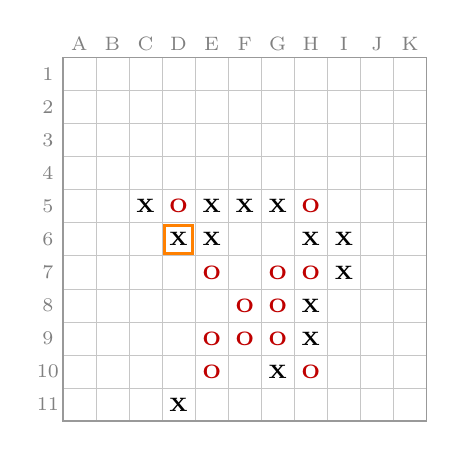
\begin{tikzpicture}[x=.42cm, y=.42cm]
\draw[gray!45, line width=.25pt] (0,0) -- (11,0);
\draw[gray!45, line width=.25pt] (0,0) -- (0,-11);
\draw[gray!45, line width=.25pt] (0,-1) -- (11,-1);
\draw[gray!45, line width=.25pt] (1,0) -- (1,-11);
\draw[gray!45, line width=.25pt] (0,-2) -- (11,-2);
\draw[gray!45, line width=.25pt] (2,0) -- (2,-11);
\draw[gray!45, line width=.25pt] (0,-3) -- (11,-3);
\draw[gray!45, line width=.25pt] (3,0) -- (3,-11);
\draw[gray!45, line width=.25pt] (0,-4) -- (11,-4);
\draw[gray!45, line width=.25pt] (4,0) -- (4,-11);
\draw[gray!45, line width=.25pt] (0,-5) -- (11,-5);
\draw[gray!45, line width=.25pt] (5,0) -- (5,-11);
\draw[gray!45, line width=.25pt] (0,-6) -- (11,-6);
\draw[gray!45, line width=.25pt] (6,0) -- (6,-11);
\draw[gray!45, line width=.25pt] (0,-7) -- (11,-7);
\draw[gray!45, line width=.25pt] (7,0) -- (7,-11);
\draw[gray!45, line width=.25pt] (0,-8) -- (11,-8);
\draw[gray!45, line width=.25pt] (8,0) -- (8,-11);
\draw[gray!45, line width=.25pt] (0,-9) -- (11,-9);
\draw[gray!45, line width=.25pt] (9,0) -- (9,-11);
\draw[gray!45, line width=.25pt] (0,-10) -- (11,-10);
\draw[gray!45, line width=.25pt] (10,0) -- (10,-11);
\draw[gray!45, line width=.25pt] (0,-11) -- (11,-11);
\draw[gray!45, line width=.25pt] (11,0) -- (11,-11);
\draw[gray!80, line width=.5pt] (0,0) rectangle (11,-11);
\node[font=\scriptsize, text=gray] at (0.5,.42) {A};
\node[font=\scriptsize, text=gray] at (1.5,.42) {B};
\node[font=\scriptsize, text=gray] at (2.5,.42) {C};
\node[font=\scriptsize, text=gray] at (3.5,.42) {D};
\node[font=\scriptsize, text=gray] at (4.5,.42) {E};
\node[font=\scriptsize, text=gray] at (5.5,.42) {F};
\node[font=\scriptsize, text=gray] at (6.5,.42) {G};
\node[font=\scriptsize, text=gray] at (7.5,.42) {H};
\node[font=\scriptsize, text=gray] at (8.5,.42) {I};
\node[font=\scriptsize, text=gray] at (9.5,.42) {J};
\node[font=\scriptsize, text=gray] at (10.5,.42) {K};
\node[font=\scriptsize, text=gray] at (-.45,-0.5) {1};
\node[font=\scriptsize, text=gray] at (-.45,-1.5) {2};
\node[font=\scriptsize, text=gray] at (-.45,-2.5) {3};
\node[font=\scriptsize, text=gray] at (-.45,-3.5) {4};
\node[font=\scriptsize, text=gray] at (-.45,-4.5) {5};
\node[font=\scriptsize, text=gray] at (-.45,-5.5) {6};
\node[font=\scriptsize, text=gray] at (-.45,-6.5) {7};
\node[font=\scriptsize, text=gray] at (-.45,-7.5) {8};
\node[font=\scriptsize, text=gray] at (-.45,-8.5) {9};
\node[font=\scriptsize, text=gray] at (-.45,-9.5) {10};
\node[font=\scriptsize, text=gray] at (-.45,-10.5) {11};
\node[text=black, font=\bfseries\scriptsize] at (2.5,-4.5) {X};
\node[text=red!75!black, font=\bfseries\scriptsize] at (3.5,-4.5) {O};
\node[text=black, font=\bfseries\scriptsize] at (4.5,-4.5) {X};
\node[text=black, font=\bfseries\scriptsize] at (5.5,-4.5) {X};
\node[text=black, font=\bfseries\scriptsize] at (6.5,-4.5) {X};
\node[text=red!75!black, font=\bfseries\scriptsize] at (7.5,-4.5) {O};
\node[text=black, font=\bfseries\scriptsize] at (3.5,-5.5) {X};
\draw[orange, line width=1pt] (3.08,-5.08) rectangle ++(.84,-.84);
\node[text=black, font=\bfseries\scriptsize] at (4.5,-5.5) {X};
\node[text=black, font=\bfseries\scriptsize] at (7.5,-5.5) {X};
\node[text=black, font=\bfseries\scriptsize] at (8.5,-5.5) {X};
\node[text=red!75!black, font=\bfseries\scriptsize] at (4.5,-6.5) {O};
\node[text=red!75!black, font=\bfseries\scriptsize] at (6.5,-6.5) {O};
\node[text=red!75!black, font=\bfseries\scriptsize] at (7.5,-6.5) {O};
\node[text=black, font=\bfseries\scriptsize] at (8.5,-6.5) {X};
\node[text=red!75!black, font=\bfseries\scriptsize] at (5.5,-7.5) {O};
\node[text=red!75!black, font=\bfseries\scriptsize] at (6.5,-7.5) {O};
\node[text=black, font=\bfseries\scriptsize] at (7.5,-7.5) {X};
\node[text=red!75!black, font=\bfseries\scriptsize] at (4.5,-8.5) {O};
\node[text=red!75!black, font=\bfseries\scriptsize] at (5.5,-8.5) {O};
\node[text=red!75!black, font=\bfseries\scriptsize] at (6.5,-8.5) {O};
\node[text=black, font=\bfseries\scriptsize] at (7.5,-8.5) {X};
\node[text=red!75!black, font=\bfseries\scriptsize] at (4.5,-9.5) {O};
\node[text=black, font=\bfseries\scriptsize] at (6.5,-9.5) {X};
\node[text=red!75!black, font=\bfseries\scriptsize] at (7.5,-9.5) {O};
\node[text=black, font=\bfseries\scriptsize] at (3.5,-10.5) {X};
\end{tikzpicture}
\end{center}
\paragraph{Thế kết thúc}
\begin{center}
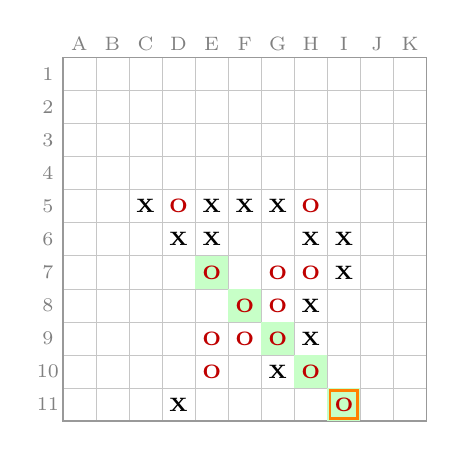
\begin{tikzpicture}[x=.42cm, y=.42cm]
\draw[gray!45, line width=.25pt] (0,0) -- (11,0);
\draw[gray!45, line width=.25pt] (0,0) -- (0,-11);
\draw[gray!45, line width=.25pt] (0,-1) -- (11,-1);
\draw[gray!45, line width=.25pt] (1,0) -- (1,-11);
\draw[gray!45, line width=.25pt] (0,-2) -- (11,-2);
\draw[gray!45, line width=.25pt] (2,0) -- (2,-11);
\draw[gray!45, line width=.25pt] (0,-3) -- (11,-3);
\draw[gray!45, line width=.25pt] (3,0) -- (3,-11);
\draw[gray!45, line width=.25pt] (0,-4) -- (11,-4);
\draw[gray!45, line width=.25pt] (4,0) -- (4,-11);
\draw[gray!45, line width=.25pt] (0,-5) -- (11,-5);
\draw[gray!45, line width=.25pt] (5,0) -- (5,-11);
\draw[gray!45, line width=.25pt] (0,-6) -- (11,-6);
\draw[gray!45, line width=.25pt] (6,0) -- (6,-11);
\draw[gray!45, line width=.25pt] (0,-7) -- (11,-7);
\draw[gray!45, line width=.25pt] (7,0) -- (7,-11);
\draw[gray!45, line width=.25pt] (0,-8) -- (11,-8);
\draw[gray!45, line width=.25pt] (8,0) -- (8,-11);
\draw[gray!45, line width=.25pt] (0,-9) -- (11,-9);
\draw[gray!45, line width=.25pt] (9,0) -- (9,-11);
\draw[gray!45, line width=.25pt] (0,-10) -- (11,-10);
\draw[gray!45, line width=.25pt] (10,0) -- (10,-11);
\draw[gray!45, line width=.25pt] (0,-11) -- (11,-11);
\draw[gray!45, line width=.25pt] (11,0) -- (11,-11);
\draw[gray!80, line width=.5pt] (0,0) rectangle (11,-11);
\node[font=\scriptsize, text=gray] at (0.5,.42) {A};
\node[font=\scriptsize, text=gray] at (1.5,.42) {B};
\node[font=\scriptsize, text=gray] at (2.5,.42) {C};
\node[font=\scriptsize, text=gray] at (3.5,.42) {D};
\node[font=\scriptsize, text=gray] at (4.5,.42) {E};
\node[font=\scriptsize, text=gray] at (5.5,.42) {F};
\node[font=\scriptsize, text=gray] at (6.5,.42) {G};
\node[font=\scriptsize, text=gray] at (7.5,.42) {H};
\node[font=\scriptsize, text=gray] at (8.5,.42) {I};
\node[font=\scriptsize, text=gray] at (9.5,.42) {J};
\node[font=\scriptsize, text=gray] at (10.5,.42) {K};
\node[font=\scriptsize, text=gray] at (-.45,-0.5) {1};
\node[font=\scriptsize, text=gray] at (-.45,-1.5) {2};
\node[font=\scriptsize, text=gray] at (-.45,-2.5) {3};
\node[font=\scriptsize, text=gray] at (-.45,-3.5) {4};
\node[font=\scriptsize, text=gray] at (-.45,-4.5) {5};
\node[font=\scriptsize, text=gray] at (-.45,-5.5) {6};
\node[font=\scriptsize, text=gray] at (-.45,-6.5) {7};
\node[font=\scriptsize, text=gray] at (-.45,-7.5) {8};
\node[font=\scriptsize, text=gray] at (-.45,-8.5) {9};
\node[font=\scriptsize, text=gray] at (-.45,-9.5) {10};
\node[font=\scriptsize, text=gray] at (-.45,-10.5) {11};
\node[text=black, font=\bfseries\scriptsize] at (2.5,-4.5) {X};
\node[text=red!75!black, font=\bfseries\scriptsize] at (3.5,-4.5) {O};
\node[text=black, font=\bfseries\scriptsize] at (4.5,-4.5) {X};
\node[text=black, font=\bfseries\scriptsize] at (5.5,-4.5) {X};
\node[text=black, font=\bfseries\scriptsize] at (6.5,-4.5) {X};
\node[text=red!75!black, font=\bfseries\scriptsize] at (7.5,-4.5) {O};
\node[text=black, font=\bfseries\scriptsize] at (3.5,-5.5) {X};
\node[text=black, font=\bfseries\scriptsize] at (4.5,-5.5) {X};
\node[text=black, font=\bfseries\scriptsize] at (7.5,-5.5) {X};
\node[text=black, font=\bfseries\scriptsize] at (8.5,-5.5) {X};
\fill[green!22] (4,-6) rectangle ++(1,-1);
\node[text=red!75!black, font=\bfseries\scriptsize] at (4.5,-6.5) {O};
\node[text=red!75!black, font=\bfseries\scriptsize] at (6.5,-6.5) {O};
\node[text=red!75!black, font=\bfseries\scriptsize] at (7.5,-6.5) {O};
\node[text=black, font=\bfseries\scriptsize] at (8.5,-6.5) {X};
\fill[green!22] (5,-7) rectangle ++(1,-1);
\node[text=red!75!black, font=\bfseries\scriptsize] at (5.5,-7.5) {O};
\node[text=red!75!black, font=\bfseries\scriptsize] at (6.5,-7.5) {O};
\node[text=black, font=\bfseries\scriptsize] at (7.5,-7.5) {X};
\node[text=red!75!black, font=\bfseries\scriptsize] at (4.5,-8.5) {O};
\node[text=red!75!black, font=\bfseries\scriptsize] at (5.5,-8.5) {O};
\fill[green!22] (6,-8) rectangle ++(1,-1);
\node[text=red!75!black, font=\bfseries\scriptsize] at (6.5,-8.5) {O};
\node[text=black, font=\bfseries\scriptsize] at (7.5,-8.5) {X};
\node[text=red!75!black, font=\bfseries\scriptsize] at (4.5,-9.5) {O};
\node[text=black, font=\bfseries\scriptsize] at (6.5,-9.5) {X};
\fill[green!22] (7,-9) rectangle ++(1,-1);
\node[text=red!75!black, font=\bfseries\scriptsize] at (7.5,-9.5) {O};
\node[text=black, font=\bfseries\scriptsize] at (3.5,-10.5) {X};
\fill[green!22] (8,-10) rectangle ++(1,-1);
\node[text=red!75!black, font=\bfseries\scriptsize] at (8.5,-10.5) {O};
\draw[orange, line width=1pt] (8.08,-10.08) rectangle ++(.84,-.84);
\end{tikzpicture}
\end{center}
\paragraph{Cơ chế kết thúc} Trước nước áp chót, bên thắng đã có 2 ô thắng ngay (D6, I11); đối thủ chỉ chặn được một ô, nên nước I11 hoàn thành dãy năm quân.
\paragraph{Nhận xét} L8 cầm O thắng trong 26 nước, một trong bảy ván O thắng trước L3. O xây dựng đường chéo E7–F8–G9–H10; trước nước 25, hai đầu D6 và I11 đều là ô thắng. X chặn D6, O đi I11 và thắng. Đây là ví dụ L8 không chỉ phòng thủ khi cầm O mà còn tạo được đòn kép chéo. So với các ván O thua nhanh, ván này cho thấy chất lượng tìm kiếm quyết định khả năng lật thế.
\paragraph{Diễn biến} {\footnotesize 1.E5 2.G8 3.H8 4.G7 5.G5 6.G9 7.G10 8.H7 9.F5 10.H5 11.I7 12.F9 13.I6 14.E9 15.H9 16.E10 17.D11 18.E7 19.C5 20.D5 21.E6 22.F8 23.H6 24.H10 25.D6 26.I11\par}

\subsection{L3–L8 · ván 26}
Khai cuộc gồm 3 nước: H5 → F8 → G7. X: \texttt{L3-AlphaBeta}, O: \texttt{L8-AlphaZero}. Kết quả: X thắng sau 21 nước.
\begin{center}\small
\begin{tabular}{@{}rccll@{}}
\toprule
Ply & Màu & Nước & Nhận xét & Ô liên quan \\
\midrule
18 & O & G3 & Chặn bắt buộc & G3 \\
20 & O & C8 & Bỏ chặn duy nhất & E7 \\
21 & X & E7 & Thắng ngay & — \\
\bottomrule
\end{tabular}
\end{center}
\paragraph{Thế cờ trước nước quyết định (sau nước 20)}
\begin{center}
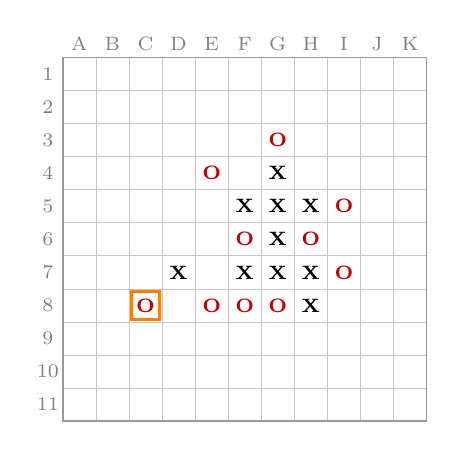
\begin{tikzpicture}[x=.42cm, y=.42cm]
\draw[gray!45, line width=.25pt] (0,0) -- (11,0);
\draw[gray!45, line width=.25pt] (0,0) -- (0,-11);
\draw[gray!45, line width=.25pt] (0,-1) -- (11,-1);
\draw[gray!45, line width=.25pt] (1,0) -- (1,-11);
\draw[gray!45, line width=.25pt] (0,-2) -- (11,-2);
\draw[gray!45, line width=.25pt] (2,0) -- (2,-11);
\draw[gray!45, line width=.25pt] (0,-3) -- (11,-3);
\draw[gray!45, line width=.25pt] (3,0) -- (3,-11);
\draw[gray!45, line width=.25pt] (0,-4) -- (11,-4);
\draw[gray!45, line width=.25pt] (4,0) -- (4,-11);
\draw[gray!45, line width=.25pt] (0,-5) -- (11,-5);
\draw[gray!45, line width=.25pt] (5,0) -- (5,-11);
\draw[gray!45, line width=.25pt] (0,-6) -- (11,-6);
\draw[gray!45, line width=.25pt] (6,0) -- (6,-11);
\draw[gray!45, line width=.25pt] (0,-7) -- (11,-7);
\draw[gray!45, line width=.25pt] (7,0) -- (7,-11);
\draw[gray!45, line width=.25pt] (0,-8) -- (11,-8);
\draw[gray!45, line width=.25pt] (8,0) -- (8,-11);
\draw[gray!45, line width=.25pt] (0,-9) -- (11,-9);
\draw[gray!45, line width=.25pt] (9,0) -- (9,-11);
\draw[gray!45, line width=.25pt] (0,-10) -- (11,-10);
\draw[gray!45, line width=.25pt] (10,0) -- (10,-11);
\draw[gray!45, line width=.25pt] (0,-11) -- (11,-11);
\draw[gray!45, line width=.25pt] (11,0) -- (11,-11);
\draw[gray!80, line width=.5pt] (0,0) rectangle (11,-11);
\node[font=\scriptsize, text=gray] at (0.5,.42) {A};
\node[font=\scriptsize, text=gray] at (1.5,.42) {B};
\node[font=\scriptsize, text=gray] at (2.5,.42) {C};
\node[font=\scriptsize, text=gray] at (3.5,.42) {D};
\node[font=\scriptsize, text=gray] at (4.5,.42) {E};
\node[font=\scriptsize, text=gray] at (5.5,.42) {F};
\node[font=\scriptsize, text=gray] at (6.5,.42) {G};
\node[font=\scriptsize, text=gray] at (7.5,.42) {H};
\node[font=\scriptsize, text=gray] at (8.5,.42) {I};
\node[font=\scriptsize, text=gray] at (9.5,.42) {J};
\node[font=\scriptsize, text=gray] at (10.5,.42) {K};
\node[font=\scriptsize, text=gray] at (-.45,-0.5) {1};
\node[font=\scriptsize, text=gray] at (-.45,-1.5) {2};
\node[font=\scriptsize, text=gray] at (-.45,-2.5) {3};
\node[font=\scriptsize, text=gray] at (-.45,-3.5) {4};
\node[font=\scriptsize, text=gray] at (-.45,-4.5) {5};
\node[font=\scriptsize, text=gray] at (-.45,-5.5) {6};
\node[font=\scriptsize, text=gray] at (-.45,-6.5) {7};
\node[font=\scriptsize, text=gray] at (-.45,-7.5) {8};
\node[font=\scriptsize, text=gray] at (-.45,-8.5) {9};
\node[font=\scriptsize, text=gray] at (-.45,-9.5) {10};
\node[font=\scriptsize, text=gray] at (-.45,-10.5) {11};
\node[text=red!75!black, font=\bfseries\scriptsize] at (6.5,-2.5) {O};
\node[text=red!75!black, font=\bfseries\scriptsize] at (4.5,-3.5) {O};
\node[text=black, font=\bfseries\scriptsize] at (6.5,-3.5) {X};
\node[text=black, font=\bfseries\scriptsize] at (5.5,-4.5) {X};
\node[text=black, font=\bfseries\scriptsize] at (6.5,-4.5) {X};
\node[text=black, font=\bfseries\scriptsize] at (7.5,-4.5) {X};
\node[text=red!75!black, font=\bfseries\scriptsize] at (8.5,-4.5) {O};
\node[text=red!75!black, font=\bfseries\scriptsize] at (5.5,-5.5) {O};
\node[text=black, font=\bfseries\scriptsize] at (6.5,-5.5) {X};
\node[text=red!75!black, font=\bfseries\scriptsize] at (7.5,-5.5) {O};
\node[text=black, font=\bfseries\scriptsize] at (3.5,-6.5) {X};
\node[text=black, font=\bfseries\scriptsize] at (5.5,-6.5) {X};
\node[text=black, font=\bfseries\scriptsize] at (6.5,-6.5) {X};
\node[text=black, font=\bfseries\scriptsize] at (7.5,-6.5) {X};
\node[text=red!75!black, font=\bfseries\scriptsize] at (8.5,-6.5) {O};
\node[text=red!75!black, font=\bfseries\scriptsize] at (2.5,-7.5) {O};
\draw[orange, line width=1pt] (2.08,-7.08) rectangle ++(.84,-.84);
\node[text=red!75!black, font=\bfseries\scriptsize] at (4.5,-7.5) {O};
\node[text=red!75!black, font=\bfseries\scriptsize] at (5.5,-7.5) {O};
\node[text=red!75!black, font=\bfseries\scriptsize] at (6.5,-7.5) {O};
\node[text=black, font=\bfseries\scriptsize] at (7.5,-7.5) {X};
\end{tikzpicture}
\end{center}
\paragraph{Thế kết thúc}
\begin{center}
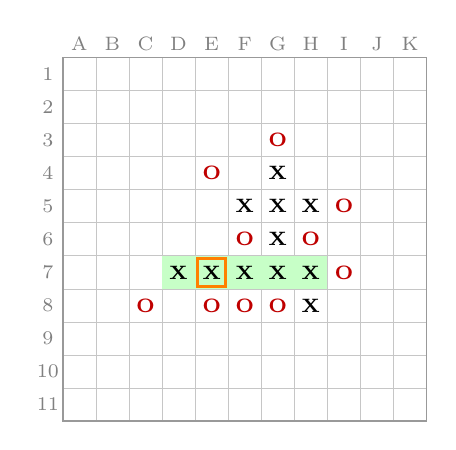
\begin{tikzpicture}[x=.42cm, y=.42cm]
\draw[gray!45, line width=.25pt] (0,0) -- (11,0);
\draw[gray!45, line width=.25pt] (0,0) -- (0,-11);
\draw[gray!45, line width=.25pt] (0,-1) -- (11,-1);
\draw[gray!45, line width=.25pt] (1,0) -- (1,-11);
\draw[gray!45, line width=.25pt] (0,-2) -- (11,-2);
\draw[gray!45, line width=.25pt] (2,0) -- (2,-11);
\draw[gray!45, line width=.25pt] (0,-3) -- (11,-3);
\draw[gray!45, line width=.25pt] (3,0) -- (3,-11);
\draw[gray!45, line width=.25pt] (0,-4) -- (11,-4);
\draw[gray!45, line width=.25pt] (4,0) -- (4,-11);
\draw[gray!45, line width=.25pt] (0,-5) -- (11,-5);
\draw[gray!45, line width=.25pt] (5,0) -- (5,-11);
\draw[gray!45, line width=.25pt] (0,-6) -- (11,-6);
\draw[gray!45, line width=.25pt] (6,0) -- (6,-11);
\draw[gray!45, line width=.25pt] (0,-7) -- (11,-7);
\draw[gray!45, line width=.25pt] (7,0) -- (7,-11);
\draw[gray!45, line width=.25pt] (0,-8) -- (11,-8);
\draw[gray!45, line width=.25pt] (8,0) -- (8,-11);
\draw[gray!45, line width=.25pt] (0,-9) -- (11,-9);
\draw[gray!45, line width=.25pt] (9,0) -- (9,-11);
\draw[gray!45, line width=.25pt] (0,-10) -- (11,-10);
\draw[gray!45, line width=.25pt] (10,0) -- (10,-11);
\draw[gray!45, line width=.25pt] (0,-11) -- (11,-11);
\draw[gray!45, line width=.25pt] (11,0) -- (11,-11);
\draw[gray!80, line width=.5pt] (0,0) rectangle (11,-11);
\node[font=\scriptsize, text=gray] at (0.5,.42) {A};
\node[font=\scriptsize, text=gray] at (1.5,.42) {B};
\node[font=\scriptsize, text=gray] at (2.5,.42) {C};
\node[font=\scriptsize, text=gray] at (3.5,.42) {D};
\node[font=\scriptsize, text=gray] at (4.5,.42) {E};
\node[font=\scriptsize, text=gray] at (5.5,.42) {F};
\node[font=\scriptsize, text=gray] at (6.5,.42) {G};
\node[font=\scriptsize, text=gray] at (7.5,.42) {H};
\node[font=\scriptsize, text=gray] at (8.5,.42) {I};
\node[font=\scriptsize, text=gray] at (9.5,.42) {J};
\node[font=\scriptsize, text=gray] at (10.5,.42) {K};
\node[font=\scriptsize, text=gray] at (-.45,-0.5) {1};
\node[font=\scriptsize, text=gray] at (-.45,-1.5) {2};
\node[font=\scriptsize, text=gray] at (-.45,-2.5) {3};
\node[font=\scriptsize, text=gray] at (-.45,-3.5) {4};
\node[font=\scriptsize, text=gray] at (-.45,-4.5) {5};
\node[font=\scriptsize, text=gray] at (-.45,-5.5) {6};
\node[font=\scriptsize, text=gray] at (-.45,-6.5) {7};
\node[font=\scriptsize, text=gray] at (-.45,-7.5) {8};
\node[font=\scriptsize, text=gray] at (-.45,-8.5) {9};
\node[font=\scriptsize, text=gray] at (-.45,-9.5) {10};
\node[font=\scriptsize, text=gray] at (-.45,-10.5) {11};
\node[text=red!75!black, font=\bfseries\scriptsize] at (6.5,-2.5) {O};
\node[text=red!75!black, font=\bfseries\scriptsize] at (4.5,-3.5) {O};
\node[text=black, font=\bfseries\scriptsize] at (6.5,-3.5) {X};
\node[text=black, font=\bfseries\scriptsize] at (5.5,-4.5) {X};
\node[text=black, font=\bfseries\scriptsize] at (6.5,-4.5) {X};
\node[text=black, font=\bfseries\scriptsize] at (7.5,-4.5) {X};
\node[text=red!75!black, font=\bfseries\scriptsize] at (8.5,-4.5) {O};
\node[text=red!75!black, font=\bfseries\scriptsize] at (5.5,-5.5) {O};
\node[text=black, font=\bfseries\scriptsize] at (6.5,-5.5) {X};
\node[text=red!75!black, font=\bfseries\scriptsize] at (7.5,-5.5) {O};
\fill[green!22] (3,-6) rectangle ++(1,-1);
\node[text=black, font=\bfseries\scriptsize] at (3.5,-6.5) {X};
\fill[green!22] (4,-6) rectangle ++(1,-1);
\node[text=black, font=\bfseries\scriptsize] at (4.5,-6.5) {X};
\draw[orange, line width=1pt] (4.08,-6.08) rectangle ++(.84,-.84);
\fill[green!22] (5,-6) rectangle ++(1,-1);
\node[text=black, font=\bfseries\scriptsize] at (5.5,-6.5) {X};
\fill[green!22] (6,-6) rectangle ++(1,-1);
\node[text=black, font=\bfseries\scriptsize] at (6.5,-6.5) {X};
\fill[green!22] (7,-6) rectangle ++(1,-1);
\node[text=black, font=\bfseries\scriptsize] at (7.5,-6.5) {X};
\node[text=red!75!black, font=\bfseries\scriptsize] at (8.5,-6.5) {O};
\node[text=red!75!black, font=\bfseries\scriptsize] at (2.5,-7.5) {O};
\node[text=red!75!black, font=\bfseries\scriptsize] at (4.5,-7.5) {O};
\node[text=red!75!black, font=\bfseries\scriptsize] at (5.5,-7.5) {O};
\node[text=red!75!black, font=\bfseries\scriptsize] at (6.5,-7.5) {O};
\node[text=black, font=\bfseries\scriptsize] at (7.5,-7.5) {X};
\end{tikzpicture}
\end{center}
\paragraph{Cơ chế kết thúc} Trước nước áp chót, bên thắng có đúng một ô thắng ngay (E7); đối thủ không chặn, nên nước E7 hoàn thành dãy.
\paragraph{Nhận xét} L8 cầm O thua nhanh trong 21 nước. Ở nước 20, X có bốn quân D7, F7, G7, H7; E7 là ô thắng duy nhất. O đi C8, X đi E7 và hoàn thành hàng ngang D7–H7. Đây là lỗi bỏ chặn duy nhất điển hình: không có đe doạ thứ hai nào buộc O phải bỏ E7. Ván này thuộc lớp lỗi mà Bảng~\ref{tab:tn-chien-thuat} đếm: L8 bỏ 1/82 lần chặn trong bộ dữ liệu L8–L3.
\paragraph{Diễn biến} {\footnotesize 1.H5 2.F8 3.G7 4.G8 5.H8 6.F6 7.H7 8.H6 9.F7 10.I7 11.G6 12.E8 13.F5 14.E4 15.G5 16.I5 17.G4 18.G3 19.D7 20.C8 21.E7\par}

\subsection{L3–L8 · ván 23}
Khai cuộc gồm 2 nước: D4 → E4. X: \texttt{L3-AlphaBeta}, O: \texttt{L8-AlphaZero}. Kết quả: O thắng sau 56 nước.
\begin{center}\small
\begin{tabular}{@{}rccll@{}}
\toprule
Ply & Màu & Nước & Nhận xét & Ô liên quan \\
\midrule
26 & O & G4 & Chặn bắt buộc & G4 \\
35 & X & H10 & Chặn bắt buộc & H10 \\
40 & O & K2 & Chặn bắt buộc & K2 \\
42 & O & A3 & Chặn bắt buộc & A3 \\
44 & O & I3 & Chặn bắt buộc & I3 \\
46 & O & C9 & Chặn bắt buộc & C9 \\
\bottomrule
\end{tabular}
\end{center}
\paragraph{Thế cờ trước nước quyết định (sau nước 45)}
\begin{center}
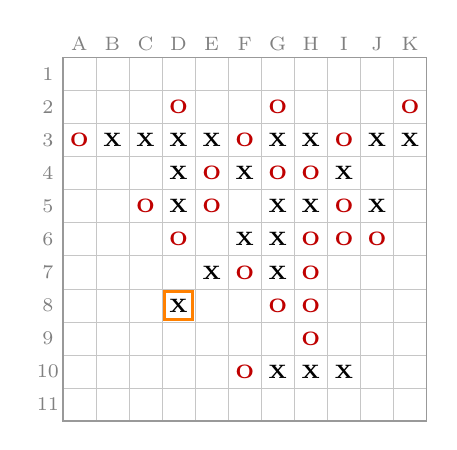
\begin{tikzpicture}[x=.42cm, y=.42cm]
\draw[gray!45, line width=.25pt] (0,0) -- (11,0);
\draw[gray!45, line width=.25pt] (0,0) -- (0,-11);
\draw[gray!45, line width=.25pt] (0,-1) -- (11,-1);
\draw[gray!45, line width=.25pt] (1,0) -- (1,-11);
\draw[gray!45, line width=.25pt] (0,-2) -- (11,-2);
\draw[gray!45, line width=.25pt] (2,0) -- (2,-11);
\draw[gray!45, line width=.25pt] (0,-3) -- (11,-3);
\draw[gray!45, line width=.25pt] (3,0) -- (3,-11);
\draw[gray!45, line width=.25pt] (0,-4) -- (11,-4);
\draw[gray!45, line width=.25pt] (4,0) -- (4,-11);
\draw[gray!45, line width=.25pt] (0,-5) -- (11,-5);
\draw[gray!45, line width=.25pt] (5,0) -- (5,-11);
\draw[gray!45, line width=.25pt] (0,-6) -- (11,-6);
\draw[gray!45, line width=.25pt] (6,0) -- (6,-11);
\draw[gray!45, line width=.25pt] (0,-7) -- (11,-7);
\draw[gray!45, line width=.25pt] (7,0) -- (7,-11);
\draw[gray!45, line width=.25pt] (0,-8) -- (11,-8);
\draw[gray!45, line width=.25pt] (8,0) -- (8,-11);
\draw[gray!45, line width=.25pt] (0,-9) -- (11,-9);
\draw[gray!45, line width=.25pt] (9,0) -- (9,-11);
\draw[gray!45, line width=.25pt] (0,-10) -- (11,-10);
\draw[gray!45, line width=.25pt] (10,0) -- (10,-11);
\draw[gray!45, line width=.25pt] (0,-11) -- (11,-11);
\draw[gray!45, line width=.25pt] (11,0) -- (11,-11);
\draw[gray!80, line width=.5pt] (0,0) rectangle (11,-11);
\node[font=\scriptsize, text=gray] at (0.5,.42) {A};
\node[font=\scriptsize, text=gray] at (1.5,.42) {B};
\node[font=\scriptsize, text=gray] at (2.5,.42) {C};
\node[font=\scriptsize, text=gray] at (3.5,.42) {D};
\node[font=\scriptsize, text=gray] at (4.5,.42) {E};
\node[font=\scriptsize, text=gray] at (5.5,.42) {F};
\node[font=\scriptsize, text=gray] at (6.5,.42) {G};
\node[font=\scriptsize, text=gray] at (7.5,.42) {H};
\node[font=\scriptsize, text=gray] at (8.5,.42) {I};
\node[font=\scriptsize, text=gray] at (9.5,.42) {J};
\node[font=\scriptsize, text=gray] at (10.5,.42) {K};
\node[font=\scriptsize, text=gray] at (-.45,-0.5) {1};
\node[font=\scriptsize, text=gray] at (-.45,-1.5) {2};
\node[font=\scriptsize, text=gray] at (-.45,-2.5) {3};
\node[font=\scriptsize, text=gray] at (-.45,-3.5) {4};
\node[font=\scriptsize, text=gray] at (-.45,-4.5) {5};
\node[font=\scriptsize, text=gray] at (-.45,-5.5) {6};
\node[font=\scriptsize, text=gray] at (-.45,-6.5) {7};
\node[font=\scriptsize, text=gray] at (-.45,-7.5) {8};
\node[font=\scriptsize, text=gray] at (-.45,-8.5) {9};
\node[font=\scriptsize, text=gray] at (-.45,-9.5) {10};
\node[font=\scriptsize, text=gray] at (-.45,-10.5) {11};
\node[text=red!75!black, font=\bfseries\scriptsize] at (3.5,-1.5) {O};
\node[text=red!75!black, font=\bfseries\scriptsize] at (6.5,-1.5) {O};
\node[text=red!75!black, font=\bfseries\scriptsize] at (10.5,-1.5) {O};
\node[text=red!75!black, font=\bfseries\scriptsize] at (0.5,-2.5) {O};
\node[text=black, font=\bfseries\scriptsize] at (1.5,-2.5) {X};
\node[text=black, font=\bfseries\scriptsize] at (2.5,-2.5) {X};
\node[text=black, font=\bfseries\scriptsize] at (3.5,-2.5) {X};
\node[text=black, font=\bfseries\scriptsize] at (4.5,-2.5) {X};
\node[text=red!75!black, font=\bfseries\scriptsize] at (5.5,-2.5) {O};
\node[text=black, font=\bfseries\scriptsize] at (6.5,-2.5) {X};
\node[text=black, font=\bfseries\scriptsize] at (7.5,-2.5) {X};
\node[text=red!75!black, font=\bfseries\scriptsize] at (8.5,-2.5) {O};
\node[text=black, font=\bfseries\scriptsize] at (9.5,-2.5) {X};
\node[text=black, font=\bfseries\scriptsize] at (10.5,-2.5) {X};
\node[text=black, font=\bfseries\scriptsize] at (3.5,-3.5) {X};
\node[text=red!75!black, font=\bfseries\scriptsize] at (4.5,-3.5) {O};
\node[text=black, font=\bfseries\scriptsize] at (5.5,-3.5) {X};
\node[text=red!75!black, font=\bfseries\scriptsize] at (6.5,-3.5) {O};
\node[text=red!75!black, font=\bfseries\scriptsize] at (7.5,-3.5) {O};
\node[text=black, font=\bfseries\scriptsize] at (8.5,-3.5) {X};
\node[text=red!75!black, font=\bfseries\scriptsize] at (2.5,-4.5) {O};
\node[text=black, font=\bfseries\scriptsize] at (3.5,-4.5) {X};
\node[text=red!75!black, font=\bfseries\scriptsize] at (4.5,-4.5) {O};
\node[text=black, font=\bfseries\scriptsize] at (6.5,-4.5) {X};
\node[text=black, font=\bfseries\scriptsize] at (7.5,-4.5) {X};
\node[text=red!75!black, font=\bfseries\scriptsize] at (8.5,-4.5) {O};
\node[text=black, font=\bfseries\scriptsize] at (9.5,-4.5) {X};
\node[text=red!75!black, font=\bfseries\scriptsize] at (3.5,-5.5) {O};
\node[text=black, font=\bfseries\scriptsize] at (5.5,-5.5) {X};
\node[text=black, font=\bfseries\scriptsize] at (6.5,-5.5) {X};
\node[text=red!75!black, font=\bfseries\scriptsize] at (7.5,-5.5) {O};
\node[text=red!75!black, font=\bfseries\scriptsize] at (8.5,-5.5) {O};
\node[text=red!75!black, font=\bfseries\scriptsize] at (9.5,-5.5) {O};
\node[text=black, font=\bfseries\scriptsize] at (4.5,-6.5) {X};
\node[text=red!75!black, font=\bfseries\scriptsize] at (5.5,-6.5) {O};
\node[text=black, font=\bfseries\scriptsize] at (6.5,-6.5) {X};
\node[text=red!75!black, font=\bfseries\scriptsize] at (7.5,-6.5) {O};
\node[text=black, font=\bfseries\scriptsize] at (3.5,-7.5) {X};
\draw[orange, line width=1pt] (3.08,-7.08) rectangle ++(.84,-.84);
\node[text=red!75!black, font=\bfseries\scriptsize] at (6.5,-7.5) {O};
\node[text=red!75!black, font=\bfseries\scriptsize] at (7.5,-7.5) {O};
\node[text=red!75!black, font=\bfseries\scriptsize] at (7.5,-8.5) {O};
\node[text=red!75!black, font=\bfseries\scriptsize] at (5.5,-9.5) {O};
\node[text=black, font=\bfseries\scriptsize] at (6.5,-9.5) {X};
\node[text=black, font=\bfseries\scriptsize] at (7.5,-9.5) {X};
\node[text=black, font=\bfseries\scriptsize] at (8.5,-9.5) {X};
\end{tikzpicture}
\end{center}
\paragraph{Thế kết thúc}
\begin{center}
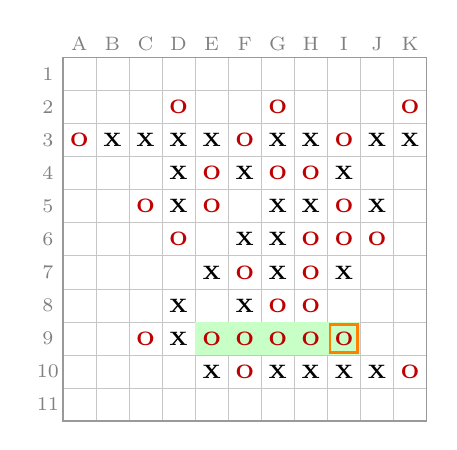
\begin{tikzpicture}[x=.42cm, y=.42cm]
\draw[gray!45, line width=.25pt] (0,0) -- (11,0);
\draw[gray!45, line width=.25pt] (0,0) -- (0,-11);
\draw[gray!45, line width=.25pt] (0,-1) -- (11,-1);
\draw[gray!45, line width=.25pt] (1,0) -- (1,-11);
\draw[gray!45, line width=.25pt] (0,-2) -- (11,-2);
\draw[gray!45, line width=.25pt] (2,0) -- (2,-11);
\draw[gray!45, line width=.25pt] (0,-3) -- (11,-3);
\draw[gray!45, line width=.25pt] (3,0) -- (3,-11);
\draw[gray!45, line width=.25pt] (0,-4) -- (11,-4);
\draw[gray!45, line width=.25pt] (4,0) -- (4,-11);
\draw[gray!45, line width=.25pt] (0,-5) -- (11,-5);
\draw[gray!45, line width=.25pt] (5,0) -- (5,-11);
\draw[gray!45, line width=.25pt] (0,-6) -- (11,-6);
\draw[gray!45, line width=.25pt] (6,0) -- (6,-11);
\draw[gray!45, line width=.25pt] (0,-7) -- (11,-7);
\draw[gray!45, line width=.25pt] (7,0) -- (7,-11);
\draw[gray!45, line width=.25pt] (0,-8) -- (11,-8);
\draw[gray!45, line width=.25pt] (8,0) -- (8,-11);
\draw[gray!45, line width=.25pt] (0,-9) -- (11,-9);
\draw[gray!45, line width=.25pt] (9,0) -- (9,-11);
\draw[gray!45, line width=.25pt] (0,-10) -- (11,-10);
\draw[gray!45, line width=.25pt] (10,0) -- (10,-11);
\draw[gray!45, line width=.25pt] (0,-11) -- (11,-11);
\draw[gray!45, line width=.25pt] (11,0) -- (11,-11);
\draw[gray!80, line width=.5pt] (0,0) rectangle (11,-11);
\node[font=\scriptsize, text=gray] at (0.5,.42) {A};
\node[font=\scriptsize, text=gray] at (1.5,.42) {B};
\node[font=\scriptsize, text=gray] at (2.5,.42) {C};
\node[font=\scriptsize, text=gray] at (3.5,.42) {D};
\node[font=\scriptsize, text=gray] at (4.5,.42) {E};
\node[font=\scriptsize, text=gray] at (5.5,.42) {F};
\node[font=\scriptsize, text=gray] at (6.5,.42) {G};
\node[font=\scriptsize, text=gray] at (7.5,.42) {H};
\node[font=\scriptsize, text=gray] at (8.5,.42) {I};
\node[font=\scriptsize, text=gray] at (9.5,.42) {J};
\node[font=\scriptsize, text=gray] at (10.5,.42) {K};
\node[font=\scriptsize, text=gray] at (-.45,-0.5) {1};
\node[font=\scriptsize, text=gray] at (-.45,-1.5) {2};
\node[font=\scriptsize, text=gray] at (-.45,-2.5) {3};
\node[font=\scriptsize, text=gray] at (-.45,-3.5) {4};
\node[font=\scriptsize, text=gray] at (-.45,-4.5) {5};
\node[font=\scriptsize, text=gray] at (-.45,-5.5) {6};
\node[font=\scriptsize, text=gray] at (-.45,-6.5) {7};
\node[font=\scriptsize, text=gray] at (-.45,-7.5) {8};
\node[font=\scriptsize, text=gray] at (-.45,-8.5) {9};
\node[font=\scriptsize, text=gray] at (-.45,-9.5) {10};
\node[font=\scriptsize, text=gray] at (-.45,-10.5) {11};
\node[text=red!75!black, font=\bfseries\scriptsize] at (3.5,-1.5) {O};
\node[text=red!75!black, font=\bfseries\scriptsize] at (6.5,-1.5) {O};
\node[text=red!75!black, font=\bfseries\scriptsize] at (10.5,-1.5) {O};
\node[text=red!75!black, font=\bfseries\scriptsize] at (0.5,-2.5) {O};
\node[text=black, font=\bfseries\scriptsize] at (1.5,-2.5) {X};
\node[text=black, font=\bfseries\scriptsize] at (2.5,-2.5) {X};
\node[text=black, font=\bfseries\scriptsize] at (3.5,-2.5) {X};
\node[text=black, font=\bfseries\scriptsize] at (4.5,-2.5) {X};
\node[text=red!75!black, font=\bfseries\scriptsize] at (5.5,-2.5) {O};
\node[text=black, font=\bfseries\scriptsize] at (6.5,-2.5) {X};
\node[text=black, font=\bfseries\scriptsize] at (7.5,-2.5) {X};
\node[text=red!75!black, font=\bfseries\scriptsize] at (8.5,-2.5) {O};
\node[text=black, font=\bfseries\scriptsize] at (9.5,-2.5) {X};
\node[text=black, font=\bfseries\scriptsize] at (10.5,-2.5) {X};
\node[text=black, font=\bfseries\scriptsize] at (3.5,-3.5) {X};
\node[text=red!75!black, font=\bfseries\scriptsize] at (4.5,-3.5) {O};
\node[text=black, font=\bfseries\scriptsize] at (5.5,-3.5) {X};
\node[text=red!75!black, font=\bfseries\scriptsize] at (6.5,-3.5) {O};
\node[text=red!75!black, font=\bfseries\scriptsize] at (7.5,-3.5) {O};
\node[text=black, font=\bfseries\scriptsize] at (8.5,-3.5) {X};
\node[text=red!75!black, font=\bfseries\scriptsize] at (2.5,-4.5) {O};
\node[text=black, font=\bfseries\scriptsize] at (3.5,-4.5) {X};
\node[text=red!75!black, font=\bfseries\scriptsize] at (4.5,-4.5) {O};
\node[text=black, font=\bfseries\scriptsize] at (6.5,-4.5) {X};
\node[text=black, font=\bfseries\scriptsize] at (7.5,-4.5) {X};
\node[text=red!75!black, font=\bfseries\scriptsize] at (8.5,-4.5) {O};
\node[text=black, font=\bfseries\scriptsize] at (9.5,-4.5) {X};
\node[text=red!75!black, font=\bfseries\scriptsize] at (3.5,-5.5) {O};
\node[text=black, font=\bfseries\scriptsize] at (5.5,-5.5) {X};
\node[text=black, font=\bfseries\scriptsize] at (6.5,-5.5) {X};
\node[text=red!75!black, font=\bfseries\scriptsize] at (7.5,-5.5) {O};
\node[text=red!75!black, font=\bfseries\scriptsize] at (8.5,-5.5) {O};
\node[text=red!75!black, font=\bfseries\scriptsize] at (9.5,-5.5) {O};
\node[text=black, font=\bfseries\scriptsize] at (4.5,-6.5) {X};
\node[text=red!75!black, font=\bfseries\scriptsize] at (5.5,-6.5) {O};
\node[text=black, font=\bfseries\scriptsize] at (6.5,-6.5) {X};
\node[text=red!75!black, font=\bfseries\scriptsize] at (7.5,-6.5) {O};
\node[text=black, font=\bfseries\scriptsize] at (8.5,-6.5) {X};
\node[text=black, font=\bfseries\scriptsize] at (3.5,-7.5) {X};
\node[text=black, font=\bfseries\scriptsize] at (5.5,-7.5) {X};
\node[text=red!75!black, font=\bfseries\scriptsize] at (6.5,-7.5) {O};
\node[text=red!75!black, font=\bfseries\scriptsize] at (7.5,-7.5) {O};
\node[text=red!75!black, font=\bfseries\scriptsize] at (2.5,-8.5) {O};
\node[text=black, font=\bfseries\scriptsize] at (3.5,-8.5) {X};
\fill[green!22] (4,-8) rectangle ++(1,-1);
\node[text=red!75!black, font=\bfseries\scriptsize] at (4.5,-8.5) {O};
\fill[green!22] (5,-8) rectangle ++(1,-1);
\node[text=red!75!black, font=\bfseries\scriptsize] at (5.5,-8.5) {O};
\fill[green!22] (6,-8) rectangle ++(1,-1);
\node[text=red!75!black, font=\bfseries\scriptsize] at (6.5,-8.5) {O};
\fill[green!22] (7,-8) rectangle ++(1,-1);
\node[text=red!75!black, font=\bfseries\scriptsize] at (7.5,-8.5) {O};
\fill[green!22] (8,-8) rectangle ++(1,-1);
\node[text=red!75!black, font=\bfseries\scriptsize] at (8.5,-8.5) {O};
\draw[orange, line width=1pt] (8.08,-8.08) rectangle ++(.84,-.84);
\node[text=black, font=\bfseries\scriptsize] at (4.5,-9.5) {X};
\node[text=red!75!black, font=\bfseries\scriptsize] at (5.5,-9.5) {O};
\node[text=black, font=\bfseries\scriptsize] at (6.5,-9.5) {X};
\node[text=black, font=\bfseries\scriptsize] at (7.5,-9.5) {X};
\node[text=black, font=\bfseries\scriptsize] at (8.5,-9.5) {X};
\node[text=black, font=\bfseries\scriptsize] at (9.5,-9.5) {X};
\node[text=red!75!black, font=\bfseries\scriptsize] at (10.5,-9.5) {O};
\end{tikzpicture}
\end{center}
\paragraph{Cơ chế kết thúc} Trước nước áp chót, bên thắng đã có 2 ô thắng ngay (D9, I9); đối thủ chỉ chặn được một ô, nên nước I9 hoàn thành dãy năm quân.
\paragraph{Nhận xét} L8 cầm O thắng sau 56 nước, ván dài nhất trong nhóm O thắng. O kiên trì xây dựng hàng ngang E9–I9; trước nước 55, hai đầu D9 và I9 đều là ô thắng. X chặn D9, O đi I9. Ván này cho thấy L8 có thể chơi phòng thủ dài rồi phản công, không chỉ thắng nhanh bằng đe doạ sớm.
\paragraph{Diễn biến} {\footnotesize 1.D4 2.E4 3.E3 4.C5 5.C3 6.E5 7.D3 8.F3 9.D5 10.D6 11.F4 12.D2 13.E7 14.F7 15.G5 16.H6 17.F6 18.H4 19.H5 20.I5 21.G7 22.J6 23.G3 24.I6 25.G6 26.G4 27.I4 28.G8 29.J5 30.H9 31.I10 32.H8 33.H3 34.H7 35.H10 36.G2 37.G10 38.F10 39.J3 40.K2 41.B3 42.A3 43.K3 44.I3 45.D8 46.C9 47.J10 48.K10 49.F8 50.G9 51.I7 52.F9 53.E10 54.E9 55.D9 56.I9\par}

\subsection{L8–L3 · ván 03}
Khai cuộc gồm 2 nước: D4 → E4. X: \texttt{L8-AlphaZero}, O: \texttt{L3-AlphaBeta}. Kết quả: hoà sau 121 nước.
\begin{center}\small
\begin{tabular}{@{}rccll@{}}
\toprule
Ply & Màu & Nước & Nhận xét & Ô liên quan \\
\midrule
13 & X & E2 & Chặn bắt buộc & E2 \\
22 & O & B11 & Chặn bắt buộc & B11 \\
24 & O & A4 & Chặn bắt buộc & A4 \\
27 & X & A2 & Chặn bắt buộc & A2 \\
30 & O & E11 & Chặn bắt buộc & E11 \\
40 & O & A9 & Chặn bắt buộc & A9 \\
\bottomrule
\end{tabular}
\end{center}
\paragraph{Thế cờ trước nước quyết định (sau nước 39)}
\begin{center}
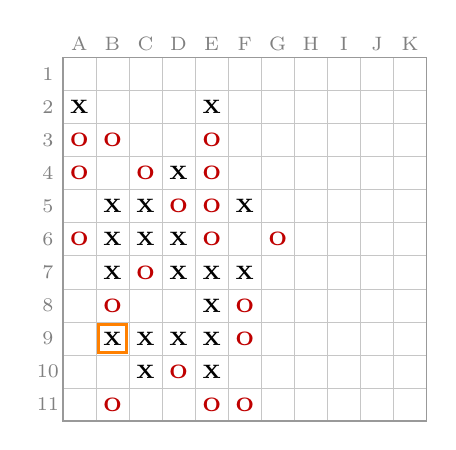
\begin{tikzpicture}[x=.42cm, y=.42cm]
\draw[gray!45, line width=.25pt] (0,0) -- (11,0);
\draw[gray!45, line width=.25pt] (0,0) -- (0,-11);
\draw[gray!45, line width=.25pt] (0,-1) -- (11,-1);
\draw[gray!45, line width=.25pt] (1,0) -- (1,-11);
\draw[gray!45, line width=.25pt] (0,-2) -- (11,-2);
\draw[gray!45, line width=.25pt] (2,0) -- (2,-11);
\draw[gray!45, line width=.25pt] (0,-3) -- (11,-3);
\draw[gray!45, line width=.25pt] (3,0) -- (3,-11);
\draw[gray!45, line width=.25pt] (0,-4) -- (11,-4);
\draw[gray!45, line width=.25pt] (4,0) -- (4,-11);
\draw[gray!45, line width=.25pt] (0,-5) -- (11,-5);
\draw[gray!45, line width=.25pt] (5,0) -- (5,-11);
\draw[gray!45, line width=.25pt] (0,-6) -- (11,-6);
\draw[gray!45, line width=.25pt] (6,0) -- (6,-11);
\draw[gray!45, line width=.25pt] (0,-7) -- (11,-7);
\draw[gray!45, line width=.25pt] (7,0) -- (7,-11);
\draw[gray!45, line width=.25pt] (0,-8) -- (11,-8);
\draw[gray!45, line width=.25pt] (8,0) -- (8,-11);
\draw[gray!45, line width=.25pt] (0,-9) -- (11,-9);
\draw[gray!45, line width=.25pt] (9,0) -- (9,-11);
\draw[gray!45, line width=.25pt] (0,-10) -- (11,-10);
\draw[gray!45, line width=.25pt] (10,0) -- (10,-11);
\draw[gray!45, line width=.25pt] (0,-11) -- (11,-11);
\draw[gray!45, line width=.25pt] (11,0) -- (11,-11);
\draw[gray!80, line width=.5pt] (0,0) rectangle (11,-11);
\node[font=\scriptsize, text=gray] at (0.5,.42) {A};
\node[font=\scriptsize, text=gray] at (1.5,.42) {B};
\node[font=\scriptsize, text=gray] at (2.5,.42) {C};
\node[font=\scriptsize, text=gray] at (3.5,.42) {D};
\node[font=\scriptsize, text=gray] at (4.5,.42) {E};
\node[font=\scriptsize, text=gray] at (5.5,.42) {F};
\node[font=\scriptsize, text=gray] at (6.5,.42) {G};
\node[font=\scriptsize, text=gray] at (7.5,.42) {H};
\node[font=\scriptsize, text=gray] at (8.5,.42) {I};
\node[font=\scriptsize, text=gray] at (9.5,.42) {J};
\node[font=\scriptsize, text=gray] at (10.5,.42) {K};
\node[font=\scriptsize, text=gray] at (-.45,-0.5) {1};
\node[font=\scriptsize, text=gray] at (-.45,-1.5) {2};
\node[font=\scriptsize, text=gray] at (-.45,-2.5) {3};
\node[font=\scriptsize, text=gray] at (-.45,-3.5) {4};
\node[font=\scriptsize, text=gray] at (-.45,-4.5) {5};
\node[font=\scriptsize, text=gray] at (-.45,-5.5) {6};
\node[font=\scriptsize, text=gray] at (-.45,-6.5) {7};
\node[font=\scriptsize, text=gray] at (-.45,-7.5) {8};
\node[font=\scriptsize, text=gray] at (-.45,-8.5) {9};
\node[font=\scriptsize, text=gray] at (-.45,-9.5) {10};
\node[font=\scriptsize, text=gray] at (-.45,-10.5) {11};
\node[text=black, font=\bfseries\scriptsize] at (0.5,-1.5) {X};
\node[text=black, font=\bfseries\scriptsize] at (4.5,-1.5) {X};
\node[text=red!75!black, font=\bfseries\scriptsize] at (0.5,-2.5) {O};
\node[text=red!75!black, font=\bfseries\scriptsize] at (1.5,-2.5) {O};
\node[text=red!75!black, font=\bfseries\scriptsize] at (4.5,-2.5) {O};
\node[text=red!75!black, font=\bfseries\scriptsize] at (0.5,-3.5) {O};
\node[text=red!75!black, font=\bfseries\scriptsize] at (2.5,-3.5) {O};
\node[text=black, font=\bfseries\scriptsize] at (3.5,-3.5) {X};
\node[text=red!75!black, font=\bfseries\scriptsize] at (4.5,-3.5) {O};
\node[text=black, font=\bfseries\scriptsize] at (1.5,-4.5) {X};
\node[text=black, font=\bfseries\scriptsize] at (2.5,-4.5) {X};
\node[text=red!75!black, font=\bfseries\scriptsize] at (3.5,-4.5) {O};
\node[text=red!75!black, font=\bfseries\scriptsize] at (4.5,-4.5) {O};
\node[text=black, font=\bfseries\scriptsize] at (5.5,-4.5) {X};
\node[text=red!75!black, font=\bfseries\scriptsize] at (0.5,-5.5) {O};
\node[text=black, font=\bfseries\scriptsize] at (1.5,-5.5) {X};
\node[text=black, font=\bfseries\scriptsize] at (2.5,-5.5) {X};
\node[text=black, font=\bfseries\scriptsize] at (3.5,-5.5) {X};
\node[text=red!75!black, font=\bfseries\scriptsize] at (4.5,-5.5) {O};
\node[text=red!75!black, font=\bfseries\scriptsize] at (6.5,-5.5) {O};
\node[text=black, font=\bfseries\scriptsize] at (1.5,-6.5) {X};
\node[text=red!75!black, font=\bfseries\scriptsize] at (2.5,-6.5) {O};
\node[text=black, font=\bfseries\scriptsize] at (3.5,-6.5) {X};
\node[text=black, font=\bfseries\scriptsize] at (4.5,-6.5) {X};
\node[text=black, font=\bfseries\scriptsize] at (5.5,-6.5) {X};
\node[text=red!75!black, font=\bfseries\scriptsize] at (1.5,-7.5) {O};
\node[text=black, font=\bfseries\scriptsize] at (4.5,-7.5) {X};
\node[text=red!75!black, font=\bfseries\scriptsize] at (5.5,-7.5) {O};
\node[text=black, font=\bfseries\scriptsize] at (1.5,-8.5) {X};
\draw[orange, line width=1pt] (1.08,-8.08) rectangle ++(.84,-.84);
\node[text=black, font=\bfseries\scriptsize] at (2.5,-8.5) {X};
\node[text=black, font=\bfseries\scriptsize] at (3.5,-8.5) {X};
\node[text=black, font=\bfseries\scriptsize] at (4.5,-8.5) {X};
\node[text=red!75!black, font=\bfseries\scriptsize] at (5.5,-8.5) {O};
\node[text=black, font=\bfseries\scriptsize] at (2.5,-9.5) {X};
\node[text=red!75!black, font=\bfseries\scriptsize] at (3.5,-9.5) {O};
\node[text=black, font=\bfseries\scriptsize] at (4.5,-9.5) {X};
\node[text=red!75!black, font=\bfseries\scriptsize] at (1.5,-10.5) {O};
\node[text=red!75!black, font=\bfseries\scriptsize] at (4.5,-10.5) {O};
\node[text=red!75!black, font=\bfseries\scriptsize] at (5.5,-10.5) {O};
\end{tikzpicture}
\end{center}
\paragraph{Thế kết thúc}
\begin{center}
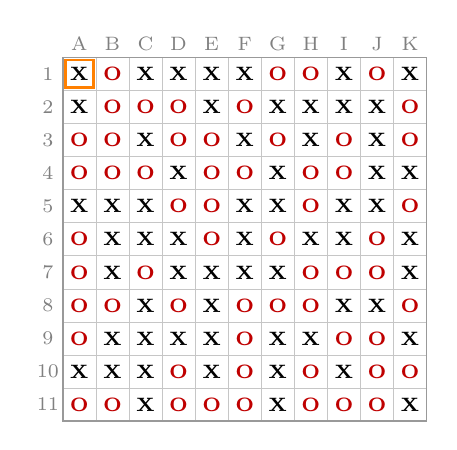
\begin{tikzpicture}[x=.42cm, y=.42cm]
\draw[gray!45, line width=.25pt] (0,0) -- (11,0);
\draw[gray!45, line width=.25pt] (0,0) -- (0,-11);
\draw[gray!45, line width=.25pt] (0,-1) -- (11,-1);
\draw[gray!45, line width=.25pt] (1,0) -- (1,-11);
\draw[gray!45, line width=.25pt] (0,-2) -- (11,-2);
\draw[gray!45, line width=.25pt] (2,0) -- (2,-11);
\draw[gray!45, line width=.25pt] (0,-3) -- (11,-3);
\draw[gray!45, line width=.25pt] (3,0) -- (3,-11);
\draw[gray!45, line width=.25pt] (0,-4) -- (11,-4);
\draw[gray!45, line width=.25pt] (4,0) -- (4,-11);
\draw[gray!45, line width=.25pt] (0,-5) -- (11,-5);
\draw[gray!45, line width=.25pt] (5,0) -- (5,-11);
\draw[gray!45, line width=.25pt] (0,-6) -- (11,-6);
\draw[gray!45, line width=.25pt] (6,0) -- (6,-11);
\draw[gray!45, line width=.25pt] (0,-7) -- (11,-7);
\draw[gray!45, line width=.25pt] (7,0) -- (7,-11);
\draw[gray!45, line width=.25pt] (0,-8) -- (11,-8);
\draw[gray!45, line width=.25pt] (8,0) -- (8,-11);
\draw[gray!45, line width=.25pt] (0,-9) -- (11,-9);
\draw[gray!45, line width=.25pt] (9,0) -- (9,-11);
\draw[gray!45, line width=.25pt] (0,-10) -- (11,-10);
\draw[gray!45, line width=.25pt] (10,0) -- (10,-11);
\draw[gray!45, line width=.25pt] (0,-11) -- (11,-11);
\draw[gray!45, line width=.25pt] (11,0) -- (11,-11);
\draw[gray!80, line width=.5pt] (0,0) rectangle (11,-11);
\node[font=\scriptsize, text=gray] at (0.5,.42) {A};
\node[font=\scriptsize, text=gray] at (1.5,.42) {B};
\node[font=\scriptsize, text=gray] at (2.5,.42) {C};
\node[font=\scriptsize, text=gray] at (3.5,.42) {D};
\node[font=\scriptsize, text=gray] at (4.5,.42) {E};
\node[font=\scriptsize, text=gray] at (5.5,.42) {F};
\node[font=\scriptsize, text=gray] at (6.5,.42) {G};
\node[font=\scriptsize, text=gray] at (7.5,.42) {H};
\node[font=\scriptsize, text=gray] at (8.5,.42) {I};
\node[font=\scriptsize, text=gray] at (9.5,.42) {J};
\node[font=\scriptsize, text=gray] at (10.5,.42) {K};
\node[font=\scriptsize, text=gray] at (-.45,-0.5) {1};
\node[font=\scriptsize, text=gray] at (-.45,-1.5) {2};
\node[font=\scriptsize, text=gray] at (-.45,-2.5) {3};
\node[font=\scriptsize, text=gray] at (-.45,-3.5) {4};
\node[font=\scriptsize, text=gray] at (-.45,-4.5) {5};
\node[font=\scriptsize, text=gray] at (-.45,-5.5) {6};
\node[font=\scriptsize, text=gray] at (-.45,-6.5) {7};
\node[font=\scriptsize, text=gray] at (-.45,-7.5) {8};
\node[font=\scriptsize, text=gray] at (-.45,-8.5) {9};
\node[font=\scriptsize, text=gray] at (-.45,-9.5) {10};
\node[font=\scriptsize, text=gray] at (-.45,-10.5) {11};
\node[text=black, font=\bfseries\scriptsize] at (0.5,-0.5) {X};
\draw[orange, line width=1pt] (0.08,-0.08) rectangle ++(.84,-.84);
\node[text=red!75!black, font=\bfseries\scriptsize] at (1.5,-0.5) {O};
\node[text=black, font=\bfseries\scriptsize] at (2.5,-0.5) {X};
\node[text=black, font=\bfseries\scriptsize] at (3.5,-0.5) {X};
\node[text=black, font=\bfseries\scriptsize] at (4.5,-0.5) {X};
\node[text=black, font=\bfseries\scriptsize] at (5.5,-0.5) {X};
\node[text=red!75!black, font=\bfseries\scriptsize] at (6.5,-0.5) {O};
\node[text=red!75!black, font=\bfseries\scriptsize] at (7.5,-0.5) {O};
\node[text=black, font=\bfseries\scriptsize] at (8.5,-0.5) {X};
\node[text=red!75!black, font=\bfseries\scriptsize] at (9.5,-0.5) {O};
\node[text=black, font=\bfseries\scriptsize] at (10.5,-0.5) {X};
\node[text=black, font=\bfseries\scriptsize] at (0.5,-1.5) {X};
\node[text=red!75!black, font=\bfseries\scriptsize] at (1.5,-1.5) {O};
\node[text=red!75!black, font=\bfseries\scriptsize] at (2.5,-1.5) {O};
\node[text=red!75!black, font=\bfseries\scriptsize] at (3.5,-1.5) {O};
\node[text=black, font=\bfseries\scriptsize] at (4.5,-1.5) {X};
\node[text=red!75!black, font=\bfseries\scriptsize] at (5.5,-1.5) {O};
\node[text=black, font=\bfseries\scriptsize] at (6.5,-1.5) {X};
\node[text=black, font=\bfseries\scriptsize] at (7.5,-1.5) {X};
\node[text=black, font=\bfseries\scriptsize] at (8.5,-1.5) {X};
\node[text=black, font=\bfseries\scriptsize] at (9.5,-1.5) {X};
\node[text=red!75!black, font=\bfseries\scriptsize] at (10.5,-1.5) {O};
\node[text=red!75!black, font=\bfseries\scriptsize] at (0.5,-2.5) {O};
\node[text=red!75!black, font=\bfseries\scriptsize] at (1.5,-2.5) {O};
\node[text=black, font=\bfseries\scriptsize] at (2.5,-2.5) {X};
\node[text=red!75!black, font=\bfseries\scriptsize] at (3.5,-2.5) {O};
\node[text=red!75!black, font=\bfseries\scriptsize] at (4.5,-2.5) {O};
\node[text=black, font=\bfseries\scriptsize] at (5.5,-2.5) {X};
\node[text=red!75!black, font=\bfseries\scriptsize] at (6.5,-2.5) {O};
\node[text=black, font=\bfseries\scriptsize] at (7.5,-2.5) {X};
\node[text=red!75!black, font=\bfseries\scriptsize] at (8.5,-2.5) {O};
\node[text=black, font=\bfseries\scriptsize] at (9.5,-2.5) {X};
\node[text=red!75!black, font=\bfseries\scriptsize] at (10.5,-2.5) {O};
\node[text=red!75!black, font=\bfseries\scriptsize] at (0.5,-3.5) {O};
\node[text=red!75!black, font=\bfseries\scriptsize] at (1.5,-3.5) {O};
\node[text=red!75!black, font=\bfseries\scriptsize] at (2.5,-3.5) {O};
\node[text=black, font=\bfseries\scriptsize] at (3.5,-3.5) {X};
\node[text=red!75!black, font=\bfseries\scriptsize] at (4.5,-3.5) {O};
\node[text=red!75!black, font=\bfseries\scriptsize] at (5.5,-3.5) {O};
\node[text=black, font=\bfseries\scriptsize] at (6.5,-3.5) {X};
\node[text=red!75!black, font=\bfseries\scriptsize] at (7.5,-3.5) {O};
\node[text=red!75!black, font=\bfseries\scriptsize] at (8.5,-3.5) {O};
\node[text=black, font=\bfseries\scriptsize] at (9.5,-3.5) {X};
\node[text=black, font=\bfseries\scriptsize] at (10.5,-3.5) {X};
\node[text=black, font=\bfseries\scriptsize] at (0.5,-4.5) {X};
\node[text=black, font=\bfseries\scriptsize] at (1.5,-4.5) {X};
\node[text=black, font=\bfseries\scriptsize] at (2.5,-4.5) {X};
\node[text=red!75!black, font=\bfseries\scriptsize] at (3.5,-4.5) {O};
\node[text=red!75!black, font=\bfseries\scriptsize] at (4.5,-4.5) {O};
\node[text=black, font=\bfseries\scriptsize] at (5.5,-4.5) {X};
\node[text=black, font=\bfseries\scriptsize] at (6.5,-4.5) {X};
\node[text=red!75!black, font=\bfseries\scriptsize] at (7.5,-4.5) {O};
\node[text=black, font=\bfseries\scriptsize] at (8.5,-4.5) {X};
\node[text=black, font=\bfseries\scriptsize] at (9.5,-4.5) {X};
\node[text=red!75!black, font=\bfseries\scriptsize] at (10.5,-4.5) {O};
\node[text=red!75!black, font=\bfseries\scriptsize] at (0.5,-5.5) {O};
\node[text=black, font=\bfseries\scriptsize] at (1.5,-5.5) {X};
\node[text=black, font=\bfseries\scriptsize] at (2.5,-5.5) {X};
\node[text=black, font=\bfseries\scriptsize] at (3.5,-5.5) {X};
\node[text=red!75!black, font=\bfseries\scriptsize] at (4.5,-5.5) {O};
\node[text=black, font=\bfseries\scriptsize] at (5.5,-5.5) {X};
\node[text=red!75!black, font=\bfseries\scriptsize] at (6.5,-5.5) {O};
\node[text=black, font=\bfseries\scriptsize] at (7.5,-5.5) {X};
\node[text=black, font=\bfseries\scriptsize] at (8.5,-5.5) {X};
\node[text=red!75!black, font=\bfseries\scriptsize] at (9.5,-5.5) {O};
\node[text=black, font=\bfseries\scriptsize] at (10.5,-5.5) {X};
\node[text=red!75!black, font=\bfseries\scriptsize] at (0.5,-6.5) {O};
\node[text=black, font=\bfseries\scriptsize] at (1.5,-6.5) {X};
\node[text=red!75!black, font=\bfseries\scriptsize] at (2.5,-6.5) {O};
\node[text=black, font=\bfseries\scriptsize] at (3.5,-6.5) {X};
\node[text=black, font=\bfseries\scriptsize] at (4.5,-6.5) {X};
\node[text=black, font=\bfseries\scriptsize] at (5.5,-6.5) {X};
\node[text=black, font=\bfseries\scriptsize] at (6.5,-6.5) {X};
\node[text=red!75!black, font=\bfseries\scriptsize] at (7.5,-6.5) {O};
\node[text=red!75!black, font=\bfseries\scriptsize] at (8.5,-6.5) {O};
\node[text=red!75!black, font=\bfseries\scriptsize] at (9.5,-6.5) {O};
\node[text=black, font=\bfseries\scriptsize] at (10.5,-6.5) {X};
\node[text=red!75!black, font=\bfseries\scriptsize] at (0.5,-7.5) {O};
\node[text=red!75!black, font=\bfseries\scriptsize] at (1.5,-7.5) {O};
\node[text=black, font=\bfseries\scriptsize] at (2.5,-7.5) {X};
\node[text=red!75!black, font=\bfseries\scriptsize] at (3.5,-7.5) {O};
\node[text=black, font=\bfseries\scriptsize] at (4.5,-7.5) {X};
\node[text=red!75!black, font=\bfseries\scriptsize] at (5.5,-7.5) {O};
\node[text=red!75!black, font=\bfseries\scriptsize] at (6.5,-7.5) {O};
\node[text=red!75!black, font=\bfseries\scriptsize] at (7.5,-7.5) {O};
\node[text=black, font=\bfseries\scriptsize] at (8.5,-7.5) {X};
\node[text=black, font=\bfseries\scriptsize] at (9.5,-7.5) {X};
\node[text=red!75!black, font=\bfseries\scriptsize] at (10.5,-7.5) {O};
\node[text=red!75!black, font=\bfseries\scriptsize] at (0.5,-8.5) {O};
\node[text=black, font=\bfseries\scriptsize] at (1.5,-8.5) {X};
\node[text=black, font=\bfseries\scriptsize] at (2.5,-8.5) {X};
\node[text=black, font=\bfseries\scriptsize] at (3.5,-8.5) {X};
\node[text=black, font=\bfseries\scriptsize] at (4.5,-8.5) {X};
\node[text=red!75!black, font=\bfseries\scriptsize] at (5.5,-8.5) {O};
\node[text=black, font=\bfseries\scriptsize] at (6.5,-8.5) {X};
\node[text=black, font=\bfseries\scriptsize] at (7.5,-8.5) {X};
\node[text=red!75!black, font=\bfseries\scriptsize] at (8.5,-8.5) {O};
\node[text=red!75!black, font=\bfseries\scriptsize] at (9.5,-8.5) {O};
\node[text=black, font=\bfseries\scriptsize] at (10.5,-8.5) {X};
\node[text=black, font=\bfseries\scriptsize] at (0.5,-9.5) {X};
\node[text=black, font=\bfseries\scriptsize] at (1.5,-9.5) {X};
\node[text=black, font=\bfseries\scriptsize] at (2.5,-9.5) {X};
\node[text=red!75!black, font=\bfseries\scriptsize] at (3.5,-9.5) {O};
\node[text=black, font=\bfseries\scriptsize] at (4.5,-9.5) {X};
\node[text=red!75!black, font=\bfseries\scriptsize] at (5.5,-9.5) {O};
\node[text=black, font=\bfseries\scriptsize] at (6.5,-9.5) {X};
\node[text=red!75!black, font=\bfseries\scriptsize] at (7.5,-9.5) {O};
\node[text=black, font=\bfseries\scriptsize] at (8.5,-9.5) {X};
\node[text=red!75!black, font=\bfseries\scriptsize] at (9.5,-9.5) {O};
\node[text=red!75!black, font=\bfseries\scriptsize] at (10.5,-9.5) {O};
\node[text=red!75!black, font=\bfseries\scriptsize] at (0.5,-10.5) {O};
\node[text=red!75!black, font=\bfseries\scriptsize] at (1.5,-10.5) {O};
\node[text=black, font=\bfseries\scriptsize] at (2.5,-10.5) {X};
\node[text=red!75!black, font=\bfseries\scriptsize] at (3.5,-10.5) {O};
\node[text=red!75!black, font=\bfseries\scriptsize] at (4.5,-10.5) {O};
\node[text=red!75!black, font=\bfseries\scriptsize] at (5.5,-10.5) {O};
\node[text=black, font=\bfseries\scriptsize] at (6.5,-10.5) {X};
\node[text=red!75!black, font=\bfseries\scriptsize] at (7.5,-10.5) {O};
\node[text=red!75!black, font=\bfseries\scriptsize] at (8.5,-10.5) {O};
\node[text=red!75!black, font=\bfseries\scriptsize] at (9.5,-10.5) {O};
\node[text=black, font=\bfseries\scriptsize] at (10.5,-10.5) {X};
\end{tikzpicture}
\end{center}
\paragraph{Cơ chế kết thúc} Bàn đầy mà không bên nào có năm quân liên tiếp; kết quả là hoà.
\paragraph{Nhận xét} Ván hoà duy nhất của cặp L8–L3 khi L8 cầm X, kéo dài đủ 121 nước. Bàn đầy mà không bên nào có năm quân. Đây là bằng chứng L3 có thể phòng thủ đủ để cầm hoà trước L8 trong một số khai cuộc, dù L8 mạnh hơn về tổng thể. Ván hoà cũng cho thấy kết quả không chỉ có thắng/thua; với luật tự do, hoà là trạng thái hiếm nhưng có thật.
\paragraph{Diễn biến} {\footnotesize 1.D4 2.E4 3.D6 4.D5 5.C6 6.E6 7.C5 8.C4 9.F7 10.E3 11.E7 12.E5 13.E2 14.F8 15.D7 16.C7 17.E8 18.F9 19.D9 20.G6 21.C10 22.B11 23.B5 24.A4 25.E10 26.B3 27.A2 28.D10 29.E9 30.E11 31.B7 32.F11 33.B6 34.B8 35.F5 36.A3 37.C9 38.A6 39.B9 40.A9 41.F6 42.D8 43.F3 44.F4 45.G5 46.H4 47.G4 48.H5 49.H3 50.H11 51.G11 52.H7 53.I2 54.J1 55.G2 56.G3 57.H2 58.F2 59.I5 60.H8 61.H6 62.I4 63.H9 64.G8 65.J8 66.K2 67.J3 68.I7 69.G9 70.I9 71.I8 72.A7 73.A5 74.A11 75.J5 76.J7 77.G7 78.K3 79.A10 80.G1 81.J4 82.J6 83.C11 84.H1 85.I1 86.D2 87.E1 88.K10 89.C1 90.K8 91.D1 92.B1 93.K7 94.J10 95.K11 96.D3 97.C3 98.H10 99.I10 100.K5 101.K4 102.J11 103.K9 104.I11 105.K6 106.D11 107.G10 108.F10 109.B10 110.J9 111.C8 112.A8 113.I6 114.B4 115.J2 116.I3 117.F1 118.C2 119.K1 120.B2 121.A1\par}

\subsection{L8–L7 · ván 12}
Khai cuộc gồm 2 nước: F7 → E4. X: \texttt{L8}, O: \texttt{L7-PUCT[l5]}. Kết quả: X thắng sau 21 nước.
\begin{center}\small
\begin{tabular}{@{}rccll@{}}
\toprule
Ply & Màu & Nước & Nhận xét & Ô liên quan \\
\midrule
13 & X & E6 & Chặn bắt buộc & E6 \\
17 & X & E1 & Chặn bắt buộc & E1 \\
20 & O & J6 & Đã ở thế buộc thua & — \\
21 & X & C8 & Thắng ngay & — \\
\bottomrule
\end{tabular}
\end{center}
\paragraph{Thế cờ trước nước quyết định (sau nước 20)}
\begin{center}
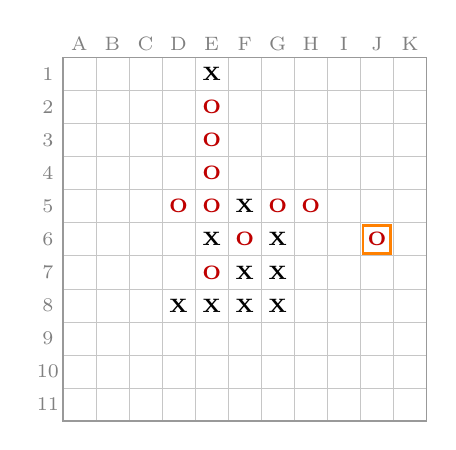
\begin{tikzpicture}[x=.42cm, y=.42cm]
\draw[gray!45, line width=.25pt] (0,0) -- (11,0);
\draw[gray!45, line width=.25pt] (0,0) -- (0,-11);
\draw[gray!45, line width=.25pt] (0,-1) -- (11,-1);
\draw[gray!45, line width=.25pt] (1,0) -- (1,-11);
\draw[gray!45, line width=.25pt] (0,-2) -- (11,-2);
\draw[gray!45, line width=.25pt] (2,0) -- (2,-11);
\draw[gray!45, line width=.25pt] (0,-3) -- (11,-3);
\draw[gray!45, line width=.25pt] (3,0) -- (3,-11);
\draw[gray!45, line width=.25pt] (0,-4) -- (11,-4);
\draw[gray!45, line width=.25pt] (4,0) -- (4,-11);
\draw[gray!45, line width=.25pt] (0,-5) -- (11,-5);
\draw[gray!45, line width=.25pt] (5,0) -- (5,-11);
\draw[gray!45, line width=.25pt] (0,-6) -- (11,-6);
\draw[gray!45, line width=.25pt] (6,0) -- (6,-11);
\draw[gray!45, line width=.25pt] (0,-7) -- (11,-7);
\draw[gray!45, line width=.25pt] (7,0) -- (7,-11);
\draw[gray!45, line width=.25pt] (0,-8) -- (11,-8);
\draw[gray!45, line width=.25pt] (8,0) -- (8,-11);
\draw[gray!45, line width=.25pt] (0,-9) -- (11,-9);
\draw[gray!45, line width=.25pt] (9,0) -- (9,-11);
\draw[gray!45, line width=.25pt] (0,-10) -- (11,-10);
\draw[gray!45, line width=.25pt] (10,0) -- (10,-11);
\draw[gray!45, line width=.25pt] (0,-11) -- (11,-11);
\draw[gray!45, line width=.25pt] (11,0) -- (11,-11);
\draw[gray!80, line width=.5pt] (0,0) rectangle (11,-11);
\node[font=\scriptsize, text=gray] at (0.5,.42) {A};
\node[font=\scriptsize, text=gray] at (1.5,.42) {B};
\node[font=\scriptsize, text=gray] at (2.5,.42) {C};
\node[font=\scriptsize, text=gray] at (3.5,.42) {D};
\node[font=\scriptsize, text=gray] at (4.5,.42) {E};
\node[font=\scriptsize, text=gray] at (5.5,.42) {F};
\node[font=\scriptsize, text=gray] at (6.5,.42) {G};
\node[font=\scriptsize, text=gray] at (7.5,.42) {H};
\node[font=\scriptsize, text=gray] at (8.5,.42) {I};
\node[font=\scriptsize, text=gray] at (9.5,.42) {J};
\node[font=\scriptsize, text=gray] at (10.5,.42) {K};
\node[font=\scriptsize, text=gray] at (-.45,-0.5) {1};
\node[font=\scriptsize, text=gray] at (-.45,-1.5) {2};
\node[font=\scriptsize, text=gray] at (-.45,-2.5) {3};
\node[font=\scriptsize, text=gray] at (-.45,-3.5) {4};
\node[font=\scriptsize, text=gray] at (-.45,-4.5) {5};
\node[font=\scriptsize, text=gray] at (-.45,-5.5) {6};
\node[font=\scriptsize, text=gray] at (-.45,-6.5) {7};
\node[font=\scriptsize, text=gray] at (-.45,-7.5) {8};
\node[font=\scriptsize, text=gray] at (-.45,-8.5) {9};
\node[font=\scriptsize, text=gray] at (-.45,-9.5) {10};
\node[font=\scriptsize, text=gray] at (-.45,-10.5) {11};
\node[text=black, font=\bfseries\scriptsize] at (4.5,-0.5) {X};
\node[text=red!75!black, font=\bfseries\scriptsize] at (4.5,-1.5) {O};
\node[text=red!75!black, font=\bfseries\scriptsize] at (4.5,-2.5) {O};
\node[text=red!75!black, font=\bfseries\scriptsize] at (4.5,-3.5) {O};
\node[text=red!75!black, font=\bfseries\scriptsize] at (3.5,-4.5) {O};
\node[text=red!75!black, font=\bfseries\scriptsize] at (4.5,-4.5) {O};
\node[text=black, font=\bfseries\scriptsize] at (5.5,-4.5) {X};
\node[text=red!75!black, font=\bfseries\scriptsize] at (6.5,-4.5) {O};
\node[text=red!75!black, font=\bfseries\scriptsize] at (7.5,-4.5) {O};
\node[text=black, font=\bfseries\scriptsize] at (4.5,-5.5) {X};
\node[text=red!75!black, font=\bfseries\scriptsize] at (5.5,-5.5) {O};
\node[text=black, font=\bfseries\scriptsize] at (6.5,-5.5) {X};
\node[text=red!75!black, font=\bfseries\scriptsize] at (9.5,-5.5) {O};
\draw[orange, line width=1pt] (9.08,-5.08) rectangle ++(.84,-.84);
\node[text=red!75!black, font=\bfseries\scriptsize] at (4.5,-6.5) {O};
\node[text=black, font=\bfseries\scriptsize] at (5.5,-6.5) {X};
\node[text=black, font=\bfseries\scriptsize] at (6.5,-6.5) {X};
\node[text=black, font=\bfseries\scriptsize] at (3.5,-7.5) {X};
\node[text=black, font=\bfseries\scriptsize] at (4.5,-7.5) {X};
\node[text=black, font=\bfseries\scriptsize] at (5.5,-7.5) {X};
\node[text=black, font=\bfseries\scriptsize] at (6.5,-7.5) {X};
\end{tikzpicture}
\end{center}
\paragraph{Thế kết thúc}
\begin{center}
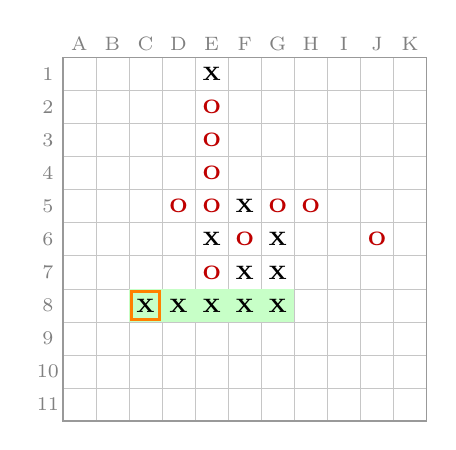
\begin{tikzpicture}[x=.42cm, y=.42cm]
\draw[gray!45, line width=.25pt] (0,0) -- (11,0);
\draw[gray!45, line width=.25pt] (0,0) -- (0,-11);
\draw[gray!45, line width=.25pt] (0,-1) -- (11,-1);
\draw[gray!45, line width=.25pt] (1,0) -- (1,-11);
\draw[gray!45, line width=.25pt] (0,-2) -- (11,-2);
\draw[gray!45, line width=.25pt] (2,0) -- (2,-11);
\draw[gray!45, line width=.25pt] (0,-3) -- (11,-3);
\draw[gray!45, line width=.25pt] (3,0) -- (3,-11);
\draw[gray!45, line width=.25pt] (0,-4) -- (11,-4);
\draw[gray!45, line width=.25pt] (4,0) -- (4,-11);
\draw[gray!45, line width=.25pt] (0,-5) -- (11,-5);
\draw[gray!45, line width=.25pt] (5,0) -- (5,-11);
\draw[gray!45, line width=.25pt] (0,-6) -- (11,-6);
\draw[gray!45, line width=.25pt] (6,0) -- (6,-11);
\draw[gray!45, line width=.25pt] (0,-7) -- (11,-7);
\draw[gray!45, line width=.25pt] (7,0) -- (7,-11);
\draw[gray!45, line width=.25pt] (0,-8) -- (11,-8);
\draw[gray!45, line width=.25pt] (8,0) -- (8,-11);
\draw[gray!45, line width=.25pt] (0,-9) -- (11,-9);
\draw[gray!45, line width=.25pt] (9,0) -- (9,-11);
\draw[gray!45, line width=.25pt] (0,-10) -- (11,-10);
\draw[gray!45, line width=.25pt] (10,0) -- (10,-11);
\draw[gray!45, line width=.25pt] (0,-11) -- (11,-11);
\draw[gray!45, line width=.25pt] (11,0) -- (11,-11);
\draw[gray!80, line width=.5pt] (0,0) rectangle (11,-11);
\node[font=\scriptsize, text=gray] at (0.5,.42) {A};
\node[font=\scriptsize, text=gray] at (1.5,.42) {B};
\node[font=\scriptsize, text=gray] at (2.5,.42) {C};
\node[font=\scriptsize, text=gray] at (3.5,.42) {D};
\node[font=\scriptsize, text=gray] at (4.5,.42) {E};
\node[font=\scriptsize, text=gray] at (5.5,.42) {F};
\node[font=\scriptsize, text=gray] at (6.5,.42) {G};
\node[font=\scriptsize, text=gray] at (7.5,.42) {H};
\node[font=\scriptsize, text=gray] at (8.5,.42) {I};
\node[font=\scriptsize, text=gray] at (9.5,.42) {J};
\node[font=\scriptsize, text=gray] at (10.5,.42) {K};
\node[font=\scriptsize, text=gray] at (-.45,-0.5) {1};
\node[font=\scriptsize, text=gray] at (-.45,-1.5) {2};
\node[font=\scriptsize, text=gray] at (-.45,-2.5) {3};
\node[font=\scriptsize, text=gray] at (-.45,-3.5) {4};
\node[font=\scriptsize, text=gray] at (-.45,-4.5) {5};
\node[font=\scriptsize, text=gray] at (-.45,-5.5) {6};
\node[font=\scriptsize, text=gray] at (-.45,-6.5) {7};
\node[font=\scriptsize, text=gray] at (-.45,-7.5) {8};
\node[font=\scriptsize, text=gray] at (-.45,-8.5) {9};
\node[font=\scriptsize, text=gray] at (-.45,-9.5) {10};
\node[font=\scriptsize, text=gray] at (-.45,-10.5) {11};
\node[text=black, font=\bfseries\scriptsize] at (4.5,-0.5) {X};
\node[text=red!75!black, font=\bfseries\scriptsize] at (4.5,-1.5) {O};
\node[text=red!75!black, font=\bfseries\scriptsize] at (4.5,-2.5) {O};
\node[text=red!75!black, font=\bfseries\scriptsize] at (4.5,-3.5) {O};
\node[text=red!75!black, font=\bfseries\scriptsize] at (3.5,-4.5) {O};
\node[text=red!75!black, font=\bfseries\scriptsize] at (4.5,-4.5) {O};
\node[text=black, font=\bfseries\scriptsize] at (5.5,-4.5) {X};
\node[text=red!75!black, font=\bfseries\scriptsize] at (6.5,-4.5) {O};
\node[text=red!75!black, font=\bfseries\scriptsize] at (7.5,-4.5) {O};
\node[text=black, font=\bfseries\scriptsize] at (4.5,-5.5) {X};
\node[text=red!75!black, font=\bfseries\scriptsize] at (5.5,-5.5) {O};
\node[text=black, font=\bfseries\scriptsize] at (6.5,-5.5) {X};
\node[text=red!75!black, font=\bfseries\scriptsize] at (9.5,-5.5) {O};
\node[text=red!75!black, font=\bfseries\scriptsize] at (4.5,-6.5) {O};
\node[text=black, font=\bfseries\scriptsize] at (5.5,-6.5) {X};
\node[text=black, font=\bfseries\scriptsize] at (6.5,-6.5) {X};
\fill[green!22] (2,-7) rectangle ++(1,-1);
\node[text=black, font=\bfseries\scriptsize] at (2.5,-7.5) {X};
\draw[orange, line width=1pt] (2.08,-7.08) rectangle ++(.84,-.84);
\fill[green!22] (3,-7) rectangle ++(1,-1);
\node[text=black, font=\bfseries\scriptsize] at (3.5,-7.5) {X};
\fill[green!22] (4,-7) rectangle ++(1,-1);
\node[text=black, font=\bfseries\scriptsize] at (4.5,-7.5) {X};
\fill[green!22] (5,-7) rectangle ++(1,-1);
\node[text=black, font=\bfseries\scriptsize] at (5.5,-7.5) {X};
\fill[green!22] (6,-7) rectangle ++(1,-1);
\node[text=black, font=\bfseries\scriptsize] at (6.5,-7.5) {X};
\end{tikzpicture}
\end{center}
\paragraph{Cơ chế kết thúc} Trước nước áp chót, bên thắng đã có 2 ô thắng ngay (C8, H8); đối thủ chỉ chặn được một ô, nên nước C8 hoàn thành dãy năm quân.
\paragraph{Nhận xét} L8 cầm X thắng L7 trong 21 nước bằng hàng ngang C8–G8. Trước nước cuối, X có bốn quân D8–G8; hai đầu C8 và H8 là ô thắng. O đi J6, X đi C8. Đòn kép hai đầu lại xuất hiện, lần này ở hàng ngang. Ván minh hoạ L8 chuyển từ trung tâm sang cánh phải để tạo đe doạ ngang.
\paragraph{Diễn biến} {\footnotesize 1.F7 2.E4 3.G7 4.E7 5.G6 6.G5 7.E8 8.H5 9.G8 10.E5 11.F5 12.E3 13.E6 14.D5 15.F8 16.E2 17.E1 18.F6 19.D8 20.J6 21.C8\par}

\subsection{L8–L7 · ván 08}
Khai cuộc gồm 3 nước: G7 → F5 → F8. X: \texttt{L8}, O: \texttt{L7-PUCT[l5]}. Kết quả: O thắng sau 24 nước.
\begin{center}\small
\begin{tabular}{@{}rccll@{}}
\toprule
Ply & Màu & Nước & Nhận xét & Ô liên quan \\
\midrule
12 & O & K9 & Chặn bắt buộc & K9 \\
16 & O & D10 & Chặn bắt buộc & D10 \\
18 & O & H7 & Chặn bắt buộc & H7 \\
20 & O & D7 & Chặn bắt buộc & D7 \\
23 & X & E8 & Đã ở thế buộc thua & — \\
24 & O & K8 & Thắng ngay & — \\
\bottomrule
\end{tabular}
\end{center}
\paragraph{Thế cờ trước nước quyết định (sau nước 23)}
\begin{center}
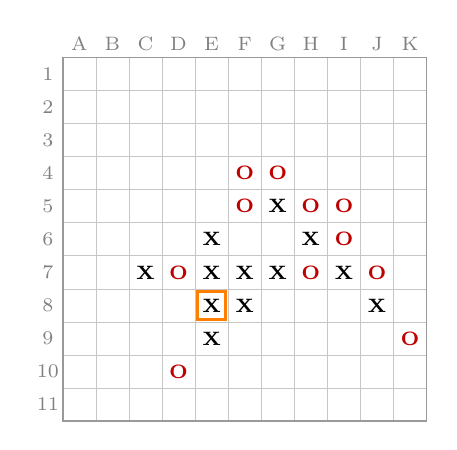
\begin{tikzpicture}[x=.42cm, y=.42cm]
\draw[gray!45, line width=.25pt] (0,0) -- (11,0);
\draw[gray!45, line width=.25pt] (0,0) -- (0,-11);
\draw[gray!45, line width=.25pt] (0,-1) -- (11,-1);
\draw[gray!45, line width=.25pt] (1,0) -- (1,-11);
\draw[gray!45, line width=.25pt] (0,-2) -- (11,-2);
\draw[gray!45, line width=.25pt] (2,0) -- (2,-11);
\draw[gray!45, line width=.25pt] (0,-3) -- (11,-3);
\draw[gray!45, line width=.25pt] (3,0) -- (3,-11);
\draw[gray!45, line width=.25pt] (0,-4) -- (11,-4);
\draw[gray!45, line width=.25pt] (4,0) -- (4,-11);
\draw[gray!45, line width=.25pt] (0,-5) -- (11,-5);
\draw[gray!45, line width=.25pt] (5,0) -- (5,-11);
\draw[gray!45, line width=.25pt] (0,-6) -- (11,-6);
\draw[gray!45, line width=.25pt] (6,0) -- (6,-11);
\draw[gray!45, line width=.25pt] (0,-7) -- (11,-7);
\draw[gray!45, line width=.25pt] (7,0) -- (7,-11);
\draw[gray!45, line width=.25pt] (0,-8) -- (11,-8);
\draw[gray!45, line width=.25pt] (8,0) -- (8,-11);
\draw[gray!45, line width=.25pt] (0,-9) -- (11,-9);
\draw[gray!45, line width=.25pt] (9,0) -- (9,-11);
\draw[gray!45, line width=.25pt] (0,-10) -- (11,-10);
\draw[gray!45, line width=.25pt] (10,0) -- (10,-11);
\draw[gray!45, line width=.25pt] (0,-11) -- (11,-11);
\draw[gray!45, line width=.25pt] (11,0) -- (11,-11);
\draw[gray!80, line width=.5pt] (0,0) rectangle (11,-11);
\node[font=\scriptsize, text=gray] at (0.5,.42) {A};
\node[font=\scriptsize, text=gray] at (1.5,.42) {B};
\node[font=\scriptsize, text=gray] at (2.5,.42) {C};
\node[font=\scriptsize, text=gray] at (3.5,.42) {D};
\node[font=\scriptsize, text=gray] at (4.5,.42) {E};
\node[font=\scriptsize, text=gray] at (5.5,.42) {F};
\node[font=\scriptsize, text=gray] at (6.5,.42) {G};
\node[font=\scriptsize, text=gray] at (7.5,.42) {H};
\node[font=\scriptsize, text=gray] at (8.5,.42) {I};
\node[font=\scriptsize, text=gray] at (9.5,.42) {J};
\node[font=\scriptsize, text=gray] at (10.5,.42) {K};
\node[font=\scriptsize, text=gray] at (-.45,-0.5) {1};
\node[font=\scriptsize, text=gray] at (-.45,-1.5) {2};
\node[font=\scriptsize, text=gray] at (-.45,-2.5) {3};
\node[font=\scriptsize, text=gray] at (-.45,-3.5) {4};
\node[font=\scriptsize, text=gray] at (-.45,-4.5) {5};
\node[font=\scriptsize, text=gray] at (-.45,-5.5) {6};
\node[font=\scriptsize, text=gray] at (-.45,-6.5) {7};
\node[font=\scriptsize, text=gray] at (-.45,-7.5) {8};
\node[font=\scriptsize, text=gray] at (-.45,-8.5) {9};
\node[font=\scriptsize, text=gray] at (-.45,-9.5) {10};
\node[font=\scriptsize, text=gray] at (-.45,-10.5) {11};
\node[text=red!75!black, font=\bfseries\scriptsize] at (5.5,-3.5) {O};
\node[text=red!75!black, font=\bfseries\scriptsize] at (6.5,-3.5) {O};
\node[text=red!75!black, font=\bfseries\scriptsize] at (5.5,-4.5) {O};
\node[text=black, font=\bfseries\scriptsize] at (6.5,-4.5) {X};
\node[text=red!75!black, font=\bfseries\scriptsize] at (7.5,-4.5) {O};
\node[text=red!75!black, font=\bfseries\scriptsize] at (8.5,-4.5) {O};
\node[text=black, font=\bfseries\scriptsize] at (4.5,-5.5) {X};
\node[text=black, font=\bfseries\scriptsize] at (7.5,-5.5) {X};
\node[text=red!75!black, font=\bfseries\scriptsize] at (8.5,-5.5) {O};
\node[text=black, font=\bfseries\scriptsize] at (2.5,-6.5) {X};
\node[text=red!75!black, font=\bfseries\scriptsize] at (3.5,-6.5) {O};
\node[text=black, font=\bfseries\scriptsize] at (4.5,-6.5) {X};
\node[text=black, font=\bfseries\scriptsize] at (5.5,-6.5) {X};
\node[text=black, font=\bfseries\scriptsize] at (6.5,-6.5) {X};
\node[text=red!75!black, font=\bfseries\scriptsize] at (7.5,-6.5) {O};
\node[text=black, font=\bfseries\scriptsize] at (8.5,-6.5) {X};
\node[text=red!75!black, font=\bfseries\scriptsize] at (9.5,-6.5) {O};
\node[text=black, font=\bfseries\scriptsize] at (4.5,-7.5) {X};
\draw[orange, line width=1pt] (4.08,-7.08) rectangle ++(.84,-.84);
\node[text=black, font=\bfseries\scriptsize] at (5.5,-7.5) {X};
\node[text=black, font=\bfseries\scriptsize] at (9.5,-7.5) {X};
\node[text=black, font=\bfseries\scriptsize] at (4.5,-8.5) {X};
\node[text=red!75!black, font=\bfseries\scriptsize] at (10.5,-8.5) {O};
\node[text=red!75!black, font=\bfseries\scriptsize] at (3.5,-9.5) {O};
\end{tikzpicture}
\end{center}
\paragraph{Thế kết thúc}
\begin{center}
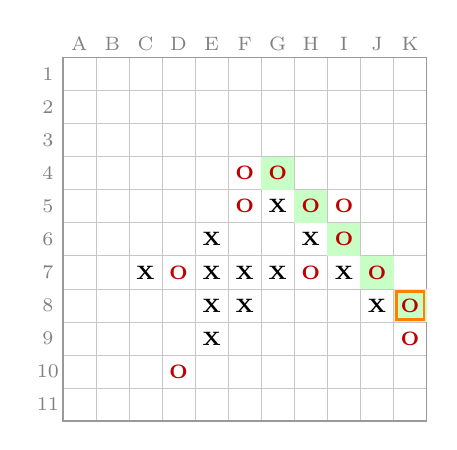
\begin{tikzpicture}[x=.42cm, y=.42cm]
\draw[gray!45, line width=.25pt] (0,0) -- (11,0);
\draw[gray!45, line width=.25pt] (0,0) -- (0,-11);
\draw[gray!45, line width=.25pt] (0,-1) -- (11,-1);
\draw[gray!45, line width=.25pt] (1,0) -- (1,-11);
\draw[gray!45, line width=.25pt] (0,-2) -- (11,-2);
\draw[gray!45, line width=.25pt] (2,0) -- (2,-11);
\draw[gray!45, line width=.25pt] (0,-3) -- (11,-3);
\draw[gray!45, line width=.25pt] (3,0) -- (3,-11);
\draw[gray!45, line width=.25pt] (0,-4) -- (11,-4);
\draw[gray!45, line width=.25pt] (4,0) -- (4,-11);
\draw[gray!45, line width=.25pt] (0,-5) -- (11,-5);
\draw[gray!45, line width=.25pt] (5,0) -- (5,-11);
\draw[gray!45, line width=.25pt] (0,-6) -- (11,-6);
\draw[gray!45, line width=.25pt] (6,0) -- (6,-11);
\draw[gray!45, line width=.25pt] (0,-7) -- (11,-7);
\draw[gray!45, line width=.25pt] (7,0) -- (7,-11);
\draw[gray!45, line width=.25pt] (0,-8) -- (11,-8);
\draw[gray!45, line width=.25pt] (8,0) -- (8,-11);
\draw[gray!45, line width=.25pt] (0,-9) -- (11,-9);
\draw[gray!45, line width=.25pt] (9,0) -- (9,-11);
\draw[gray!45, line width=.25pt] (0,-10) -- (11,-10);
\draw[gray!45, line width=.25pt] (10,0) -- (10,-11);
\draw[gray!45, line width=.25pt] (0,-11) -- (11,-11);
\draw[gray!45, line width=.25pt] (11,0) -- (11,-11);
\draw[gray!80, line width=.5pt] (0,0) rectangle (11,-11);
\node[font=\scriptsize, text=gray] at (0.5,.42) {A};
\node[font=\scriptsize, text=gray] at (1.5,.42) {B};
\node[font=\scriptsize, text=gray] at (2.5,.42) {C};
\node[font=\scriptsize, text=gray] at (3.5,.42) {D};
\node[font=\scriptsize, text=gray] at (4.5,.42) {E};
\node[font=\scriptsize, text=gray] at (5.5,.42) {F};
\node[font=\scriptsize, text=gray] at (6.5,.42) {G};
\node[font=\scriptsize, text=gray] at (7.5,.42) {H};
\node[font=\scriptsize, text=gray] at (8.5,.42) {I};
\node[font=\scriptsize, text=gray] at (9.5,.42) {J};
\node[font=\scriptsize, text=gray] at (10.5,.42) {K};
\node[font=\scriptsize, text=gray] at (-.45,-0.5) {1};
\node[font=\scriptsize, text=gray] at (-.45,-1.5) {2};
\node[font=\scriptsize, text=gray] at (-.45,-2.5) {3};
\node[font=\scriptsize, text=gray] at (-.45,-3.5) {4};
\node[font=\scriptsize, text=gray] at (-.45,-4.5) {5};
\node[font=\scriptsize, text=gray] at (-.45,-5.5) {6};
\node[font=\scriptsize, text=gray] at (-.45,-6.5) {7};
\node[font=\scriptsize, text=gray] at (-.45,-7.5) {8};
\node[font=\scriptsize, text=gray] at (-.45,-8.5) {9};
\node[font=\scriptsize, text=gray] at (-.45,-9.5) {10};
\node[font=\scriptsize, text=gray] at (-.45,-10.5) {11};
\node[text=red!75!black, font=\bfseries\scriptsize] at (5.5,-3.5) {O};
\fill[green!22] (6,-3) rectangle ++(1,-1);
\node[text=red!75!black, font=\bfseries\scriptsize] at (6.5,-3.5) {O};
\node[text=red!75!black, font=\bfseries\scriptsize] at (5.5,-4.5) {O};
\node[text=black, font=\bfseries\scriptsize] at (6.5,-4.5) {X};
\fill[green!22] (7,-4) rectangle ++(1,-1);
\node[text=red!75!black, font=\bfseries\scriptsize] at (7.5,-4.5) {O};
\node[text=red!75!black, font=\bfseries\scriptsize] at (8.5,-4.5) {O};
\node[text=black, font=\bfseries\scriptsize] at (4.5,-5.5) {X};
\node[text=black, font=\bfseries\scriptsize] at (7.5,-5.5) {X};
\fill[green!22] (8,-5) rectangle ++(1,-1);
\node[text=red!75!black, font=\bfseries\scriptsize] at (8.5,-5.5) {O};
\node[text=black, font=\bfseries\scriptsize] at (2.5,-6.5) {X};
\node[text=red!75!black, font=\bfseries\scriptsize] at (3.5,-6.5) {O};
\node[text=black, font=\bfseries\scriptsize] at (4.5,-6.5) {X};
\node[text=black, font=\bfseries\scriptsize] at (5.5,-6.5) {X};
\node[text=black, font=\bfseries\scriptsize] at (6.5,-6.5) {X};
\node[text=red!75!black, font=\bfseries\scriptsize] at (7.5,-6.5) {O};
\node[text=black, font=\bfseries\scriptsize] at (8.5,-6.5) {X};
\fill[green!22] (9,-6) rectangle ++(1,-1);
\node[text=red!75!black, font=\bfseries\scriptsize] at (9.5,-6.5) {O};
\node[text=black, font=\bfseries\scriptsize] at (4.5,-7.5) {X};
\node[text=black, font=\bfseries\scriptsize] at (5.5,-7.5) {X};
\node[text=black, font=\bfseries\scriptsize] at (9.5,-7.5) {X};
\fill[green!22] (10,-7) rectangle ++(1,-1);
\node[text=red!75!black, font=\bfseries\scriptsize] at (10.5,-7.5) {O};
\draw[orange, line width=1pt] (10.08,-7.08) rectangle ++(.84,-.84);
\node[text=black, font=\bfseries\scriptsize] at (4.5,-8.5) {X};
\node[text=red!75!black, font=\bfseries\scriptsize] at (10.5,-8.5) {O};
\node[text=red!75!black, font=\bfseries\scriptsize] at (3.5,-9.5) {O};
\end{tikzpicture}
\end{center}
\paragraph{Cơ chế kết thúc} Trước nước áp chót, bên thắng đã có 2 ô thắng ngay (F3, K8); đối thủ chỉ chặn được một ô, nên nước K8 hoàn thành dãy năm quân.
\paragraph{Nhận xét} L8 cầm X thua L7 trong 24 nước. O thắng bằng đường chéo G4–K8; trước nước 23, hai đầu F3 và K8 là ô thắng. X đi E8, O đi K8. Không có lỗi bỏ chặn đơn; X bị buộc phải chọn giữa hai đầu. Đây là ví dụ thua vì đối thủ tạo đòn kép, không phải vì bỏ sót một nước cứu.
\paragraph{Diễn biến} {\footnotesize 1.G7 2.F5 3.F8 4.H5 5.H6 6.I5 7.G5 8.G4 9.I7 10.F4 11.J8 12.K9 13.F7 14.J7 15.E9 16.D10 17.E7 18.H7 19.C7 20.D7 21.E6 22.I6 23.E8 24.K8\par}

\subsection{L7–L8 · ván 19}
Khai cuộc gồm 4 nước: H6 → E6 → F6 → D6. X: \texttt{L7-PUCT[l5]}, O: \texttt{L8}. Kết quả: X thắng sau 21 nước.
\begin{center}\small
\begin{tabular}{@{}rccll@{}}
\toprule
Ply & Màu & Nước & Nhận xét & Ô liên quan \\
\midrule
16 & O & K7 & Chặn bắt buộc & K7 \\
18 & O & I6 & Chặn bắt buộc & I6 \\
20 & O & G7 & Đã ở thế buộc thua & — \\
21 & X & G2 & Thắng ngay & — \\
\bottomrule
\end{tabular}
\end{center}
\paragraph{Thế cờ trước nước quyết định (sau nước 20)}
\begin{center}
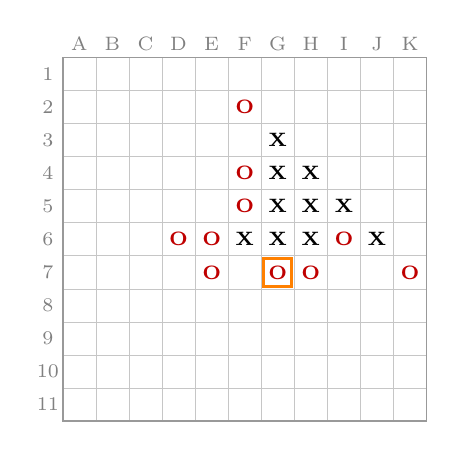
\begin{tikzpicture}[x=.42cm, y=.42cm]
\draw[gray!45, line width=.25pt] (0,0) -- (11,0);
\draw[gray!45, line width=.25pt] (0,0) -- (0,-11);
\draw[gray!45, line width=.25pt] (0,-1) -- (11,-1);
\draw[gray!45, line width=.25pt] (1,0) -- (1,-11);
\draw[gray!45, line width=.25pt] (0,-2) -- (11,-2);
\draw[gray!45, line width=.25pt] (2,0) -- (2,-11);
\draw[gray!45, line width=.25pt] (0,-3) -- (11,-3);
\draw[gray!45, line width=.25pt] (3,0) -- (3,-11);
\draw[gray!45, line width=.25pt] (0,-4) -- (11,-4);
\draw[gray!45, line width=.25pt] (4,0) -- (4,-11);
\draw[gray!45, line width=.25pt] (0,-5) -- (11,-5);
\draw[gray!45, line width=.25pt] (5,0) -- (5,-11);
\draw[gray!45, line width=.25pt] (0,-6) -- (11,-6);
\draw[gray!45, line width=.25pt] (6,0) -- (6,-11);
\draw[gray!45, line width=.25pt] (0,-7) -- (11,-7);
\draw[gray!45, line width=.25pt] (7,0) -- (7,-11);
\draw[gray!45, line width=.25pt] (0,-8) -- (11,-8);
\draw[gray!45, line width=.25pt] (8,0) -- (8,-11);
\draw[gray!45, line width=.25pt] (0,-9) -- (11,-9);
\draw[gray!45, line width=.25pt] (9,0) -- (9,-11);
\draw[gray!45, line width=.25pt] (0,-10) -- (11,-10);
\draw[gray!45, line width=.25pt] (10,0) -- (10,-11);
\draw[gray!45, line width=.25pt] (0,-11) -- (11,-11);
\draw[gray!45, line width=.25pt] (11,0) -- (11,-11);
\draw[gray!80, line width=.5pt] (0,0) rectangle (11,-11);
\node[font=\scriptsize, text=gray] at (0.5,.42) {A};
\node[font=\scriptsize, text=gray] at (1.5,.42) {B};
\node[font=\scriptsize, text=gray] at (2.5,.42) {C};
\node[font=\scriptsize, text=gray] at (3.5,.42) {D};
\node[font=\scriptsize, text=gray] at (4.5,.42) {E};
\node[font=\scriptsize, text=gray] at (5.5,.42) {F};
\node[font=\scriptsize, text=gray] at (6.5,.42) {G};
\node[font=\scriptsize, text=gray] at (7.5,.42) {H};
\node[font=\scriptsize, text=gray] at (8.5,.42) {I};
\node[font=\scriptsize, text=gray] at (9.5,.42) {J};
\node[font=\scriptsize, text=gray] at (10.5,.42) {K};
\node[font=\scriptsize, text=gray] at (-.45,-0.5) {1};
\node[font=\scriptsize, text=gray] at (-.45,-1.5) {2};
\node[font=\scriptsize, text=gray] at (-.45,-2.5) {3};
\node[font=\scriptsize, text=gray] at (-.45,-3.5) {4};
\node[font=\scriptsize, text=gray] at (-.45,-4.5) {5};
\node[font=\scriptsize, text=gray] at (-.45,-5.5) {6};
\node[font=\scriptsize, text=gray] at (-.45,-6.5) {7};
\node[font=\scriptsize, text=gray] at (-.45,-7.5) {8};
\node[font=\scriptsize, text=gray] at (-.45,-8.5) {9};
\node[font=\scriptsize, text=gray] at (-.45,-9.5) {10};
\node[font=\scriptsize, text=gray] at (-.45,-10.5) {11};
\node[text=red!75!black, font=\bfseries\scriptsize] at (5.5,-1.5) {O};
\node[text=black, font=\bfseries\scriptsize] at (6.5,-2.5) {X};
\node[text=red!75!black, font=\bfseries\scriptsize] at (5.5,-3.5) {O};
\node[text=black, font=\bfseries\scriptsize] at (6.5,-3.5) {X};
\node[text=black, font=\bfseries\scriptsize] at (7.5,-3.5) {X};
\node[text=red!75!black, font=\bfseries\scriptsize] at (5.5,-4.5) {O};
\node[text=black, font=\bfseries\scriptsize] at (6.5,-4.5) {X};
\node[text=black, font=\bfseries\scriptsize] at (7.5,-4.5) {X};
\node[text=black, font=\bfseries\scriptsize] at (8.5,-4.5) {X};
\node[text=red!75!black, font=\bfseries\scriptsize] at (3.5,-5.5) {O};
\node[text=red!75!black, font=\bfseries\scriptsize] at (4.5,-5.5) {O};
\node[text=black, font=\bfseries\scriptsize] at (5.5,-5.5) {X};
\node[text=black, font=\bfseries\scriptsize] at (6.5,-5.5) {X};
\node[text=black, font=\bfseries\scriptsize] at (7.5,-5.5) {X};
\node[text=red!75!black, font=\bfseries\scriptsize] at (8.5,-5.5) {O};
\node[text=black, font=\bfseries\scriptsize] at (9.5,-5.5) {X};
\node[text=red!75!black, font=\bfseries\scriptsize] at (4.5,-6.5) {O};
\node[text=red!75!black, font=\bfseries\scriptsize] at (6.5,-6.5) {O};
\draw[orange, line width=1pt] (6.08,-6.08) rectangle ++(.84,-.84);
\node[text=red!75!black, font=\bfseries\scriptsize] at (7.5,-6.5) {O};
\node[text=red!75!black, font=\bfseries\scriptsize] at (10.5,-6.5) {O};
\end{tikzpicture}
\end{center}
\paragraph{Thế kết thúc}
\begin{center}
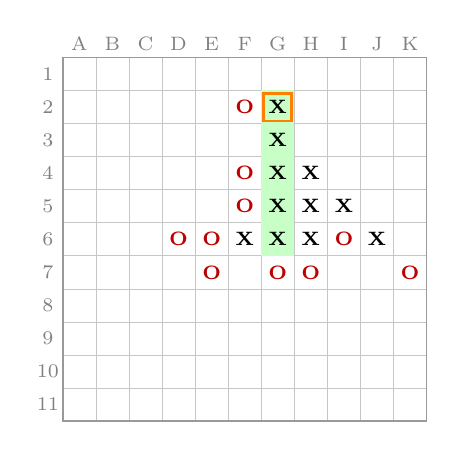
\begin{tikzpicture}[x=.42cm, y=.42cm]
\draw[gray!45, line width=.25pt] (0,0) -- (11,0);
\draw[gray!45, line width=.25pt] (0,0) -- (0,-11);
\draw[gray!45, line width=.25pt] (0,-1) -- (11,-1);
\draw[gray!45, line width=.25pt] (1,0) -- (1,-11);
\draw[gray!45, line width=.25pt] (0,-2) -- (11,-2);
\draw[gray!45, line width=.25pt] (2,0) -- (2,-11);
\draw[gray!45, line width=.25pt] (0,-3) -- (11,-3);
\draw[gray!45, line width=.25pt] (3,0) -- (3,-11);
\draw[gray!45, line width=.25pt] (0,-4) -- (11,-4);
\draw[gray!45, line width=.25pt] (4,0) -- (4,-11);
\draw[gray!45, line width=.25pt] (0,-5) -- (11,-5);
\draw[gray!45, line width=.25pt] (5,0) -- (5,-11);
\draw[gray!45, line width=.25pt] (0,-6) -- (11,-6);
\draw[gray!45, line width=.25pt] (6,0) -- (6,-11);
\draw[gray!45, line width=.25pt] (0,-7) -- (11,-7);
\draw[gray!45, line width=.25pt] (7,0) -- (7,-11);
\draw[gray!45, line width=.25pt] (0,-8) -- (11,-8);
\draw[gray!45, line width=.25pt] (8,0) -- (8,-11);
\draw[gray!45, line width=.25pt] (0,-9) -- (11,-9);
\draw[gray!45, line width=.25pt] (9,0) -- (9,-11);
\draw[gray!45, line width=.25pt] (0,-10) -- (11,-10);
\draw[gray!45, line width=.25pt] (10,0) -- (10,-11);
\draw[gray!45, line width=.25pt] (0,-11) -- (11,-11);
\draw[gray!45, line width=.25pt] (11,0) -- (11,-11);
\draw[gray!80, line width=.5pt] (0,0) rectangle (11,-11);
\node[font=\scriptsize, text=gray] at (0.5,.42) {A};
\node[font=\scriptsize, text=gray] at (1.5,.42) {B};
\node[font=\scriptsize, text=gray] at (2.5,.42) {C};
\node[font=\scriptsize, text=gray] at (3.5,.42) {D};
\node[font=\scriptsize, text=gray] at (4.5,.42) {E};
\node[font=\scriptsize, text=gray] at (5.5,.42) {F};
\node[font=\scriptsize, text=gray] at (6.5,.42) {G};
\node[font=\scriptsize, text=gray] at (7.5,.42) {H};
\node[font=\scriptsize, text=gray] at (8.5,.42) {I};
\node[font=\scriptsize, text=gray] at (9.5,.42) {J};
\node[font=\scriptsize, text=gray] at (10.5,.42) {K};
\node[font=\scriptsize, text=gray] at (-.45,-0.5) {1};
\node[font=\scriptsize, text=gray] at (-.45,-1.5) {2};
\node[font=\scriptsize, text=gray] at (-.45,-2.5) {3};
\node[font=\scriptsize, text=gray] at (-.45,-3.5) {4};
\node[font=\scriptsize, text=gray] at (-.45,-4.5) {5};
\node[font=\scriptsize, text=gray] at (-.45,-5.5) {6};
\node[font=\scriptsize, text=gray] at (-.45,-6.5) {7};
\node[font=\scriptsize, text=gray] at (-.45,-7.5) {8};
\node[font=\scriptsize, text=gray] at (-.45,-8.5) {9};
\node[font=\scriptsize, text=gray] at (-.45,-9.5) {10};
\node[font=\scriptsize, text=gray] at (-.45,-10.5) {11};
\node[text=red!75!black, font=\bfseries\scriptsize] at (5.5,-1.5) {O};
\fill[green!22] (6,-1) rectangle ++(1,-1);
\node[text=black, font=\bfseries\scriptsize] at (6.5,-1.5) {X};
\draw[orange, line width=1pt] (6.08,-1.08) rectangle ++(.84,-.84);
\fill[green!22] (6,-2) rectangle ++(1,-1);
\node[text=black, font=\bfseries\scriptsize] at (6.5,-2.5) {X};
\node[text=red!75!black, font=\bfseries\scriptsize] at (5.5,-3.5) {O};
\fill[green!22] (6,-3) rectangle ++(1,-1);
\node[text=black, font=\bfseries\scriptsize] at (6.5,-3.5) {X};
\node[text=black, font=\bfseries\scriptsize] at (7.5,-3.5) {X};
\node[text=red!75!black, font=\bfseries\scriptsize] at (5.5,-4.5) {O};
\fill[green!22] (6,-4) rectangle ++(1,-1);
\node[text=black, font=\bfseries\scriptsize] at (6.5,-4.5) {X};
\node[text=black, font=\bfseries\scriptsize] at (7.5,-4.5) {X};
\node[text=black, font=\bfseries\scriptsize] at (8.5,-4.5) {X};
\node[text=red!75!black, font=\bfseries\scriptsize] at (3.5,-5.5) {O};
\node[text=red!75!black, font=\bfseries\scriptsize] at (4.5,-5.5) {O};
\node[text=black, font=\bfseries\scriptsize] at (5.5,-5.5) {X};
\fill[green!22] (6,-5) rectangle ++(1,-1);
\node[text=black, font=\bfseries\scriptsize] at (6.5,-5.5) {X};
\node[text=black, font=\bfseries\scriptsize] at (7.5,-5.5) {X};
\node[text=red!75!black, font=\bfseries\scriptsize] at (8.5,-5.5) {O};
\node[text=black, font=\bfseries\scriptsize] at (9.5,-5.5) {X};
\node[text=red!75!black, font=\bfseries\scriptsize] at (4.5,-6.5) {O};
\node[text=red!75!black, font=\bfseries\scriptsize] at (6.5,-6.5) {O};
\node[text=red!75!black, font=\bfseries\scriptsize] at (7.5,-6.5) {O};
\node[text=red!75!black, font=\bfseries\scriptsize] at (10.5,-6.5) {O};
\end{tikzpicture}
\end{center}
\paragraph{Cơ chế kết thúc} Trước nước áp chót, bên thắng đã có 2 ô thắng ngay (G2, G7); đối thủ chỉ chặn được một ô, nên nước G2 hoàn thành dãy năm quân.
\paragraph{Nhận xét} L7 cầm X thắng L8 trong 21 nước bằng cột G. Trước nước 20, X có bốn quân G3–G6; hai đầu G2 và G7 là ô thắng. O chặn G7, X đi G2. Ván này giống ván 07 ở chỗ đòn kép hai đầu quyết định, nhưng bên thắng là L7 và bên thua là L8. Nó cho thấy L8 không miễn nhiễm với đe doạ dọc.
\paragraph{Diễn biến} {\footnotesize 1.H6 2.E6 3.F6 4.D6 5.G5 6.F4 7.H4 8.E7 9.H5 10.H7 11.I5 12.F5 13.G3 14.F2 15.J6 16.K7 17.G6 18.I6 19.G4 20.G7 21.G2\par}

\subsection{L7–L8 · ván 15}
Khai cuộc gồm 2 nước: G6 → D4. X: \texttt{L7-PUCT[l5]}, O: \texttt{L8}. Kết quả: O thắng sau 58 nước.
\begin{center}\small
\begin{tabular}{@{}rccll@{}}
\toprule
Ply & Màu & Nước & Nhận xét & Ô liên quan \\
\midrule
28 & O & A7 & Chặn bắt buộc & A7 \\
36 & O & I1 & Chặn bắt buộc & I1 \\
48 & O & K8 & Chặn bắt buộc & K8 \\
51 & X & H7 & Chặn bắt buộc & H7 \\
53 & X & F2 & Chặn bắt buộc & F2 \\
55 & X & J2 & Chặn bắt buộc & J2 \\
\bottomrule
\end{tabular}
\end{center}
\paragraph{Thế cờ trước nước quyết định (sau nước 54)}
\begin{center}
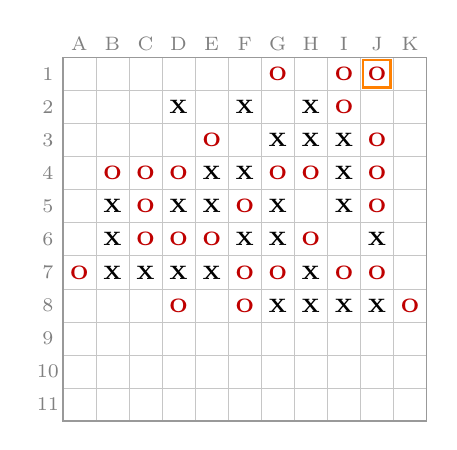
\begin{tikzpicture}[x=.42cm, y=.42cm]
\draw[gray!45, line width=.25pt] (0,0) -- (11,0);
\draw[gray!45, line width=.25pt] (0,0) -- (0,-11);
\draw[gray!45, line width=.25pt] (0,-1) -- (11,-1);
\draw[gray!45, line width=.25pt] (1,0) -- (1,-11);
\draw[gray!45, line width=.25pt] (0,-2) -- (11,-2);
\draw[gray!45, line width=.25pt] (2,0) -- (2,-11);
\draw[gray!45, line width=.25pt] (0,-3) -- (11,-3);
\draw[gray!45, line width=.25pt] (3,0) -- (3,-11);
\draw[gray!45, line width=.25pt] (0,-4) -- (11,-4);
\draw[gray!45, line width=.25pt] (4,0) -- (4,-11);
\draw[gray!45, line width=.25pt] (0,-5) -- (11,-5);
\draw[gray!45, line width=.25pt] (5,0) -- (5,-11);
\draw[gray!45, line width=.25pt] (0,-6) -- (11,-6);
\draw[gray!45, line width=.25pt] (6,0) -- (6,-11);
\draw[gray!45, line width=.25pt] (0,-7) -- (11,-7);
\draw[gray!45, line width=.25pt] (7,0) -- (7,-11);
\draw[gray!45, line width=.25pt] (0,-8) -- (11,-8);
\draw[gray!45, line width=.25pt] (8,0) -- (8,-11);
\draw[gray!45, line width=.25pt] (0,-9) -- (11,-9);
\draw[gray!45, line width=.25pt] (9,0) -- (9,-11);
\draw[gray!45, line width=.25pt] (0,-10) -- (11,-10);
\draw[gray!45, line width=.25pt] (10,0) -- (10,-11);
\draw[gray!45, line width=.25pt] (0,-11) -- (11,-11);
\draw[gray!45, line width=.25pt] (11,0) -- (11,-11);
\draw[gray!80, line width=.5pt] (0,0) rectangle (11,-11);
\node[font=\scriptsize, text=gray] at (0.5,.42) {A};
\node[font=\scriptsize, text=gray] at (1.5,.42) {B};
\node[font=\scriptsize, text=gray] at (2.5,.42) {C};
\node[font=\scriptsize, text=gray] at (3.5,.42) {D};
\node[font=\scriptsize, text=gray] at (4.5,.42) {E};
\node[font=\scriptsize, text=gray] at (5.5,.42) {F};
\node[font=\scriptsize, text=gray] at (6.5,.42) {G};
\node[font=\scriptsize, text=gray] at (7.5,.42) {H};
\node[font=\scriptsize, text=gray] at (8.5,.42) {I};
\node[font=\scriptsize, text=gray] at (9.5,.42) {J};
\node[font=\scriptsize, text=gray] at (10.5,.42) {K};
\node[font=\scriptsize, text=gray] at (-.45,-0.5) {1};
\node[font=\scriptsize, text=gray] at (-.45,-1.5) {2};
\node[font=\scriptsize, text=gray] at (-.45,-2.5) {3};
\node[font=\scriptsize, text=gray] at (-.45,-3.5) {4};
\node[font=\scriptsize, text=gray] at (-.45,-4.5) {5};
\node[font=\scriptsize, text=gray] at (-.45,-5.5) {6};
\node[font=\scriptsize, text=gray] at (-.45,-6.5) {7};
\node[font=\scriptsize, text=gray] at (-.45,-7.5) {8};
\node[font=\scriptsize, text=gray] at (-.45,-8.5) {9};
\node[font=\scriptsize, text=gray] at (-.45,-9.5) {10};
\node[font=\scriptsize, text=gray] at (-.45,-10.5) {11};
\node[text=red!75!black, font=\bfseries\scriptsize] at (6.5,-0.5) {O};
\node[text=red!75!black, font=\bfseries\scriptsize] at (8.5,-0.5) {O};
\node[text=red!75!black, font=\bfseries\scriptsize] at (9.5,-0.5) {O};
\draw[orange, line width=1pt] (9.08,-0.08) rectangle ++(.84,-.84);
\node[text=black, font=\bfseries\scriptsize] at (3.5,-1.5) {X};
\node[text=black, font=\bfseries\scriptsize] at (5.5,-1.5) {X};
\node[text=black, font=\bfseries\scriptsize] at (7.5,-1.5) {X};
\node[text=red!75!black, font=\bfseries\scriptsize] at (8.5,-1.5) {O};
\node[text=red!75!black, font=\bfseries\scriptsize] at (4.5,-2.5) {O};
\node[text=black, font=\bfseries\scriptsize] at (6.5,-2.5) {X};
\node[text=black, font=\bfseries\scriptsize] at (7.5,-2.5) {X};
\node[text=black, font=\bfseries\scriptsize] at (8.5,-2.5) {X};
\node[text=red!75!black, font=\bfseries\scriptsize] at (9.5,-2.5) {O};
\node[text=red!75!black, font=\bfseries\scriptsize] at (1.5,-3.5) {O};
\node[text=red!75!black, font=\bfseries\scriptsize] at (2.5,-3.5) {O};
\node[text=red!75!black, font=\bfseries\scriptsize] at (3.5,-3.5) {O};
\node[text=black, font=\bfseries\scriptsize] at (4.5,-3.5) {X};
\node[text=black, font=\bfseries\scriptsize] at (5.5,-3.5) {X};
\node[text=red!75!black, font=\bfseries\scriptsize] at (6.5,-3.5) {O};
\node[text=red!75!black, font=\bfseries\scriptsize] at (7.5,-3.5) {O};
\node[text=black, font=\bfseries\scriptsize] at (8.5,-3.5) {X};
\node[text=red!75!black, font=\bfseries\scriptsize] at (9.5,-3.5) {O};
\node[text=black, font=\bfseries\scriptsize] at (1.5,-4.5) {X};
\node[text=red!75!black, font=\bfseries\scriptsize] at (2.5,-4.5) {O};
\node[text=black, font=\bfseries\scriptsize] at (3.5,-4.5) {X};
\node[text=black, font=\bfseries\scriptsize] at (4.5,-4.5) {X};
\node[text=red!75!black, font=\bfseries\scriptsize] at (5.5,-4.5) {O};
\node[text=black, font=\bfseries\scriptsize] at (6.5,-4.5) {X};
\node[text=black, font=\bfseries\scriptsize] at (8.5,-4.5) {X};
\node[text=red!75!black, font=\bfseries\scriptsize] at (9.5,-4.5) {O};
\node[text=black, font=\bfseries\scriptsize] at (1.5,-5.5) {X};
\node[text=red!75!black, font=\bfseries\scriptsize] at (2.5,-5.5) {O};
\node[text=red!75!black, font=\bfseries\scriptsize] at (3.5,-5.5) {O};
\node[text=red!75!black, font=\bfseries\scriptsize] at (4.5,-5.5) {O};
\node[text=black, font=\bfseries\scriptsize] at (5.5,-5.5) {X};
\node[text=black, font=\bfseries\scriptsize] at (6.5,-5.5) {X};
\node[text=red!75!black, font=\bfseries\scriptsize] at (7.5,-5.5) {O};
\node[text=black, font=\bfseries\scriptsize] at (9.5,-5.5) {X};
\node[text=red!75!black, font=\bfseries\scriptsize] at (0.5,-6.5) {O};
\node[text=black, font=\bfseries\scriptsize] at (1.5,-6.5) {X};
\node[text=black, font=\bfseries\scriptsize] at (2.5,-6.5) {X};
\node[text=black, font=\bfseries\scriptsize] at (3.5,-6.5) {X};
\node[text=black, font=\bfseries\scriptsize] at (4.5,-6.5) {X};
\node[text=red!75!black, font=\bfseries\scriptsize] at (5.5,-6.5) {O};
\node[text=red!75!black, font=\bfseries\scriptsize] at (6.5,-6.5) {O};
\node[text=black, font=\bfseries\scriptsize] at (7.5,-6.5) {X};
\node[text=red!75!black, font=\bfseries\scriptsize] at (8.5,-6.5) {O};
\node[text=red!75!black, font=\bfseries\scriptsize] at (9.5,-6.5) {O};
\node[text=red!75!black, font=\bfseries\scriptsize] at (3.5,-7.5) {O};
\node[text=red!75!black, font=\bfseries\scriptsize] at (5.5,-7.5) {O};
\node[text=black, font=\bfseries\scriptsize] at (6.5,-7.5) {X};
\node[text=black, font=\bfseries\scriptsize] at (7.5,-7.5) {X};
\node[text=black, font=\bfseries\scriptsize] at (8.5,-7.5) {X};
\node[text=black, font=\bfseries\scriptsize] at (9.5,-7.5) {X};
\node[text=red!75!black, font=\bfseries\scriptsize] at (10.5,-7.5) {O};
\end{tikzpicture}
\end{center}
\paragraph{Thế kết thúc}
\begin{center}
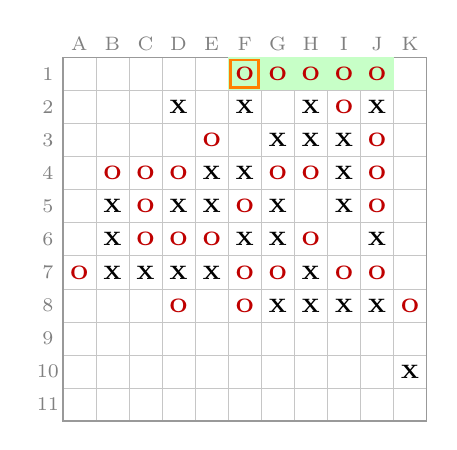
\begin{tikzpicture}[x=.42cm, y=.42cm]
\draw[gray!45, line width=.25pt] (0,0) -- (11,0);
\draw[gray!45, line width=.25pt] (0,0) -- (0,-11);
\draw[gray!45, line width=.25pt] (0,-1) -- (11,-1);
\draw[gray!45, line width=.25pt] (1,0) -- (1,-11);
\draw[gray!45, line width=.25pt] (0,-2) -- (11,-2);
\draw[gray!45, line width=.25pt] (2,0) -- (2,-11);
\draw[gray!45, line width=.25pt] (0,-3) -- (11,-3);
\draw[gray!45, line width=.25pt] (3,0) -- (3,-11);
\draw[gray!45, line width=.25pt] (0,-4) -- (11,-4);
\draw[gray!45, line width=.25pt] (4,0) -- (4,-11);
\draw[gray!45, line width=.25pt] (0,-5) -- (11,-5);
\draw[gray!45, line width=.25pt] (5,0) -- (5,-11);
\draw[gray!45, line width=.25pt] (0,-6) -- (11,-6);
\draw[gray!45, line width=.25pt] (6,0) -- (6,-11);
\draw[gray!45, line width=.25pt] (0,-7) -- (11,-7);
\draw[gray!45, line width=.25pt] (7,0) -- (7,-11);
\draw[gray!45, line width=.25pt] (0,-8) -- (11,-8);
\draw[gray!45, line width=.25pt] (8,0) -- (8,-11);
\draw[gray!45, line width=.25pt] (0,-9) -- (11,-9);
\draw[gray!45, line width=.25pt] (9,0) -- (9,-11);
\draw[gray!45, line width=.25pt] (0,-10) -- (11,-10);
\draw[gray!45, line width=.25pt] (10,0) -- (10,-11);
\draw[gray!45, line width=.25pt] (0,-11) -- (11,-11);
\draw[gray!45, line width=.25pt] (11,0) -- (11,-11);
\draw[gray!80, line width=.5pt] (0,0) rectangle (11,-11);
\node[font=\scriptsize, text=gray] at (0.5,.42) {A};
\node[font=\scriptsize, text=gray] at (1.5,.42) {B};
\node[font=\scriptsize, text=gray] at (2.5,.42) {C};
\node[font=\scriptsize, text=gray] at (3.5,.42) {D};
\node[font=\scriptsize, text=gray] at (4.5,.42) {E};
\node[font=\scriptsize, text=gray] at (5.5,.42) {F};
\node[font=\scriptsize, text=gray] at (6.5,.42) {G};
\node[font=\scriptsize, text=gray] at (7.5,.42) {H};
\node[font=\scriptsize, text=gray] at (8.5,.42) {I};
\node[font=\scriptsize, text=gray] at (9.5,.42) {J};
\node[font=\scriptsize, text=gray] at (10.5,.42) {K};
\node[font=\scriptsize, text=gray] at (-.45,-0.5) {1};
\node[font=\scriptsize, text=gray] at (-.45,-1.5) {2};
\node[font=\scriptsize, text=gray] at (-.45,-2.5) {3};
\node[font=\scriptsize, text=gray] at (-.45,-3.5) {4};
\node[font=\scriptsize, text=gray] at (-.45,-4.5) {5};
\node[font=\scriptsize, text=gray] at (-.45,-5.5) {6};
\node[font=\scriptsize, text=gray] at (-.45,-6.5) {7};
\node[font=\scriptsize, text=gray] at (-.45,-7.5) {8};
\node[font=\scriptsize, text=gray] at (-.45,-8.5) {9};
\node[font=\scriptsize, text=gray] at (-.45,-9.5) {10};
\node[font=\scriptsize, text=gray] at (-.45,-10.5) {11};
\fill[green!22] (5,0) rectangle ++(1,-1);
\node[text=red!75!black, font=\bfseries\scriptsize] at (5.5,-0.5) {O};
\draw[orange, line width=1pt] (5.08,-0.08) rectangle ++(.84,-.84);
\fill[green!22] (6,0) rectangle ++(1,-1);
\node[text=red!75!black, font=\bfseries\scriptsize] at (6.5,-0.5) {O};
\fill[green!22] (7,0) rectangle ++(1,-1);
\node[text=red!75!black, font=\bfseries\scriptsize] at (7.5,-0.5) {O};
\fill[green!22] (8,0) rectangle ++(1,-1);
\node[text=red!75!black, font=\bfseries\scriptsize] at (8.5,-0.5) {O};
\fill[green!22] (9,0) rectangle ++(1,-1);
\node[text=red!75!black, font=\bfseries\scriptsize] at (9.5,-0.5) {O};
\node[text=black, font=\bfseries\scriptsize] at (3.5,-1.5) {X};
\node[text=black, font=\bfseries\scriptsize] at (5.5,-1.5) {X};
\node[text=black, font=\bfseries\scriptsize] at (7.5,-1.5) {X};
\node[text=red!75!black, font=\bfseries\scriptsize] at (8.5,-1.5) {O};
\node[text=black, font=\bfseries\scriptsize] at (9.5,-1.5) {X};
\node[text=red!75!black, font=\bfseries\scriptsize] at (4.5,-2.5) {O};
\node[text=black, font=\bfseries\scriptsize] at (6.5,-2.5) {X};
\node[text=black, font=\bfseries\scriptsize] at (7.5,-2.5) {X};
\node[text=black, font=\bfseries\scriptsize] at (8.5,-2.5) {X};
\node[text=red!75!black, font=\bfseries\scriptsize] at (9.5,-2.5) {O};
\node[text=red!75!black, font=\bfseries\scriptsize] at (1.5,-3.5) {O};
\node[text=red!75!black, font=\bfseries\scriptsize] at (2.5,-3.5) {O};
\node[text=red!75!black, font=\bfseries\scriptsize] at (3.5,-3.5) {O};
\node[text=black, font=\bfseries\scriptsize] at (4.5,-3.5) {X};
\node[text=black, font=\bfseries\scriptsize] at (5.5,-3.5) {X};
\node[text=red!75!black, font=\bfseries\scriptsize] at (6.5,-3.5) {O};
\node[text=red!75!black, font=\bfseries\scriptsize] at (7.5,-3.5) {O};
\node[text=black, font=\bfseries\scriptsize] at (8.5,-3.5) {X};
\node[text=red!75!black, font=\bfseries\scriptsize] at (9.5,-3.5) {O};
\node[text=black, font=\bfseries\scriptsize] at (1.5,-4.5) {X};
\node[text=red!75!black, font=\bfseries\scriptsize] at (2.5,-4.5) {O};
\node[text=black, font=\bfseries\scriptsize] at (3.5,-4.5) {X};
\node[text=black, font=\bfseries\scriptsize] at (4.5,-4.5) {X};
\node[text=red!75!black, font=\bfseries\scriptsize] at (5.5,-4.5) {O};
\node[text=black, font=\bfseries\scriptsize] at (6.5,-4.5) {X};
\node[text=black, font=\bfseries\scriptsize] at (8.5,-4.5) {X};
\node[text=red!75!black, font=\bfseries\scriptsize] at (9.5,-4.5) {O};
\node[text=black, font=\bfseries\scriptsize] at (1.5,-5.5) {X};
\node[text=red!75!black, font=\bfseries\scriptsize] at (2.5,-5.5) {O};
\node[text=red!75!black, font=\bfseries\scriptsize] at (3.5,-5.5) {O};
\node[text=red!75!black, font=\bfseries\scriptsize] at (4.5,-5.5) {O};
\node[text=black, font=\bfseries\scriptsize] at (5.5,-5.5) {X};
\node[text=black, font=\bfseries\scriptsize] at (6.5,-5.5) {X};
\node[text=red!75!black, font=\bfseries\scriptsize] at (7.5,-5.5) {O};
\node[text=black, font=\bfseries\scriptsize] at (9.5,-5.5) {X};
\node[text=red!75!black, font=\bfseries\scriptsize] at (0.5,-6.5) {O};
\node[text=black, font=\bfseries\scriptsize] at (1.5,-6.5) {X};
\node[text=black, font=\bfseries\scriptsize] at (2.5,-6.5) {X};
\node[text=black, font=\bfseries\scriptsize] at (3.5,-6.5) {X};
\node[text=black, font=\bfseries\scriptsize] at (4.5,-6.5) {X};
\node[text=red!75!black, font=\bfseries\scriptsize] at (5.5,-6.5) {O};
\node[text=red!75!black, font=\bfseries\scriptsize] at (6.5,-6.5) {O};
\node[text=black, font=\bfseries\scriptsize] at (7.5,-6.5) {X};
\node[text=red!75!black, font=\bfseries\scriptsize] at (8.5,-6.5) {O};
\node[text=red!75!black, font=\bfseries\scriptsize] at (9.5,-6.5) {O};
\node[text=red!75!black, font=\bfseries\scriptsize] at (3.5,-7.5) {O};
\node[text=red!75!black, font=\bfseries\scriptsize] at (5.5,-7.5) {O};
\node[text=black, font=\bfseries\scriptsize] at (6.5,-7.5) {X};
\node[text=black, font=\bfseries\scriptsize] at (7.5,-7.5) {X};
\node[text=black, font=\bfseries\scriptsize] at (8.5,-7.5) {X};
\node[text=black, font=\bfseries\scriptsize] at (9.5,-7.5) {X};
\node[text=red!75!black, font=\bfseries\scriptsize] at (10.5,-7.5) {O};
\node[text=black, font=\bfseries\scriptsize] at (10.5,-9.5) {X};
\end{tikzpicture}
\end{center}
\paragraph{Cơ chế kết thúc} Trước nước áp chót, bên thắng đã có 2 ô thắng ngay (F1, K1); đối thủ chỉ chặn được một ô, nên nước F1 hoàn thành dãy năm quân.
\paragraph{Nhận xét} L8 cầm O thắng L7 sau 58 nước bằng hàng ngang F1–J1. Trước nước 58, O có bốn quân G1–J1; hai đầu F1 và K1 là ô thắng. X đi K10, O đi F1. Ván dài, nhiều nước đổi cánh, nhưng cơ chế kết thúc vẫn là đòn kép hai đầu. Đây là ví dụ L8 cầm O thắng L7, góp phần vào 82,5\% điểm của L8 trước L7.
\paragraph{Diễn biến} {\footnotesize 1.G6 2.D4 3.G5 4.G4 5.F6 6.E6 7.E7 8.H4 9.F4 10.F5 11.D7 12.H6 13.H3 14.F7 15.G8 16.D8 17.G3 18.G7 19.D2 20.E3 21.E5 22.D6 23.I3 24.J3 25.B7 26.J4 27.C7 28.A7 29.I5 30.J5 31.J6 32.C4 33.I4 34.I2 35.H2 36.I1 37.D5 38.C6 39.B6 40.B4 41.B5 42.C5 43.H8 44.I7 45.I8 46.F8 47.J8 48.K8 49.E4 50.J7 51.H7 52.G1 53.F2 54.J1 55.J2 56.H1 57.K10 58.F1\par}

\subsection{RR8 · L4 thua L2 · ván 1101}
Khai cuộc gồm 4 nước: H8 → D6 → G5 → H6. X: \texttt{L4-MCTS}, O: \texttt{L2-Rule}. Kết quả: O thắng sau 12 nước.
\begin{center}\small
\begin{tabular}{@{}rccll@{}}
\toprule
Ply & Màu & Nước & Nhận xét & Ô liên quan \\
\midrule
9 & X & G6 & Chặn bắt buộc & G6 \\
11 & X & C1 & Bỏ chặn duy nhất & B6 \\
12 & O & B6 & Thắng ngay & — \\
\bottomrule
\end{tabular}
\end{center}
\paragraph{Thế cờ trước nước quyết định (sau nước 11)}
\begin{center}
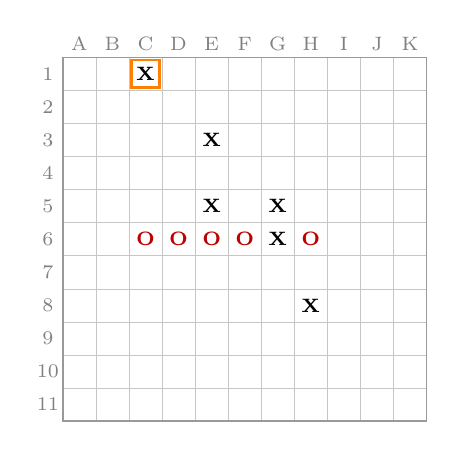
\begin{tikzpicture}[x=.42cm, y=.42cm]
\draw[gray!45, line width=.25pt] (0,0) -- (11,0);
\draw[gray!45, line width=.25pt] (0,0) -- (0,-11);
\draw[gray!45, line width=.25pt] (0,-1) -- (11,-1);
\draw[gray!45, line width=.25pt] (1,0) -- (1,-11);
\draw[gray!45, line width=.25pt] (0,-2) -- (11,-2);
\draw[gray!45, line width=.25pt] (2,0) -- (2,-11);
\draw[gray!45, line width=.25pt] (0,-3) -- (11,-3);
\draw[gray!45, line width=.25pt] (3,0) -- (3,-11);
\draw[gray!45, line width=.25pt] (0,-4) -- (11,-4);
\draw[gray!45, line width=.25pt] (4,0) -- (4,-11);
\draw[gray!45, line width=.25pt] (0,-5) -- (11,-5);
\draw[gray!45, line width=.25pt] (5,0) -- (5,-11);
\draw[gray!45, line width=.25pt] (0,-6) -- (11,-6);
\draw[gray!45, line width=.25pt] (6,0) -- (6,-11);
\draw[gray!45, line width=.25pt] (0,-7) -- (11,-7);
\draw[gray!45, line width=.25pt] (7,0) -- (7,-11);
\draw[gray!45, line width=.25pt] (0,-8) -- (11,-8);
\draw[gray!45, line width=.25pt] (8,0) -- (8,-11);
\draw[gray!45, line width=.25pt] (0,-9) -- (11,-9);
\draw[gray!45, line width=.25pt] (9,0) -- (9,-11);
\draw[gray!45, line width=.25pt] (0,-10) -- (11,-10);
\draw[gray!45, line width=.25pt] (10,0) -- (10,-11);
\draw[gray!45, line width=.25pt] (0,-11) -- (11,-11);
\draw[gray!45, line width=.25pt] (11,0) -- (11,-11);
\draw[gray!80, line width=.5pt] (0,0) rectangle (11,-11);
\node[font=\scriptsize, text=gray] at (0.5,.42) {A};
\node[font=\scriptsize, text=gray] at (1.5,.42) {B};
\node[font=\scriptsize, text=gray] at (2.5,.42) {C};
\node[font=\scriptsize, text=gray] at (3.5,.42) {D};
\node[font=\scriptsize, text=gray] at (4.5,.42) {E};
\node[font=\scriptsize, text=gray] at (5.5,.42) {F};
\node[font=\scriptsize, text=gray] at (6.5,.42) {G};
\node[font=\scriptsize, text=gray] at (7.5,.42) {H};
\node[font=\scriptsize, text=gray] at (8.5,.42) {I};
\node[font=\scriptsize, text=gray] at (9.5,.42) {J};
\node[font=\scriptsize, text=gray] at (10.5,.42) {K};
\node[font=\scriptsize, text=gray] at (-.45,-0.5) {1};
\node[font=\scriptsize, text=gray] at (-.45,-1.5) {2};
\node[font=\scriptsize, text=gray] at (-.45,-2.5) {3};
\node[font=\scriptsize, text=gray] at (-.45,-3.5) {4};
\node[font=\scriptsize, text=gray] at (-.45,-4.5) {5};
\node[font=\scriptsize, text=gray] at (-.45,-5.5) {6};
\node[font=\scriptsize, text=gray] at (-.45,-6.5) {7};
\node[font=\scriptsize, text=gray] at (-.45,-7.5) {8};
\node[font=\scriptsize, text=gray] at (-.45,-8.5) {9};
\node[font=\scriptsize, text=gray] at (-.45,-9.5) {10};
\node[font=\scriptsize, text=gray] at (-.45,-10.5) {11};
\node[text=black, font=\bfseries\scriptsize] at (2.5,-0.5) {X};
\draw[orange, line width=1pt] (2.08,-0.08) rectangle ++(.84,-.84);
\node[text=black, font=\bfseries\scriptsize] at (4.5,-2.5) {X};
\node[text=black, font=\bfseries\scriptsize] at (4.5,-4.5) {X};
\node[text=black, font=\bfseries\scriptsize] at (6.5,-4.5) {X};
\node[text=red!75!black, font=\bfseries\scriptsize] at (2.5,-5.5) {O};
\node[text=red!75!black, font=\bfseries\scriptsize] at (3.5,-5.5) {O};
\node[text=red!75!black, font=\bfseries\scriptsize] at (4.5,-5.5) {O};
\node[text=red!75!black, font=\bfseries\scriptsize] at (5.5,-5.5) {O};
\node[text=black, font=\bfseries\scriptsize] at (6.5,-5.5) {X};
\node[text=red!75!black, font=\bfseries\scriptsize] at (7.5,-5.5) {O};
\node[text=black, font=\bfseries\scriptsize] at (7.5,-7.5) {X};
\end{tikzpicture}
\end{center}
\paragraph{Thế kết thúc}
\begin{center}
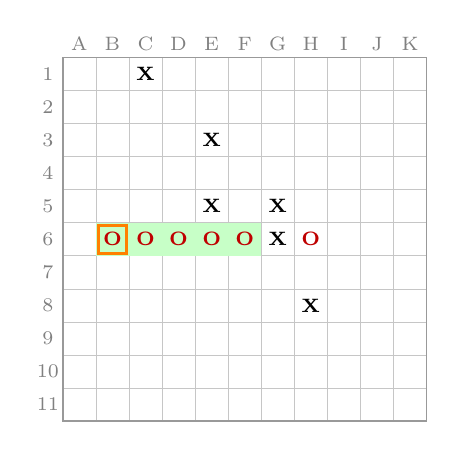
\begin{tikzpicture}[x=.42cm, y=.42cm]
\draw[gray!45, line width=.25pt] (0,0) -- (11,0);
\draw[gray!45, line width=.25pt] (0,0) -- (0,-11);
\draw[gray!45, line width=.25pt] (0,-1) -- (11,-1);
\draw[gray!45, line width=.25pt] (1,0) -- (1,-11);
\draw[gray!45, line width=.25pt] (0,-2) -- (11,-2);
\draw[gray!45, line width=.25pt] (2,0) -- (2,-11);
\draw[gray!45, line width=.25pt] (0,-3) -- (11,-3);
\draw[gray!45, line width=.25pt] (3,0) -- (3,-11);
\draw[gray!45, line width=.25pt] (0,-4) -- (11,-4);
\draw[gray!45, line width=.25pt] (4,0) -- (4,-11);
\draw[gray!45, line width=.25pt] (0,-5) -- (11,-5);
\draw[gray!45, line width=.25pt] (5,0) -- (5,-11);
\draw[gray!45, line width=.25pt] (0,-6) -- (11,-6);
\draw[gray!45, line width=.25pt] (6,0) -- (6,-11);
\draw[gray!45, line width=.25pt] (0,-7) -- (11,-7);
\draw[gray!45, line width=.25pt] (7,0) -- (7,-11);
\draw[gray!45, line width=.25pt] (0,-8) -- (11,-8);
\draw[gray!45, line width=.25pt] (8,0) -- (8,-11);
\draw[gray!45, line width=.25pt] (0,-9) -- (11,-9);
\draw[gray!45, line width=.25pt] (9,0) -- (9,-11);
\draw[gray!45, line width=.25pt] (0,-10) -- (11,-10);
\draw[gray!45, line width=.25pt] (10,0) -- (10,-11);
\draw[gray!45, line width=.25pt] (0,-11) -- (11,-11);
\draw[gray!45, line width=.25pt] (11,0) -- (11,-11);
\draw[gray!80, line width=.5pt] (0,0) rectangle (11,-11);
\node[font=\scriptsize, text=gray] at (0.5,.42) {A};
\node[font=\scriptsize, text=gray] at (1.5,.42) {B};
\node[font=\scriptsize, text=gray] at (2.5,.42) {C};
\node[font=\scriptsize, text=gray] at (3.5,.42) {D};
\node[font=\scriptsize, text=gray] at (4.5,.42) {E};
\node[font=\scriptsize, text=gray] at (5.5,.42) {F};
\node[font=\scriptsize, text=gray] at (6.5,.42) {G};
\node[font=\scriptsize, text=gray] at (7.5,.42) {H};
\node[font=\scriptsize, text=gray] at (8.5,.42) {I};
\node[font=\scriptsize, text=gray] at (9.5,.42) {J};
\node[font=\scriptsize, text=gray] at (10.5,.42) {K};
\node[font=\scriptsize, text=gray] at (-.45,-0.5) {1};
\node[font=\scriptsize, text=gray] at (-.45,-1.5) {2};
\node[font=\scriptsize, text=gray] at (-.45,-2.5) {3};
\node[font=\scriptsize, text=gray] at (-.45,-3.5) {4};
\node[font=\scriptsize, text=gray] at (-.45,-4.5) {5};
\node[font=\scriptsize, text=gray] at (-.45,-5.5) {6};
\node[font=\scriptsize, text=gray] at (-.45,-6.5) {7};
\node[font=\scriptsize, text=gray] at (-.45,-7.5) {8};
\node[font=\scriptsize, text=gray] at (-.45,-8.5) {9};
\node[font=\scriptsize, text=gray] at (-.45,-9.5) {10};
\node[font=\scriptsize, text=gray] at (-.45,-10.5) {11};
\node[text=black, font=\bfseries\scriptsize] at (2.5,-0.5) {X};
\node[text=black, font=\bfseries\scriptsize] at (4.5,-2.5) {X};
\node[text=black, font=\bfseries\scriptsize] at (4.5,-4.5) {X};
\node[text=black, font=\bfseries\scriptsize] at (6.5,-4.5) {X};
\fill[green!22] (1,-5) rectangle ++(1,-1);
\node[text=red!75!black, font=\bfseries\scriptsize] at (1.5,-5.5) {O};
\draw[orange, line width=1pt] (1.08,-5.08) rectangle ++(.84,-.84);
\fill[green!22] (2,-5) rectangle ++(1,-1);
\node[text=red!75!black, font=\bfseries\scriptsize] at (2.5,-5.5) {O};
\fill[green!22] (3,-5) rectangle ++(1,-1);
\node[text=red!75!black, font=\bfseries\scriptsize] at (3.5,-5.5) {O};
\fill[green!22] (4,-5) rectangle ++(1,-1);
\node[text=red!75!black, font=\bfseries\scriptsize] at (4.5,-5.5) {O};
\fill[green!22] (5,-5) rectangle ++(1,-1);
\node[text=red!75!black, font=\bfseries\scriptsize] at (5.5,-5.5) {O};
\node[text=black, font=\bfseries\scriptsize] at (6.5,-5.5) {X};
\node[text=red!75!black, font=\bfseries\scriptsize] at (7.5,-5.5) {O};
\node[text=black, font=\bfseries\scriptsize] at (7.5,-7.5) {X};
\end{tikzpicture}
\end{center}
\paragraph{Cơ chế kết thúc} Trước nước áp chót, bên thắng có đúng một ô thắng ngay (B6); đối thủ không chặn, nên nước B6 hoàn thành dãy.
\paragraph{Nhận xét} Ván ngắn nhất trong nhóm L4 thua L2: chỉ 12 nước. Ở nước 11, O có bốn quân B6, C6, D6, E6; F6 là ô thắng duy nhất. L4 đi nước khác, L2 đi F6 và hoàn thành hàng ngang B6–F6. Đây là lỗi bỏ chặn duy nhất điển hình, và cũng là lý do L4 chỉ đạt 14,3\% tổng: với 400 mô phỏng, cây tìm kiếm quá thưa để thấy nước bắt buộc ở gốc.
\paragraph{Diễn biến} {\footnotesize 1.H8 2.D6 3.G5 4.H6 5.E5 6.F6 7.E3 8.E6 9.G6 10.C6 11.C1 12.B6\par}

\subsection{RR8 · L5 thắng L2 · ván 517}
Khai cuộc gồm 2 nước: E7 → G5. X: \texttt{L2-Rule}, O: \texttt{L5-PolicySL}. Kết quả: O thắng sau 22 nước.
\begin{center}\small
\begin{tabular}{@{}rccll@{}}
\toprule
Ply & Màu & Nước & Nhận xét & Ô liên quan \\
\midrule
10 & O & B7 & Chặn bắt buộc & B7 \\
19 & X & F3 & Đã ở thế buộc thua & — \\
20 & O & H7 & Bỏ lỡ thắng ngay & A8 \\
21 & X & A8 & Đã ở thế buộc thua & — \\
22 & O & I8 & Thắng ngay & — \\
\bottomrule
\end{tabular}
\end{center}
\paragraph{Thế cờ trước nước quyết định (sau nước 21)}
\begin{center}
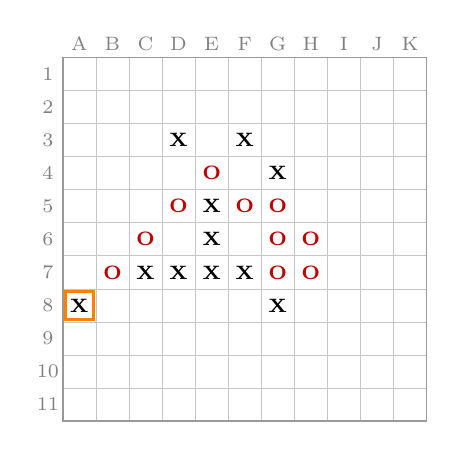
\begin{tikzpicture}[x=.42cm, y=.42cm]
\draw[gray!45, line width=.25pt] (0,0) -- (11,0);
\draw[gray!45, line width=.25pt] (0,0) -- (0,-11);
\draw[gray!45, line width=.25pt] (0,-1) -- (11,-1);
\draw[gray!45, line width=.25pt] (1,0) -- (1,-11);
\draw[gray!45, line width=.25pt] (0,-2) -- (11,-2);
\draw[gray!45, line width=.25pt] (2,0) -- (2,-11);
\draw[gray!45, line width=.25pt] (0,-3) -- (11,-3);
\draw[gray!45, line width=.25pt] (3,0) -- (3,-11);
\draw[gray!45, line width=.25pt] (0,-4) -- (11,-4);
\draw[gray!45, line width=.25pt] (4,0) -- (4,-11);
\draw[gray!45, line width=.25pt] (0,-5) -- (11,-5);
\draw[gray!45, line width=.25pt] (5,0) -- (5,-11);
\draw[gray!45, line width=.25pt] (0,-6) -- (11,-6);
\draw[gray!45, line width=.25pt] (6,0) -- (6,-11);
\draw[gray!45, line width=.25pt] (0,-7) -- (11,-7);
\draw[gray!45, line width=.25pt] (7,0) -- (7,-11);
\draw[gray!45, line width=.25pt] (0,-8) -- (11,-8);
\draw[gray!45, line width=.25pt] (8,0) -- (8,-11);
\draw[gray!45, line width=.25pt] (0,-9) -- (11,-9);
\draw[gray!45, line width=.25pt] (9,0) -- (9,-11);
\draw[gray!45, line width=.25pt] (0,-10) -- (11,-10);
\draw[gray!45, line width=.25pt] (10,0) -- (10,-11);
\draw[gray!45, line width=.25pt] (0,-11) -- (11,-11);
\draw[gray!45, line width=.25pt] (11,0) -- (11,-11);
\draw[gray!80, line width=.5pt] (0,0) rectangle (11,-11);
\node[font=\scriptsize, text=gray] at (0.5,.42) {A};
\node[font=\scriptsize, text=gray] at (1.5,.42) {B};
\node[font=\scriptsize, text=gray] at (2.5,.42) {C};
\node[font=\scriptsize, text=gray] at (3.5,.42) {D};
\node[font=\scriptsize, text=gray] at (4.5,.42) {E};
\node[font=\scriptsize, text=gray] at (5.5,.42) {F};
\node[font=\scriptsize, text=gray] at (6.5,.42) {G};
\node[font=\scriptsize, text=gray] at (7.5,.42) {H};
\node[font=\scriptsize, text=gray] at (8.5,.42) {I};
\node[font=\scriptsize, text=gray] at (9.5,.42) {J};
\node[font=\scriptsize, text=gray] at (10.5,.42) {K};
\node[font=\scriptsize, text=gray] at (-.45,-0.5) {1};
\node[font=\scriptsize, text=gray] at (-.45,-1.5) {2};
\node[font=\scriptsize, text=gray] at (-.45,-2.5) {3};
\node[font=\scriptsize, text=gray] at (-.45,-3.5) {4};
\node[font=\scriptsize, text=gray] at (-.45,-4.5) {5};
\node[font=\scriptsize, text=gray] at (-.45,-5.5) {6};
\node[font=\scriptsize, text=gray] at (-.45,-6.5) {7};
\node[font=\scriptsize, text=gray] at (-.45,-7.5) {8};
\node[font=\scriptsize, text=gray] at (-.45,-8.5) {9};
\node[font=\scriptsize, text=gray] at (-.45,-9.5) {10};
\node[font=\scriptsize, text=gray] at (-.45,-10.5) {11};
\node[text=black, font=\bfseries\scriptsize] at (3.5,-2.5) {X};
\node[text=black, font=\bfseries\scriptsize] at (5.5,-2.5) {X};
\node[text=red!75!black, font=\bfseries\scriptsize] at (4.5,-3.5) {O};
\node[text=black, font=\bfseries\scriptsize] at (6.5,-3.5) {X};
\node[text=red!75!black, font=\bfseries\scriptsize] at (3.5,-4.5) {O};
\node[text=black, font=\bfseries\scriptsize] at (4.5,-4.5) {X};
\node[text=red!75!black, font=\bfseries\scriptsize] at (5.5,-4.5) {O};
\node[text=red!75!black, font=\bfseries\scriptsize] at (6.5,-4.5) {O};
\node[text=red!75!black, font=\bfseries\scriptsize] at (2.5,-5.5) {O};
\node[text=black, font=\bfseries\scriptsize] at (4.5,-5.5) {X};
\node[text=red!75!black, font=\bfseries\scriptsize] at (6.5,-5.5) {O};
\node[text=red!75!black, font=\bfseries\scriptsize] at (7.5,-5.5) {O};
\node[text=red!75!black, font=\bfseries\scriptsize] at (1.5,-6.5) {O};
\node[text=black, font=\bfseries\scriptsize] at (2.5,-6.5) {X};
\node[text=black, font=\bfseries\scriptsize] at (3.5,-6.5) {X};
\node[text=black, font=\bfseries\scriptsize] at (4.5,-6.5) {X};
\node[text=black, font=\bfseries\scriptsize] at (5.5,-6.5) {X};
\node[text=red!75!black, font=\bfseries\scriptsize] at (6.5,-6.5) {O};
\node[text=red!75!black, font=\bfseries\scriptsize] at (7.5,-6.5) {O};
\node[text=black, font=\bfseries\scriptsize] at (0.5,-7.5) {X};
\draw[orange, line width=1pt] (0.08,-7.08) rectangle ++(.84,-.84);
\node[text=black, font=\bfseries\scriptsize] at (6.5,-7.5) {X};
\end{tikzpicture}
\end{center}
\paragraph{Thế kết thúc}
\begin{center}
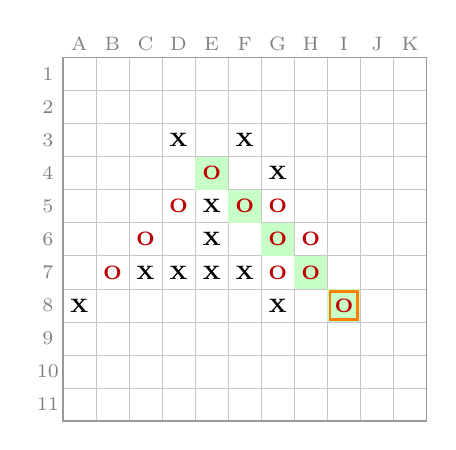
\begin{tikzpicture}[x=.42cm, y=.42cm]
\draw[gray!45, line width=.25pt] (0,0) -- (11,0);
\draw[gray!45, line width=.25pt] (0,0) -- (0,-11);
\draw[gray!45, line width=.25pt] (0,-1) -- (11,-1);
\draw[gray!45, line width=.25pt] (1,0) -- (1,-11);
\draw[gray!45, line width=.25pt] (0,-2) -- (11,-2);
\draw[gray!45, line width=.25pt] (2,0) -- (2,-11);
\draw[gray!45, line width=.25pt] (0,-3) -- (11,-3);
\draw[gray!45, line width=.25pt] (3,0) -- (3,-11);
\draw[gray!45, line width=.25pt] (0,-4) -- (11,-4);
\draw[gray!45, line width=.25pt] (4,0) -- (4,-11);
\draw[gray!45, line width=.25pt] (0,-5) -- (11,-5);
\draw[gray!45, line width=.25pt] (5,0) -- (5,-11);
\draw[gray!45, line width=.25pt] (0,-6) -- (11,-6);
\draw[gray!45, line width=.25pt] (6,0) -- (6,-11);
\draw[gray!45, line width=.25pt] (0,-7) -- (11,-7);
\draw[gray!45, line width=.25pt] (7,0) -- (7,-11);
\draw[gray!45, line width=.25pt] (0,-8) -- (11,-8);
\draw[gray!45, line width=.25pt] (8,0) -- (8,-11);
\draw[gray!45, line width=.25pt] (0,-9) -- (11,-9);
\draw[gray!45, line width=.25pt] (9,0) -- (9,-11);
\draw[gray!45, line width=.25pt] (0,-10) -- (11,-10);
\draw[gray!45, line width=.25pt] (10,0) -- (10,-11);
\draw[gray!45, line width=.25pt] (0,-11) -- (11,-11);
\draw[gray!45, line width=.25pt] (11,0) -- (11,-11);
\draw[gray!80, line width=.5pt] (0,0) rectangle (11,-11);
\node[font=\scriptsize, text=gray] at (0.5,.42) {A};
\node[font=\scriptsize, text=gray] at (1.5,.42) {B};
\node[font=\scriptsize, text=gray] at (2.5,.42) {C};
\node[font=\scriptsize, text=gray] at (3.5,.42) {D};
\node[font=\scriptsize, text=gray] at (4.5,.42) {E};
\node[font=\scriptsize, text=gray] at (5.5,.42) {F};
\node[font=\scriptsize, text=gray] at (6.5,.42) {G};
\node[font=\scriptsize, text=gray] at (7.5,.42) {H};
\node[font=\scriptsize, text=gray] at (8.5,.42) {I};
\node[font=\scriptsize, text=gray] at (9.5,.42) {J};
\node[font=\scriptsize, text=gray] at (10.5,.42) {K};
\node[font=\scriptsize, text=gray] at (-.45,-0.5) {1};
\node[font=\scriptsize, text=gray] at (-.45,-1.5) {2};
\node[font=\scriptsize, text=gray] at (-.45,-2.5) {3};
\node[font=\scriptsize, text=gray] at (-.45,-3.5) {4};
\node[font=\scriptsize, text=gray] at (-.45,-4.5) {5};
\node[font=\scriptsize, text=gray] at (-.45,-5.5) {6};
\node[font=\scriptsize, text=gray] at (-.45,-6.5) {7};
\node[font=\scriptsize, text=gray] at (-.45,-7.5) {8};
\node[font=\scriptsize, text=gray] at (-.45,-8.5) {9};
\node[font=\scriptsize, text=gray] at (-.45,-9.5) {10};
\node[font=\scriptsize, text=gray] at (-.45,-10.5) {11};
\node[text=black, font=\bfseries\scriptsize] at (3.5,-2.5) {X};
\node[text=black, font=\bfseries\scriptsize] at (5.5,-2.5) {X};
\fill[green!22] (4,-3) rectangle ++(1,-1);
\node[text=red!75!black, font=\bfseries\scriptsize] at (4.5,-3.5) {O};
\node[text=black, font=\bfseries\scriptsize] at (6.5,-3.5) {X};
\node[text=red!75!black, font=\bfseries\scriptsize] at (3.5,-4.5) {O};
\node[text=black, font=\bfseries\scriptsize] at (4.5,-4.5) {X};
\fill[green!22] (5,-4) rectangle ++(1,-1);
\node[text=red!75!black, font=\bfseries\scriptsize] at (5.5,-4.5) {O};
\node[text=red!75!black, font=\bfseries\scriptsize] at (6.5,-4.5) {O};
\node[text=red!75!black, font=\bfseries\scriptsize] at (2.5,-5.5) {O};
\node[text=black, font=\bfseries\scriptsize] at (4.5,-5.5) {X};
\fill[green!22] (6,-5) rectangle ++(1,-1);
\node[text=red!75!black, font=\bfseries\scriptsize] at (6.5,-5.5) {O};
\node[text=red!75!black, font=\bfseries\scriptsize] at (7.5,-5.5) {O};
\node[text=red!75!black, font=\bfseries\scriptsize] at (1.5,-6.5) {O};
\node[text=black, font=\bfseries\scriptsize] at (2.5,-6.5) {X};
\node[text=black, font=\bfseries\scriptsize] at (3.5,-6.5) {X};
\node[text=black, font=\bfseries\scriptsize] at (4.5,-6.5) {X};
\node[text=black, font=\bfseries\scriptsize] at (5.5,-6.5) {X};
\node[text=red!75!black, font=\bfseries\scriptsize] at (6.5,-6.5) {O};
\fill[green!22] (7,-6) rectangle ++(1,-1);
\node[text=red!75!black, font=\bfseries\scriptsize] at (7.5,-6.5) {O};
\node[text=black, font=\bfseries\scriptsize] at (0.5,-7.5) {X};
\node[text=black, font=\bfseries\scriptsize] at (6.5,-7.5) {X};
\fill[green!22] (8,-7) rectangle ++(1,-1);
\node[text=red!75!black, font=\bfseries\scriptsize] at (8.5,-7.5) {O};
\draw[orange, line width=1pt] (8.08,-7.08) rectangle ++(.84,-.84);
\end{tikzpicture}
\end{center}
\paragraph{Cơ chế kết thúc} Trước nước áp chót, bên thắng đã có 2 ô thắng ngay (A8, I8); đối thủ chỉ chặn được một ô, nên nước I8 hoàn thành dãy năm quân.
\paragraph{Nhận xét} L5 cầm O thắng L2 trong 22 nước, nhưng bỏ lỡ một nước thắng ngay ở nước 20. O vẫn thắng bằng đường chéo E4–I8 ở nước 22. Ván này cho thấy một lần bỏ lỡ thắng ngay không luôn dẫn đến thua, đặc biệt khi đối thủ không có đe doạ tức thì. Tuy nhiên, trong 402 cơ hội thắng ngay, L5 bỏ 54 lần; tỷ lệ này đủ để giải thích một phần khoảng cách giữa L5 và L6.
\paragraph{Diễn biến} {\footnotesize 1.E7 2.G5 3.F7 4.G7 5.D7 6.G6 7.G4 8.H6 9.C7 10.B7 11.E6 12.F5 13.G8 14.D5 15.E5 16.E4 17.D3 18.C6 19.F3 20.H7 21.A8 22.I8\par}

\subsection{RR8 · L6 thắng L3 · ván 900}
Khai cuộc gồm 3 nước: G6 → G5 → H5. X: \texttt{L3-AlphaBeta}, O: \texttt{L6-PolicyRL}. Kết quả: O thắng sau 34 nước.
\begin{center}\small
\begin{tabular}{@{}rccll@{}}
\toprule
Ply & Màu & Nước & Nhận xét & Ô liên quan \\
\midrule
14 & O & K6 & Chặn bắt buộc & K6 \\
17 & X & C9 & Chặn bắt buộc & C9 \\
27 & X & G11 & Chặn bắt buộc & G11 \\
29 & X & I11 & Chặn bắt buộc & I11 \\
31 & X & E11 & Chặn bắt buộc & E11 \\
34 & O & I10 & Thắng ngay & — \\
\bottomrule
\end{tabular}
\end{center}
\paragraph{Thế cờ trước nước quyết định (sau nước 33)}
\begin{center}
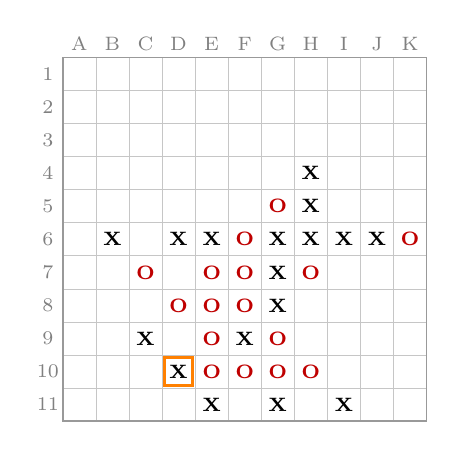
\begin{tikzpicture}[x=.42cm, y=.42cm]
\draw[gray!45, line width=.25pt] (0,0) -- (11,0);
\draw[gray!45, line width=.25pt] (0,0) -- (0,-11);
\draw[gray!45, line width=.25pt] (0,-1) -- (11,-1);
\draw[gray!45, line width=.25pt] (1,0) -- (1,-11);
\draw[gray!45, line width=.25pt] (0,-2) -- (11,-2);
\draw[gray!45, line width=.25pt] (2,0) -- (2,-11);
\draw[gray!45, line width=.25pt] (0,-3) -- (11,-3);
\draw[gray!45, line width=.25pt] (3,0) -- (3,-11);
\draw[gray!45, line width=.25pt] (0,-4) -- (11,-4);
\draw[gray!45, line width=.25pt] (4,0) -- (4,-11);
\draw[gray!45, line width=.25pt] (0,-5) -- (11,-5);
\draw[gray!45, line width=.25pt] (5,0) -- (5,-11);
\draw[gray!45, line width=.25pt] (0,-6) -- (11,-6);
\draw[gray!45, line width=.25pt] (6,0) -- (6,-11);
\draw[gray!45, line width=.25pt] (0,-7) -- (11,-7);
\draw[gray!45, line width=.25pt] (7,0) -- (7,-11);
\draw[gray!45, line width=.25pt] (0,-8) -- (11,-8);
\draw[gray!45, line width=.25pt] (8,0) -- (8,-11);
\draw[gray!45, line width=.25pt] (0,-9) -- (11,-9);
\draw[gray!45, line width=.25pt] (9,0) -- (9,-11);
\draw[gray!45, line width=.25pt] (0,-10) -- (11,-10);
\draw[gray!45, line width=.25pt] (10,0) -- (10,-11);
\draw[gray!45, line width=.25pt] (0,-11) -- (11,-11);
\draw[gray!45, line width=.25pt] (11,0) -- (11,-11);
\draw[gray!80, line width=.5pt] (0,0) rectangle (11,-11);
\node[font=\scriptsize, text=gray] at (0.5,.42) {A};
\node[font=\scriptsize, text=gray] at (1.5,.42) {B};
\node[font=\scriptsize, text=gray] at (2.5,.42) {C};
\node[font=\scriptsize, text=gray] at (3.5,.42) {D};
\node[font=\scriptsize, text=gray] at (4.5,.42) {E};
\node[font=\scriptsize, text=gray] at (5.5,.42) {F};
\node[font=\scriptsize, text=gray] at (6.5,.42) {G};
\node[font=\scriptsize, text=gray] at (7.5,.42) {H};
\node[font=\scriptsize, text=gray] at (8.5,.42) {I};
\node[font=\scriptsize, text=gray] at (9.5,.42) {J};
\node[font=\scriptsize, text=gray] at (10.5,.42) {K};
\node[font=\scriptsize, text=gray] at (-.45,-0.5) {1};
\node[font=\scriptsize, text=gray] at (-.45,-1.5) {2};
\node[font=\scriptsize, text=gray] at (-.45,-2.5) {3};
\node[font=\scriptsize, text=gray] at (-.45,-3.5) {4};
\node[font=\scriptsize, text=gray] at (-.45,-4.5) {5};
\node[font=\scriptsize, text=gray] at (-.45,-5.5) {6};
\node[font=\scriptsize, text=gray] at (-.45,-6.5) {7};
\node[font=\scriptsize, text=gray] at (-.45,-7.5) {8};
\node[font=\scriptsize, text=gray] at (-.45,-8.5) {9};
\node[font=\scriptsize, text=gray] at (-.45,-9.5) {10};
\node[font=\scriptsize, text=gray] at (-.45,-10.5) {11};
\node[text=black, font=\bfseries\scriptsize] at (7.5,-3.5) {X};
\node[text=red!75!black, font=\bfseries\scriptsize] at (6.5,-4.5) {O};
\node[text=black, font=\bfseries\scriptsize] at (7.5,-4.5) {X};
\node[text=black, font=\bfseries\scriptsize] at (1.5,-5.5) {X};
\node[text=black, font=\bfseries\scriptsize] at (3.5,-5.5) {X};
\node[text=black, font=\bfseries\scriptsize] at (4.5,-5.5) {X};
\node[text=red!75!black, font=\bfseries\scriptsize] at (5.5,-5.5) {O};
\node[text=black, font=\bfseries\scriptsize] at (6.5,-5.5) {X};
\node[text=black, font=\bfseries\scriptsize] at (7.5,-5.5) {X};
\node[text=black, font=\bfseries\scriptsize] at (8.5,-5.5) {X};
\node[text=black, font=\bfseries\scriptsize] at (9.5,-5.5) {X};
\node[text=red!75!black, font=\bfseries\scriptsize] at (10.5,-5.5) {O};
\node[text=red!75!black, font=\bfseries\scriptsize] at (2.5,-6.5) {O};
\node[text=red!75!black, font=\bfseries\scriptsize] at (4.5,-6.5) {O};
\node[text=red!75!black, font=\bfseries\scriptsize] at (5.5,-6.5) {O};
\node[text=black, font=\bfseries\scriptsize] at (6.5,-6.5) {X};
\node[text=red!75!black, font=\bfseries\scriptsize] at (7.5,-6.5) {O};
\node[text=red!75!black, font=\bfseries\scriptsize] at (3.5,-7.5) {O};
\node[text=red!75!black, font=\bfseries\scriptsize] at (4.5,-7.5) {O};
\node[text=red!75!black, font=\bfseries\scriptsize] at (5.5,-7.5) {O};
\node[text=black, font=\bfseries\scriptsize] at (6.5,-7.5) {X};
\node[text=black, font=\bfseries\scriptsize] at (2.5,-8.5) {X};
\node[text=red!75!black, font=\bfseries\scriptsize] at (4.5,-8.5) {O};
\node[text=black, font=\bfseries\scriptsize] at (5.5,-8.5) {X};
\node[text=red!75!black, font=\bfseries\scriptsize] at (6.5,-8.5) {O};
\node[text=black, font=\bfseries\scriptsize] at (3.5,-9.5) {X};
\draw[orange, line width=1pt] (3.08,-9.08) rectangle ++(.84,-.84);
\node[text=red!75!black, font=\bfseries\scriptsize] at (4.5,-9.5) {O};
\node[text=red!75!black, font=\bfseries\scriptsize] at (5.5,-9.5) {O};
\node[text=red!75!black, font=\bfseries\scriptsize] at (6.5,-9.5) {O};
\node[text=red!75!black, font=\bfseries\scriptsize] at (7.5,-9.5) {O};
\node[text=black, font=\bfseries\scriptsize] at (4.5,-10.5) {X};
\node[text=black, font=\bfseries\scriptsize] at (6.5,-10.5) {X};
\node[text=black, font=\bfseries\scriptsize] at (8.5,-10.5) {X};
\end{tikzpicture}
\end{center}
\paragraph{Thế kết thúc}
\begin{center}
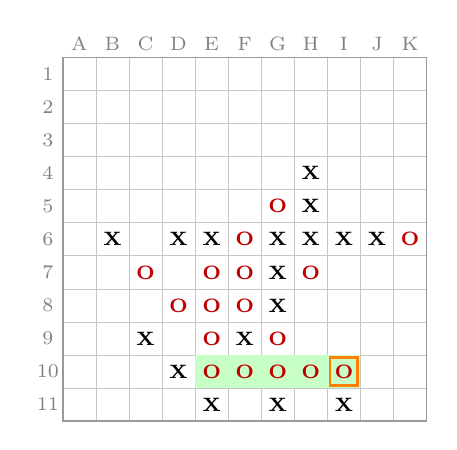
\begin{tikzpicture}[x=.42cm, y=.42cm]
\draw[gray!45, line width=.25pt] (0,0) -- (11,0);
\draw[gray!45, line width=.25pt] (0,0) -- (0,-11);
\draw[gray!45, line width=.25pt] (0,-1) -- (11,-1);
\draw[gray!45, line width=.25pt] (1,0) -- (1,-11);
\draw[gray!45, line width=.25pt] (0,-2) -- (11,-2);
\draw[gray!45, line width=.25pt] (2,0) -- (2,-11);
\draw[gray!45, line width=.25pt] (0,-3) -- (11,-3);
\draw[gray!45, line width=.25pt] (3,0) -- (3,-11);
\draw[gray!45, line width=.25pt] (0,-4) -- (11,-4);
\draw[gray!45, line width=.25pt] (4,0) -- (4,-11);
\draw[gray!45, line width=.25pt] (0,-5) -- (11,-5);
\draw[gray!45, line width=.25pt] (5,0) -- (5,-11);
\draw[gray!45, line width=.25pt] (0,-6) -- (11,-6);
\draw[gray!45, line width=.25pt] (6,0) -- (6,-11);
\draw[gray!45, line width=.25pt] (0,-7) -- (11,-7);
\draw[gray!45, line width=.25pt] (7,0) -- (7,-11);
\draw[gray!45, line width=.25pt] (0,-8) -- (11,-8);
\draw[gray!45, line width=.25pt] (8,0) -- (8,-11);
\draw[gray!45, line width=.25pt] (0,-9) -- (11,-9);
\draw[gray!45, line width=.25pt] (9,0) -- (9,-11);
\draw[gray!45, line width=.25pt] (0,-10) -- (11,-10);
\draw[gray!45, line width=.25pt] (10,0) -- (10,-11);
\draw[gray!45, line width=.25pt] (0,-11) -- (11,-11);
\draw[gray!45, line width=.25pt] (11,0) -- (11,-11);
\draw[gray!80, line width=.5pt] (0,0) rectangle (11,-11);
\node[font=\scriptsize, text=gray] at (0.5,.42) {A};
\node[font=\scriptsize, text=gray] at (1.5,.42) {B};
\node[font=\scriptsize, text=gray] at (2.5,.42) {C};
\node[font=\scriptsize, text=gray] at (3.5,.42) {D};
\node[font=\scriptsize, text=gray] at (4.5,.42) {E};
\node[font=\scriptsize, text=gray] at (5.5,.42) {F};
\node[font=\scriptsize, text=gray] at (6.5,.42) {G};
\node[font=\scriptsize, text=gray] at (7.5,.42) {H};
\node[font=\scriptsize, text=gray] at (8.5,.42) {I};
\node[font=\scriptsize, text=gray] at (9.5,.42) {J};
\node[font=\scriptsize, text=gray] at (10.5,.42) {K};
\node[font=\scriptsize, text=gray] at (-.45,-0.5) {1};
\node[font=\scriptsize, text=gray] at (-.45,-1.5) {2};
\node[font=\scriptsize, text=gray] at (-.45,-2.5) {3};
\node[font=\scriptsize, text=gray] at (-.45,-3.5) {4};
\node[font=\scriptsize, text=gray] at (-.45,-4.5) {5};
\node[font=\scriptsize, text=gray] at (-.45,-5.5) {6};
\node[font=\scriptsize, text=gray] at (-.45,-6.5) {7};
\node[font=\scriptsize, text=gray] at (-.45,-7.5) {8};
\node[font=\scriptsize, text=gray] at (-.45,-8.5) {9};
\node[font=\scriptsize, text=gray] at (-.45,-9.5) {10};
\node[font=\scriptsize, text=gray] at (-.45,-10.5) {11};
\node[text=black, font=\bfseries\scriptsize] at (7.5,-3.5) {X};
\node[text=red!75!black, font=\bfseries\scriptsize] at (6.5,-4.5) {O};
\node[text=black, font=\bfseries\scriptsize] at (7.5,-4.5) {X};
\node[text=black, font=\bfseries\scriptsize] at (1.5,-5.5) {X};
\node[text=black, font=\bfseries\scriptsize] at (3.5,-5.5) {X};
\node[text=black, font=\bfseries\scriptsize] at (4.5,-5.5) {X};
\node[text=red!75!black, font=\bfseries\scriptsize] at (5.5,-5.5) {O};
\node[text=black, font=\bfseries\scriptsize] at (6.5,-5.5) {X};
\node[text=black, font=\bfseries\scriptsize] at (7.5,-5.5) {X};
\node[text=black, font=\bfseries\scriptsize] at (8.5,-5.5) {X};
\node[text=black, font=\bfseries\scriptsize] at (9.5,-5.5) {X};
\node[text=red!75!black, font=\bfseries\scriptsize] at (10.5,-5.5) {O};
\node[text=red!75!black, font=\bfseries\scriptsize] at (2.5,-6.5) {O};
\node[text=red!75!black, font=\bfseries\scriptsize] at (4.5,-6.5) {O};
\node[text=red!75!black, font=\bfseries\scriptsize] at (5.5,-6.5) {O};
\node[text=black, font=\bfseries\scriptsize] at (6.5,-6.5) {X};
\node[text=red!75!black, font=\bfseries\scriptsize] at (7.5,-6.5) {O};
\node[text=red!75!black, font=\bfseries\scriptsize] at (3.5,-7.5) {O};
\node[text=red!75!black, font=\bfseries\scriptsize] at (4.5,-7.5) {O};
\node[text=red!75!black, font=\bfseries\scriptsize] at (5.5,-7.5) {O};
\node[text=black, font=\bfseries\scriptsize] at (6.5,-7.5) {X};
\node[text=black, font=\bfseries\scriptsize] at (2.5,-8.5) {X};
\node[text=red!75!black, font=\bfseries\scriptsize] at (4.5,-8.5) {O};
\node[text=black, font=\bfseries\scriptsize] at (5.5,-8.5) {X};
\node[text=red!75!black, font=\bfseries\scriptsize] at (6.5,-8.5) {O};
\node[text=black, font=\bfseries\scriptsize] at (3.5,-9.5) {X};
\fill[green!22] (4,-9) rectangle ++(1,-1);
\node[text=red!75!black, font=\bfseries\scriptsize] at (4.5,-9.5) {O};
\fill[green!22] (5,-9) rectangle ++(1,-1);
\node[text=red!75!black, font=\bfseries\scriptsize] at (5.5,-9.5) {O};
\fill[green!22] (6,-9) rectangle ++(1,-1);
\node[text=red!75!black, font=\bfseries\scriptsize] at (6.5,-9.5) {O};
\fill[green!22] (7,-9) rectangle ++(1,-1);
\node[text=red!75!black, font=\bfseries\scriptsize] at (7.5,-9.5) {O};
\fill[green!22] (8,-9) rectangle ++(1,-1);
\node[text=red!75!black, font=\bfseries\scriptsize] at (8.5,-9.5) {O};
\draw[orange, line width=1pt] (8.08,-9.08) rectangle ++(.84,-.84);
\node[text=black, font=\bfseries\scriptsize] at (4.5,-10.5) {X};
\node[text=black, font=\bfseries\scriptsize] at (6.5,-10.5) {X};
\node[text=black, font=\bfseries\scriptsize] at (8.5,-10.5) {X};
\end{tikzpicture}
\end{center}
\paragraph{Cơ chế kết thúc} Trước nước áp chót, bên thắng đã có 2 ô thắng ngay (D10, I10); đối thủ chỉ chặn được một ô, nên nước I10 hoàn thành dãy năm quân.
\paragraph{Nhận xét} L6 cầm O thắng L3 trong 34 nước bằng hàng ngang E10–I10. Không có lỗi bỏ chặn hay bỏ thắng ngay trong ván; khác biệt đến từ tích luỹ đe doạ và chọn cánh. Đây là ví dụ vì sao L6 (61,9\%) nhỉnh hơn L3 (58,3\%) dù khoảng tin cậy chồng lấn: RL học được một số mẫu tấn công mà Alpha-Beta độ sâu 4 không thấy.
\paragraph{Diễn biến} {\footnotesize 1.G6 2.G5 3.H5 4.F7 5.H6 6.F6 7.H4 8.H7 9.I6 10.E7 11.G7 12.F8 13.J6 14.K6 15.F9 16.D8 17.C9 18.E8 19.G8 20.G9 21.D6 22.E9 23.E6 24.C7 25.B6 26.F10 27.G11 28.H10 29.I11 30.E10 31.E11 32.G10 33.D10 34.I10\par}

\subsection{RR8 · L7 thắng L8 · ván 2401}
Khai cuộc gồm 4 nước: H8 → D6 → G5 → H6. X: \texttt{L7-PUCT}, O: \texttt{L8-AlphaZero}. Kết quả: X thắng sau 21 nước.
\begin{center}\small
\begin{tabular}{@{}rccll@{}}
\toprule
Ply & Màu & Nước & Nhận xét & Ô liên quan \\
\midrule
16 & O & G3 & Chặn bắt buộc & G3 \\
18 & O & E7 & Chặn bắt buộc & E7 \\
20 & O & H3 & Đã ở thế buộc thua & — \\
21 & X & C8 & Thắng ngay & — \\
\bottomrule
\end{tabular}
\end{center}
\paragraph{Thế cờ trước nước quyết định (sau nước 20)}
\begin{center}
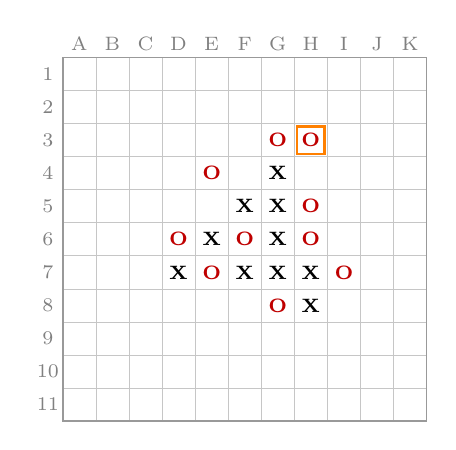
\begin{tikzpicture}[x=.42cm, y=.42cm]
\draw[gray!45, line width=.25pt] (0,0) -- (11,0);
\draw[gray!45, line width=.25pt] (0,0) -- (0,-11);
\draw[gray!45, line width=.25pt] (0,-1) -- (11,-1);
\draw[gray!45, line width=.25pt] (1,0) -- (1,-11);
\draw[gray!45, line width=.25pt] (0,-2) -- (11,-2);
\draw[gray!45, line width=.25pt] (2,0) -- (2,-11);
\draw[gray!45, line width=.25pt] (0,-3) -- (11,-3);
\draw[gray!45, line width=.25pt] (3,0) -- (3,-11);
\draw[gray!45, line width=.25pt] (0,-4) -- (11,-4);
\draw[gray!45, line width=.25pt] (4,0) -- (4,-11);
\draw[gray!45, line width=.25pt] (0,-5) -- (11,-5);
\draw[gray!45, line width=.25pt] (5,0) -- (5,-11);
\draw[gray!45, line width=.25pt] (0,-6) -- (11,-6);
\draw[gray!45, line width=.25pt] (6,0) -- (6,-11);
\draw[gray!45, line width=.25pt] (0,-7) -- (11,-7);
\draw[gray!45, line width=.25pt] (7,0) -- (7,-11);
\draw[gray!45, line width=.25pt] (0,-8) -- (11,-8);
\draw[gray!45, line width=.25pt] (8,0) -- (8,-11);
\draw[gray!45, line width=.25pt] (0,-9) -- (11,-9);
\draw[gray!45, line width=.25pt] (9,0) -- (9,-11);
\draw[gray!45, line width=.25pt] (0,-10) -- (11,-10);
\draw[gray!45, line width=.25pt] (10,0) -- (10,-11);
\draw[gray!45, line width=.25pt] (0,-11) -- (11,-11);
\draw[gray!45, line width=.25pt] (11,0) -- (11,-11);
\draw[gray!80, line width=.5pt] (0,0) rectangle (11,-11);
\node[font=\scriptsize, text=gray] at (0.5,.42) {A};
\node[font=\scriptsize, text=gray] at (1.5,.42) {B};
\node[font=\scriptsize, text=gray] at (2.5,.42) {C};
\node[font=\scriptsize, text=gray] at (3.5,.42) {D};
\node[font=\scriptsize, text=gray] at (4.5,.42) {E};
\node[font=\scriptsize, text=gray] at (5.5,.42) {F};
\node[font=\scriptsize, text=gray] at (6.5,.42) {G};
\node[font=\scriptsize, text=gray] at (7.5,.42) {H};
\node[font=\scriptsize, text=gray] at (8.5,.42) {I};
\node[font=\scriptsize, text=gray] at (9.5,.42) {J};
\node[font=\scriptsize, text=gray] at (10.5,.42) {K};
\node[font=\scriptsize, text=gray] at (-.45,-0.5) {1};
\node[font=\scriptsize, text=gray] at (-.45,-1.5) {2};
\node[font=\scriptsize, text=gray] at (-.45,-2.5) {3};
\node[font=\scriptsize, text=gray] at (-.45,-3.5) {4};
\node[font=\scriptsize, text=gray] at (-.45,-4.5) {5};
\node[font=\scriptsize, text=gray] at (-.45,-5.5) {6};
\node[font=\scriptsize, text=gray] at (-.45,-6.5) {7};
\node[font=\scriptsize, text=gray] at (-.45,-7.5) {8};
\node[font=\scriptsize, text=gray] at (-.45,-8.5) {9};
\node[font=\scriptsize, text=gray] at (-.45,-9.5) {10};
\node[font=\scriptsize, text=gray] at (-.45,-10.5) {11};
\node[text=red!75!black, font=\bfseries\scriptsize] at (6.5,-2.5) {O};
\node[text=red!75!black, font=\bfseries\scriptsize] at (7.5,-2.5) {O};
\draw[orange, line width=1pt] (7.08,-2.08) rectangle ++(.84,-.84);
\node[text=red!75!black, font=\bfseries\scriptsize] at (4.5,-3.5) {O};
\node[text=black, font=\bfseries\scriptsize] at (6.5,-3.5) {X};
\node[text=black, font=\bfseries\scriptsize] at (5.5,-4.5) {X};
\node[text=black, font=\bfseries\scriptsize] at (6.5,-4.5) {X};
\node[text=red!75!black, font=\bfseries\scriptsize] at (7.5,-4.5) {O};
\node[text=red!75!black, font=\bfseries\scriptsize] at (3.5,-5.5) {O};
\node[text=black, font=\bfseries\scriptsize] at (4.5,-5.5) {X};
\node[text=red!75!black, font=\bfseries\scriptsize] at (5.5,-5.5) {O};
\node[text=black, font=\bfseries\scriptsize] at (6.5,-5.5) {X};
\node[text=red!75!black, font=\bfseries\scriptsize] at (7.5,-5.5) {O};
\node[text=black, font=\bfseries\scriptsize] at (3.5,-6.5) {X};
\node[text=red!75!black, font=\bfseries\scriptsize] at (4.5,-6.5) {O};
\node[text=black, font=\bfseries\scriptsize] at (5.5,-6.5) {X};
\node[text=black, font=\bfseries\scriptsize] at (6.5,-6.5) {X};
\node[text=black, font=\bfseries\scriptsize] at (7.5,-6.5) {X};
\node[text=red!75!black, font=\bfseries\scriptsize] at (8.5,-6.5) {O};
\node[text=red!75!black, font=\bfseries\scriptsize] at (6.5,-7.5) {O};
\node[text=black, font=\bfseries\scriptsize] at (7.5,-7.5) {X};
\end{tikzpicture}
\end{center}
\paragraph{Thế kết thúc}
\begin{center}
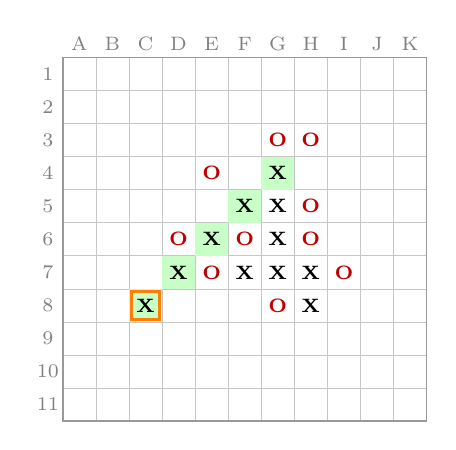
\begin{tikzpicture}[x=.42cm, y=.42cm]
\draw[gray!45, line width=.25pt] (0,0) -- (11,0);
\draw[gray!45, line width=.25pt] (0,0) -- (0,-11);
\draw[gray!45, line width=.25pt] (0,-1) -- (11,-1);
\draw[gray!45, line width=.25pt] (1,0) -- (1,-11);
\draw[gray!45, line width=.25pt] (0,-2) -- (11,-2);
\draw[gray!45, line width=.25pt] (2,0) -- (2,-11);
\draw[gray!45, line width=.25pt] (0,-3) -- (11,-3);
\draw[gray!45, line width=.25pt] (3,0) -- (3,-11);
\draw[gray!45, line width=.25pt] (0,-4) -- (11,-4);
\draw[gray!45, line width=.25pt] (4,0) -- (4,-11);
\draw[gray!45, line width=.25pt] (0,-5) -- (11,-5);
\draw[gray!45, line width=.25pt] (5,0) -- (5,-11);
\draw[gray!45, line width=.25pt] (0,-6) -- (11,-6);
\draw[gray!45, line width=.25pt] (6,0) -- (6,-11);
\draw[gray!45, line width=.25pt] (0,-7) -- (11,-7);
\draw[gray!45, line width=.25pt] (7,0) -- (7,-11);
\draw[gray!45, line width=.25pt] (0,-8) -- (11,-8);
\draw[gray!45, line width=.25pt] (8,0) -- (8,-11);
\draw[gray!45, line width=.25pt] (0,-9) -- (11,-9);
\draw[gray!45, line width=.25pt] (9,0) -- (9,-11);
\draw[gray!45, line width=.25pt] (0,-10) -- (11,-10);
\draw[gray!45, line width=.25pt] (10,0) -- (10,-11);
\draw[gray!45, line width=.25pt] (0,-11) -- (11,-11);
\draw[gray!45, line width=.25pt] (11,0) -- (11,-11);
\draw[gray!80, line width=.5pt] (0,0) rectangle (11,-11);
\node[font=\scriptsize, text=gray] at (0.5,.42) {A};
\node[font=\scriptsize, text=gray] at (1.5,.42) {B};
\node[font=\scriptsize, text=gray] at (2.5,.42) {C};
\node[font=\scriptsize, text=gray] at (3.5,.42) {D};
\node[font=\scriptsize, text=gray] at (4.5,.42) {E};
\node[font=\scriptsize, text=gray] at (5.5,.42) {F};
\node[font=\scriptsize, text=gray] at (6.5,.42) {G};
\node[font=\scriptsize, text=gray] at (7.5,.42) {H};
\node[font=\scriptsize, text=gray] at (8.5,.42) {I};
\node[font=\scriptsize, text=gray] at (9.5,.42) {J};
\node[font=\scriptsize, text=gray] at (10.5,.42) {K};
\node[font=\scriptsize, text=gray] at (-.45,-0.5) {1};
\node[font=\scriptsize, text=gray] at (-.45,-1.5) {2};
\node[font=\scriptsize, text=gray] at (-.45,-2.5) {3};
\node[font=\scriptsize, text=gray] at (-.45,-3.5) {4};
\node[font=\scriptsize, text=gray] at (-.45,-4.5) {5};
\node[font=\scriptsize, text=gray] at (-.45,-5.5) {6};
\node[font=\scriptsize, text=gray] at (-.45,-6.5) {7};
\node[font=\scriptsize, text=gray] at (-.45,-7.5) {8};
\node[font=\scriptsize, text=gray] at (-.45,-8.5) {9};
\node[font=\scriptsize, text=gray] at (-.45,-9.5) {10};
\node[font=\scriptsize, text=gray] at (-.45,-10.5) {11};
\node[text=red!75!black, font=\bfseries\scriptsize] at (6.5,-2.5) {O};
\node[text=red!75!black, font=\bfseries\scriptsize] at (7.5,-2.5) {O};
\node[text=red!75!black, font=\bfseries\scriptsize] at (4.5,-3.5) {O};
\fill[green!22] (6,-3) rectangle ++(1,-1);
\node[text=black, font=\bfseries\scriptsize] at (6.5,-3.5) {X};
\fill[green!22] (5,-4) rectangle ++(1,-1);
\node[text=black, font=\bfseries\scriptsize] at (5.5,-4.5) {X};
\node[text=black, font=\bfseries\scriptsize] at (6.5,-4.5) {X};
\node[text=red!75!black, font=\bfseries\scriptsize] at (7.5,-4.5) {O};
\node[text=red!75!black, font=\bfseries\scriptsize] at (3.5,-5.5) {O};
\fill[green!22] (4,-5) rectangle ++(1,-1);
\node[text=black, font=\bfseries\scriptsize] at (4.5,-5.5) {X};
\node[text=red!75!black, font=\bfseries\scriptsize] at (5.5,-5.5) {O};
\node[text=black, font=\bfseries\scriptsize] at (6.5,-5.5) {X};
\node[text=red!75!black, font=\bfseries\scriptsize] at (7.5,-5.5) {O};
\fill[green!22] (3,-6) rectangle ++(1,-1);
\node[text=black, font=\bfseries\scriptsize] at (3.5,-6.5) {X};
\node[text=red!75!black, font=\bfseries\scriptsize] at (4.5,-6.5) {O};
\node[text=black, font=\bfseries\scriptsize] at (5.5,-6.5) {X};
\node[text=black, font=\bfseries\scriptsize] at (6.5,-6.5) {X};
\node[text=black, font=\bfseries\scriptsize] at (7.5,-6.5) {X};
\node[text=red!75!black, font=\bfseries\scriptsize] at (8.5,-6.5) {O};
\fill[green!22] (2,-7) rectangle ++(1,-1);
\node[text=black, font=\bfseries\scriptsize] at (2.5,-7.5) {X};
\draw[orange, line width=1pt] (2.08,-7.08) rectangle ++(.84,-.84);
\node[text=red!75!black, font=\bfseries\scriptsize] at (6.5,-7.5) {O};
\node[text=black, font=\bfseries\scriptsize] at (7.5,-7.5) {X};
\end{tikzpicture}
\end{center}
\paragraph{Cơ chế kết thúc} Trước nước áp chót, bên thắng đã có 2 ô thắng ngay (H3, C8); đối thủ chỉ chặn được một ô, nên nước C8 hoàn thành dãy năm quân.
\paragraph{Nhận xét} L7 cầm X thắng L8 trong 21 nước bằng đường chéo G4–C8. Đây là một trong 34 ván L7 thắng L8 trên 100 ván cặp này; tỷ lệ 34\% là cao hơn nhiều so với các tác tử khác trước L8. Ván cho thấy L8 không bất khả chiến bại: khi L7 tạo được đe doạ chéo sớm, L8 cũng bị cuốn vào thế phòng thủ.
\paragraph{Diễn biến} {\footnotesize 1.H8 2.D6 3.G5 4.H6 5.G7 6.F6 7.G6 8.G8 9.F7 10.H5 11.H7 12.I7 13.F5 14.E4 15.G4 16.G3 17.D7 18.E7 19.E6 20.H3 21.C8\par}

\subsection{RR8 · L8 thắng L7 · ván 2402}
Khai cuộc gồm 2 nước: H7 → H8. X: \texttt{L7-PUCT}, O: \texttt{L8-AlphaZero}. Kết quả: O thắng sau 64 nước.
\begin{center}\small
\begin{tabular}{@{}rccll@{}}
\toprule
Ply & Màu & Nước & Nhận xét & Ô liên quan \\
\midrule
12 & O & K7 & Chặn bắt buộc & K7 \\
24 & O & K9 & Chặn bắt buộc & K9 \\
38 & O & I9 & Chặn bắt buộc & I9 \\
41 & X & F6 & Chặn bắt buộc & F6 \\
43 & X & F1 & Chặn bắt buộc & F1 \\
46 & O & C5 & Chặn bắt buộc & C5 \\
\bottomrule
\end{tabular}
\end{center}
\paragraph{Thế cờ trước nước quyết định (sau nước 45)}
\begin{center}
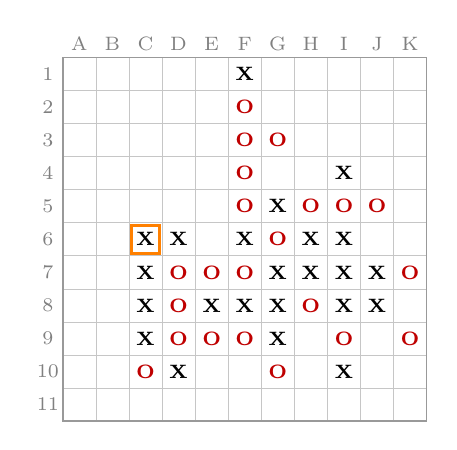
\begin{tikzpicture}[x=.42cm, y=.42cm]
\draw[gray!45, line width=.25pt] (0,0) -- (11,0);
\draw[gray!45, line width=.25pt] (0,0) -- (0,-11);
\draw[gray!45, line width=.25pt] (0,-1) -- (11,-1);
\draw[gray!45, line width=.25pt] (1,0) -- (1,-11);
\draw[gray!45, line width=.25pt] (0,-2) -- (11,-2);
\draw[gray!45, line width=.25pt] (2,0) -- (2,-11);
\draw[gray!45, line width=.25pt] (0,-3) -- (11,-3);
\draw[gray!45, line width=.25pt] (3,0) -- (3,-11);
\draw[gray!45, line width=.25pt] (0,-4) -- (11,-4);
\draw[gray!45, line width=.25pt] (4,0) -- (4,-11);
\draw[gray!45, line width=.25pt] (0,-5) -- (11,-5);
\draw[gray!45, line width=.25pt] (5,0) -- (5,-11);
\draw[gray!45, line width=.25pt] (0,-6) -- (11,-6);
\draw[gray!45, line width=.25pt] (6,0) -- (6,-11);
\draw[gray!45, line width=.25pt] (0,-7) -- (11,-7);
\draw[gray!45, line width=.25pt] (7,0) -- (7,-11);
\draw[gray!45, line width=.25pt] (0,-8) -- (11,-8);
\draw[gray!45, line width=.25pt] (8,0) -- (8,-11);
\draw[gray!45, line width=.25pt] (0,-9) -- (11,-9);
\draw[gray!45, line width=.25pt] (9,0) -- (9,-11);
\draw[gray!45, line width=.25pt] (0,-10) -- (11,-10);
\draw[gray!45, line width=.25pt] (10,0) -- (10,-11);
\draw[gray!45, line width=.25pt] (0,-11) -- (11,-11);
\draw[gray!45, line width=.25pt] (11,0) -- (11,-11);
\draw[gray!80, line width=.5pt] (0,0) rectangle (11,-11);
\node[font=\scriptsize, text=gray] at (0.5,.42) {A};
\node[font=\scriptsize, text=gray] at (1.5,.42) {B};
\node[font=\scriptsize, text=gray] at (2.5,.42) {C};
\node[font=\scriptsize, text=gray] at (3.5,.42) {D};
\node[font=\scriptsize, text=gray] at (4.5,.42) {E};
\node[font=\scriptsize, text=gray] at (5.5,.42) {F};
\node[font=\scriptsize, text=gray] at (6.5,.42) {G};
\node[font=\scriptsize, text=gray] at (7.5,.42) {H};
\node[font=\scriptsize, text=gray] at (8.5,.42) {I};
\node[font=\scriptsize, text=gray] at (9.5,.42) {J};
\node[font=\scriptsize, text=gray] at (10.5,.42) {K};
\node[font=\scriptsize, text=gray] at (-.45,-0.5) {1};
\node[font=\scriptsize, text=gray] at (-.45,-1.5) {2};
\node[font=\scriptsize, text=gray] at (-.45,-2.5) {3};
\node[font=\scriptsize, text=gray] at (-.45,-3.5) {4};
\node[font=\scriptsize, text=gray] at (-.45,-4.5) {5};
\node[font=\scriptsize, text=gray] at (-.45,-5.5) {6};
\node[font=\scriptsize, text=gray] at (-.45,-6.5) {7};
\node[font=\scriptsize, text=gray] at (-.45,-7.5) {8};
\node[font=\scriptsize, text=gray] at (-.45,-8.5) {9};
\node[font=\scriptsize, text=gray] at (-.45,-9.5) {10};
\node[font=\scriptsize, text=gray] at (-.45,-10.5) {11};
\node[text=black, font=\bfseries\scriptsize] at (5.5,-0.5) {X};
\node[text=red!75!black, font=\bfseries\scriptsize] at (5.5,-1.5) {O};
\node[text=red!75!black, font=\bfseries\scriptsize] at (5.5,-2.5) {O};
\node[text=red!75!black, font=\bfseries\scriptsize] at (6.5,-2.5) {O};
\node[text=red!75!black, font=\bfseries\scriptsize] at (5.5,-3.5) {O};
\node[text=black, font=\bfseries\scriptsize] at (8.5,-3.5) {X};
\node[text=red!75!black, font=\bfseries\scriptsize] at (5.5,-4.5) {O};
\node[text=black, font=\bfseries\scriptsize] at (6.5,-4.5) {X};
\node[text=red!75!black, font=\bfseries\scriptsize] at (7.5,-4.5) {O};
\node[text=red!75!black, font=\bfseries\scriptsize] at (8.5,-4.5) {O};
\node[text=red!75!black, font=\bfseries\scriptsize] at (9.5,-4.5) {O};
\node[text=black, font=\bfseries\scriptsize] at (2.5,-5.5) {X};
\draw[orange, line width=1pt] (2.08,-5.08) rectangle ++(.84,-.84);
\node[text=black, font=\bfseries\scriptsize] at (3.5,-5.5) {X};
\node[text=black, font=\bfseries\scriptsize] at (5.5,-5.5) {X};
\node[text=red!75!black, font=\bfseries\scriptsize] at (6.5,-5.5) {O};
\node[text=black, font=\bfseries\scriptsize] at (7.5,-5.5) {X};
\node[text=black, font=\bfseries\scriptsize] at (8.5,-5.5) {X};
\node[text=black, font=\bfseries\scriptsize] at (2.5,-6.5) {X};
\node[text=red!75!black, font=\bfseries\scriptsize] at (3.5,-6.5) {O};
\node[text=red!75!black, font=\bfseries\scriptsize] at (4.5,-6.5) {O};
\node[text=red!75!black, font=\bfseries\scriptsize] at (5.5,-6.5) {O};
\node[text=black, font=\bfseries\scriptsize] at (6.5,-6.5) {X};
\node[text=black, font=\bfseries\scriptsize] at (7.5,-6.5) {X};
\node[text=black, font=\bfseries\scriptsize] at (8.5,-6.5) {X};
\node[text=black, font=\bfseries\scriptsize] at (9.5,-6.5) {X};
\node[text=red!75!black, font=\bfseries\scriptsize] at (10.5,-6.5) {O};
\node[text=black, font=\bfseries\scriptsize] at (2.5,-7.5) {X};
\node[text=red!75!black, font=\bfseries\scriptsize] at (3.5,-7.5) {O};
\node[text=black, font=\bfseries\scriptsize] at (4.5,-7.5) {X};
\node[text=black, font=\bfseries\scriptsize] at (5.5,-7.5) {X};
\node[text=black, font=\bfseries\scriptsize] at (6.5,-7.5) {X};
\node[text=red!75!black, font=\bfseries\scriptsize] at (7.5,-7.5) {O};
\node[text=black, font=\bfseries\scriptsize] at (8.5,-7.5) {X};
\node[text=black, font=\bfseries\scriptsize] at (9.5,-7.5) {X};
\node[text=black, font=\bfseries\scriptsize] at (2.5,-8.5) {X};
\node[text=red!75!black, font=\bfseries\scriptsize] at (3.5,-8.5) {O};
\node[text=red!75!black, font=\bfseries\scriptsize] at (4.5,-8.5) {O};
\node[text=red!75!black, font=\bfseries\scriptsize] at (5.5,-8.5) {O};
\node[text=black, font=\bfseries\scriptsize] at (6.5,-8.5) {X};
\node[text=red!75!black, font=\bfseries\scriptsize] at (8.5,-8.5) {O};
\node[text=red!75!black, font=\bfseries\scriptsize] at (10.5,-8.5) {O};
\node[text=red!75!black, font=\bfseries\scriptsize] at (2.5,-9.5) {O};
\node[text=black, font=\bfseries\scriptsize] at (3.5,-9.5) {X};
\node[text=red!75!black, font=\bfseries\scriptsize] at (6.5,-9.5) {O};
\node[text=black, font=\bfseries\scriptsize] at (8.5,-9.5) {X};
\end{tikzpicture}
\end{center}
\paragraph{Thế kết thúc}
\begin{center}
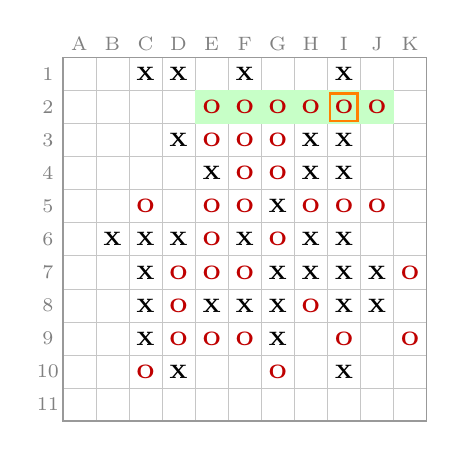
\begin{tikzpicture}[x=.42cm, y=.42cm]
\draw[gray!45, line width=.25pt] (0,0) -- (11,0);
\draw[gray!45, line width=.25pt] (0,0) -- (0,-11);
\draw[gray!45, line width=.25pt] (0,-1) -- (11,-1);
\draw[gray!45, line width=.25pt] (1,0) -- (1,-11);
\draw[gray!45, line width=.25pt] (0,-2) -- (11,-2);
\draw[gray!45, line width=.25pt] (2,0) -- (2,-11);
\draw[gray!45, line width=.25pt] (0,-3) -- (11,-3);
\draw[gray!45, line width=.25pt] (3,0) -- (3,-11);
\draw[gray!45, line width=.25pt] (0,-4) -- (11,-4);
\draw[gray!45, line width=.25pt] (4,0) -- (4,-11);
\draw[gray!45, line width=.25pt] (0,-5) -- (11,-5);
\draw[gray!45, line width=.25pt] (5,0) -- (5,-11);
\draw[gray!45, line width=.25pt] (0,-6) -- (11,-6);
\draw[gray!45, line width=.25pt] (6,0) -- (6,-11);
\draw[gray!45, line width=.25pt] (0,-7) -- (11,-7);
\draw[gray!45, line width=.25pt] (7,0) -- (7,-11);
\draw[gray!45, line width=.25pt] (0,-8) -- (11,-8);
\draw[gray!45, line width=.25pt] (8,0) -- (8,-11);
\draw[gray!45, line width=.25pt] (0,-9) -- (11,-9);
\draw[gray!45, line width=.25pt] (9,0) -- (9,-11);
\draw[gray!45, line width=.25pt] (0,-10) -- (11,-10);
\draw[gray!45, line width=.25pt] (10,0) -- (10,-11);
\draw[gray!45, line width=.25pt] (0,-11) -- (11,-11);
\draw[gray!45, line width=.25pt] (11,0) -- (11,-11);
\draw[gray!80, line width=.5pt] (0,0) rectangle (11,-11);
\node[font=\scriptsize, text=gray] at (0.5,.42) {A};
\node[font=\scriptsize, text=gray] at (1.5,.42) {B};
\node[font=\scriptsize, text=gray] at (2.5,.42) {C};
\node[font=\scriptsize, text=gray] at (3.5,.42) {D};
\node[font=\scriptsize, text=gray] at (4.5,.42) {E};
\node[font=\scriptsize, text=gray] at (5.5,.42) {F};
\node[font=\scriptsize, text=gray] at (6.5,.42) {G};
\node[font=\scriptsize, text=gray] at (7.5,.42) {H};
\node[font=\scriptsize, text=gray] at (8.5,.42) {I};
\node[font=\scriptsize, text=gray] at (9.5,.42) {J};
\node[font=\scriptsize, text=gray] at (10.5,.42) {K};
\node[font=\scriptsize, text=gray] at (-.45,-0.5) {1};
\node[font=\scriptsize, text=gray] at (-.45,-1.5) {2};
\node[font=\scriptsize, text=gray] at (-.45,-2.5) {3};
\node[font=\scriptsize, text=gray] at (-.45,-3.5) {4};
\node[font=\scriptsize, text=gray] at (-.45,-4.5) {5};
\node[font=\scriptsize, text=gray] at (-.45,-5.5) {6};
\node[font=\scriptsize, text=gray] at (-.45,-6.5) {7};
\node[font=\scriptsize, text=gray] at (-.45,-7.5) {8};
\node[font=\scriptsize, text=gray] at (-.45,-8.5) {9};
\node[font=\scriptsize, text=gray] at (-.45,-9.5) {10};
\node[font=\scriptsize, text=gray] at (-.45,-10.5) {11};
\node[text=black, font=\bfseries\scriptsize] at (2.5,-0.5) {X};
\node[text=black, font=\bfseries\scriptsize] at (3.5,-0.5) {X};
\node[text=black, font=\bfseries\scriptsize] at (5.5,-0.5) {X};
\node[text=black, font=\bfseries\scriptsize] at (8.5,-0.5) {X};
\fill[green!22] (4,-1) rectangle ++(1,-1);
\node[text=red!75!black, font=\bfseries\scriptsize] at (4.5,-1.5) {O};
\fill[green!22] (5,-1) rectangle ++(1,-1);
\node[text=red!75!black, font=\bfseries\scriptsize] at (5.5,-1.5) {O};
\fill[green!22] (6,-1) rectangle ++(1,-1);
\node[text=red!75!black, font=\bfseries\scriptsize] at (6.5,-1.5) {O};
\fill[green!22] (7,-1) rectangle ++(1,-1);
\node[text=red!75!black, font=\bfseries\scriptsize] at (7.5,-1.5) {O};
\fill[green!22] (8,-1) rectangle ++(1,-1);
\node[text=red!75!black, font=\bfseries\scriptsize] at (8.5,-1.5) {O};
\draw[orange, line width=1pt] (8.08,-1.08) rectangle ++(.84,-.84);
\fill[green!22] (9,-1) rectangle ++(1,-1);
\node[text=red!75!black, font=\bfseries\scriptsize] at (9.5,-1.5) {O};
\node[text=black, font=\bfseries\scriptsize] at (3.5,-2.5) {X};
\node[text=red!75!black, font=\bfseries\scriptsize] at (4.5,-2.5) {O};
\node[text=red!75!black, font=\bfseries\scriptsize] at (5.5,-2.5) {O};
\node[text=red!75!black, font=\bfseries\scriptsize] at (6.5,-2.5) {O};
\node[text=black, font=\bfseries\scriptsize] at (7.5,-2.5) {X};
\node[text=black, font=\bfseries\scriptsize] at (8.5,-2.5) {X};
\node[text=black, font=\bfseries\scriptsize] at (4.5,-3.5) {X};
\node[text=red!75!black, font=\bfseries\scriptsize] at (5.5,-3.5) {O};
\node[text=red!75!black, font=\bfseries\scriptsize] at (6.5,-3.5) {O};
\node[text=black, font=\bfseries\scriptsize] at (7.5,-3.5) {X};
\node[text=black, font=\bfseries\scriptsize] at (8.5,-3.5) {X};
\node[text=red!75!black, font=\bfseries\scriptsize] at (2.5,-4.5) {O};
\node[text=red!75!black, font=\bfseries\scriptsize] at (4.5,-4.5) {O};
\node[text=red!75!black, font=\bfseries\scriptsize] at (5.5,-4.5) {O};
\node[text=black, font=\bfseries\scriptsize] at (6.5,-4.5) {X};
\node[text=red!75!black, font=\bfseries\scriptsize] at (7.5,-4.5) {O};
\node[text=red!75!black, font=\bfseries\scriptsize] at (8.5,-4.5) {O};
\node[text=red!75!black, font=\bfseries\scriptsize] at (9.5,-4.5) {O};
\node[text=black, font=\bfseries\scriptsize] at (1.5,-5.5) {X};
\node[text=black, font=\bfseries\scriptsize] at (2.5,-5.5) {X};
\node[text=black, font=\bfseries\scriptsize] at (3.5,-5.5) {X};
\node[text=red!75!black, font=\bfseries\scriptsize] at (4.5,-5.5) {O};
\node[text=black, font=\bfseries\scriptsize] at (5.5,-5.5) {X};
\node[text=red!75!black, font=\bfseries\scriptsize] at (6.5,-5.5) {O};
\node[text=black, font=\bfseries\scriptsize] at (7.5,-5.5) {X};
\node[text=black, font=\bfseries\scriptsize] at (8.5,-5.5) {X};
\node[text=black, font=\bfseries\scriptsize] at (2.5,-6.5) {X};
\node[text=red!75!black, font=\bfseries\scriptsize] at (3.5,-6.5) {O};
\node[text=red!75!black, font=\bfseries\scriptsize] at (4.5,-6.5) {O};
\node[text=red!75!black, font=\bfseries\scriptsize] at (5.5,-6.5) {O};
\node[text=black, font=\bfseries\scriptsize] at (6.5,-6.5) {X};
\node[text=black, font=\bfseries\scriptsize] at (7.5,-6.5) {X};
\node[text=black, font=\bfseries\scriptsize] at (8.5,-6.5) {X};
\node[text=black, font=\bfseries\scriptsize] at (9.5,-6.5) {X};
\node[text=red!75!black, font=\bfseries\scriptsize] at (10.5,-6.5) {O};
\node[text=black, font=\bfseries\scriptsize] at (2.5,-7.5) {X};
\node[text=red!75!black, font=\bfseries\scriptsize] at (3.5,-7.5) {O};
\node[text=black, font=\bfseries\scriptsize] at (4.5,-7.5) {X};
\node[text=black, font=\bfseries\scriptsize] at (5.5,-7.5) {X};
\node[text=black, font=\bfseries\scriptsize] at (6.5,-7.5) {X};
\node[text=red!75!black, font=\bfseries\scriptsize] at (7.5,-7.5) {O};
\node[text=black, font=\bfseries\scriptsize] at (8.5,-7.5) {X};
\node[text=black, font=\bfseries\scriptsize] at (9.5,-7.5) {X};
\node[text=black, font=\bfseries\scriptsize] at (2.5,-8.5) {X};
\node[text=red!75!black, font=\bfseries\scriptsize] at (3.5,-8.5) {O};
\node[text=red!75!black, font=\bfseries\scriptsize] at (4.5,-8.5) {O};
\node[text=red!75!black, font=\bfseries\scriptsize] at (5.5,-8.5) {O};
\node[text=black, font=\bfseries\scriptsize] at (6.5,-8.5) {X};
\node[text=red!75!black, font=\bfseries\scriptsize] at (8.5,-8.5) {O};
\node[text=red!75!black, font=\bfseries\scriptsize] at (10.5,-8.5) {O};
\node[text=red!75!black, font=\bfseries\scriptsize] at (2.5,-9.5) {O};
\node[text=black, font=\bfseries\scriptsize] at (3.5,-9.5) {X};
\node[text=red!75!black, font=\bfseries\scriptsize] at (6.5,-9.5) {O};
\node[text=black, font=\bfseries\scriptsize] at (8.5,-9.5) {X};
\end{tikzpicture}
\end{center}
\paragraph{Cơ chế kết thúc} Trước nước áp chót, bên thắng đã có 2 ô thắng ngay (D2, I2); đối thủ chỉ chặn được một ô, nên nước I2 hoàn thành dãy năm quân.
\paragraph{Nhận xét} L8 cầm O thắng L7 sau 64 nước bằng hàng ngang E2–J2 (sáu quân). Ván dài, nhiều lần đổi cánh, kết thúc bằng một hàng ngang sát biên. Đây là ví dụ L8 không chỉ thắng nhanh ở trung tâm mà còn biết kéo dài và chuyển cánh khi cần. Trong cặp L7–L8, L8 thắng 66/100 ván, nhưng 34 ván thua cho thấy khoảng cách không tuyệt đối.
\paragraph{Diễn biến} {\footnotesize 1.H7 2.H8 3.G7 4.F7 5.G8 6.G6 7.I6 8.J5 9.I7 10.H5 11.J7 12.K7 13.I4 14.I5 15.G5 16.F9 17.H6 18.F4 19.F8 20.E9 21.E8 22.D9 23.J8 24.K9 25.G9 26.D8 27.I8 28.G10 29.C7 30.D7 31.D6 32.E7 33.C9 34.F5 35.C8 36.C10 37.I10 38.I9 39.D10 40.F3 41.F6 42.F2 43.F1 44.G3 45.C6 46.C5 47.H4 48.E3 49.I3 50.J2 51.B6 52.E6 53.D3 54.E5 55.E4 56.H2 57.I1 58.G4 59.H3 60.E2 61.D1 62.G2 63.C1 64.I2\par}

\subsection{RR8 · hoà L7–L8 · ván 2400}
Khai cuộc gồm 3 nước: G6 → G5 → H5. X: \texttt{L7-PUCT}, O: \texttt{L8-AlphaZero}. Kết quả: hoà sau 121 nước.
\begin{center}\small
\begin{tabular}{@{}rccll@{}}
\toprule
Ply & Màu & Nước & Nhận xét & Ô liên quan \\
\midrule
13 & X & F3 & Chặn bắt buộc & F3 \\
21 & X & B3 & Chặn bắt buộc & B3 \\
23 & X & J2 & Chặn bắt buộc & J2 \\
25 & X & I4 & Chặn bắt buộc & I4 \\
29 & X & E5 & Chặn bắt buộc & E5 \\
31 & X & D7 & Chặn bắt buộc & D7 \\
\bottomrule
\end{tabular}
\end{center}
\paragraph{Thế cờ trước nước quyết định (sau nước 30)}
\begin{center}
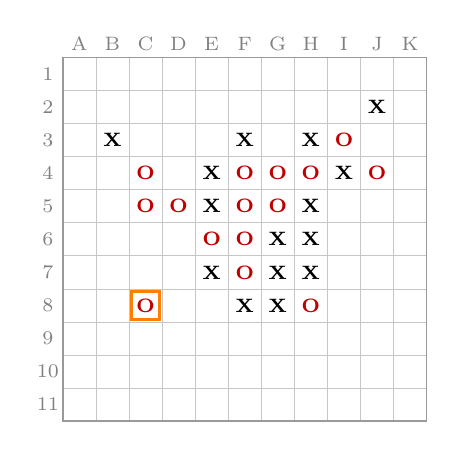
\begin{tikzpicture}[x=.42cm, y=.42cm]
\draw[gray!45, line width=.25pt] (0,0) -- (11,0);
\draw[gray!45, line width=.25pt] (0,0) -- (0,-11);
\draw[gray!45, line width=.25pt] (0,-1) -- (11,-1);
\draw[gray!45, line width=.25pt] (1,0) -- (1,-11);
\draw[gray!45, line width=.25pt] (0,-2) -- (11,-2);
\draw[gray!45, line width=.25pt] (2,0) -- (2,-11);
\draw[gray!45, line width=.25pt] (0,-3) -- (11,-3);
\draw[gray!45, line width=.25pt] (3,0) -- (3,-11);
\draw[gray!45, line width=.25pt] (0,-4) -- (11,-4);
\draw[gray!45, line width=.25pt] (4,0) -- (4,-11);
\draw[gray!45, line width=.25pt] (0,-5) -- (11,-5);
\draw[gray!45, line width=.25pt] (5,0) -- (5,-11);
\draw[gray!45, line width=.25pt] (0,-6) -- (11,-6);
\draw[gray!45, line width=.25pt] (6,0) -- (6,-11);
\draw[gray!45, line width=.25pt] (0,-7) -- (11,-7);
\draw[gray!45, line width=.25pt] (7,0) -- (7,-11);
\draw[gray!45, line width=.25pt] (0,-8) -- (11,-8);
\draw[gray!45, line width=.25pt] (8,0) -- (8,-11);
\draw[gray!45, line width=.25pt] (0,-9) -- (11,-9);
\draw[gray!45, line width=.25pt] (9,0) -- (9,-11);
\draw[gray!45, line width=.25pt] (0,-10) -- (11,-10);
\draw[gray!45, line width=.25pt] (10,0) -- (10,-11);
\draw[gray!45, line width=.25pt] (0,-11) -- (11,-11);
\draw[gray!45, line width=.25pt] (11,0) -- (11,-11);
\draw[gray!80, line width=.5pt] (0,0) rectangle (11,-11);
\node[font=\scriptsize, text=gray] at (0.5,.42) {A};
\node[font=\scriptsize, text=gray] at (1.5,.42) {B};
\node[font=\scriptsize, text=gray] at (2.5,.42) {C};
\node[font=\scriptsize, text=gray] at (3.5,.42) {D};
\node[font=\scriptsize, text=gray] at (4.5,.42) {E};
\node[font=\scriptsize, text=gray] at (5.5,.42) {F};
\node[font=\scriptsize, text=gray] at (6.5,.42) {G};
\node[font=\scriptsize, text=gray] at (7.5,.42) {H};
\node[font=\scriptsize, text=gray] at (8.5,.42) {I};
\node[font=\scriptsize, text=gray] at (9.5,.42) {J};
\node[font=\scriptsize, text=gray] at (10.5,.42) {K};
\node[font=\scriptsize, text=gray] at (-.45,-0.5) {1};
\node[font=\scriptsize, text=gray] at (-.45,-1.5) {2};
\node[font=\scriptsize, text=gray] at (-.45,-2.5) {3};
\node[font=\scriptsize, text=gray] at (-.45,-3.5) {4};
\node[font=\scriptsize, text=gray] at (-.45,-4.5) {5};
\node[font=\scriptsize, text=gray] at (-.45,-5.5) {6};
\node[font=\scriptsize, text=gray] at (-.45,-6.5) {7};
\node[font=\scriptsize, text=gray] at (-.45,-7.5) {8};
\node[font=\scriptsize, text=gray] at (-.45,-8.5) {9};
\node[font=\scriptsize, text=gray] at (-.45,-9.5) {10};
\node[font=\scriptsize, text=gray] at (-.45,-10.5) {11};
\node[text=black, font=\bfseries\scriptsize] at (9.5,-1.5) {X};
\node[text=black, font=\bfseries\scriptsize] at (1.5,-2.5) {X};
\node[text=black, font=\bfseries\scriptsize] at (5.5,-2.5) {X};
\node[text=black, font=\bfseries\scriptsize] at (7.5,-2.5) {X};
\node[text=red!75!black, font=\bfseries\scriptsize] at (8.5,-2.5) {O};
\node[text=red!75!black, font=\bfseries\scriptsize] at (2.5,-3.5) {O};
\node[text=black, font=\bfseries\scriptsize] at (4.5,-3.5) {X};
\node[text=red!75!black, font=\bfseries\scriptsize] at (5.5,-3.5) {O};
\node[text=red!75!black, font=\bfseries\scriptsize] at (6.5,-3.5) {O};
\node[text=red!75!black, font=\bfseries\scriptsize] at (7.5,-3.5) {O};
\node[text=black, font=\bfseries\scriptsize] at (8.5,-3.5) {X};
\node[text=red!75!black, font=\bfseries\scriptsize] at (9.5,-3.5) {O};
\node[text=red!75!black, font=\bfseries\scriptsize] at (2.5,-4.5) {O};
\node[text=red!75!black, font=\bfseries\scriptsize] at (3.5,-4.5) {O};
\node[text=black, font=\bfseries\scriptsize] at (4.5,-4.5) {X};
\node[text=red!75!black, font=\bfseries\scriptsize] at (5.5,-4.5) {O};
\node[text=red!75!black, font=\bfseries\scriptsize] at (6.5,-4.5) {O};
\node[text=black, font=\bfseries\scriptsize] at (7.5,-4.5) {X};
\node[text=red!75!black, font=\bfseries\scriptsize] at (4.5,-5.5) {O};
\node[text=red!75!black, font=\bfseries\scriptsize] at (5.5,-5.5) {O};
\node[text=black, font=\bfseries\scriptsize] at (6.5,-5.5) {X};
\node[text=black, font=\bfseries\scriptsize] at (7.5,-5.5) {X};
\node[text=black, font=\bfseries\scriptsize] at (4.5,-6.5) {X};
\node[text=red!75!black, font=\bfseries\scriptsize] at (5.5,-6.5) {O};
\node[text=black, font=\bfseries\scriptsize] at (6.5,-6.5) {X};
\node[text=black, font=\bfseries\scriptsize] at (7.5,-6.5) {X};
\node[text=red!75!black, font=\bfseries\scriptsize] at (2.5,-7.5) {O};
\draw[orange, line width=1pt] (2.08,-7.08) rectangle ++(.84,-.84);
\node[text=black, font=\bfseries\scriptsize] at (5.5,-7.5) {X};
\node[text=black, font=\bfseries\scriptsize] at (6.5,-7.5) {X};
\node[text=red!75!black, font=\bfseries\scriptsize] at (7.5,-7.5) {O};
\end{tikzpicture}
\end{center}
\paragraph{Thế kết thúc}
\begin{center}
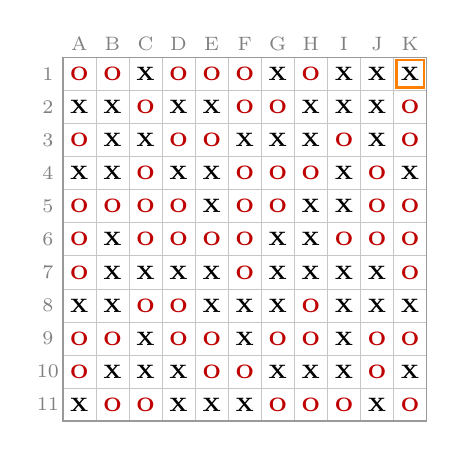
\begin{tikzpicture}[x=.42cm, y=.42cm]
\draw[gray!45, line width=.25pt] (0,0) -- (11,0);
\draw[gray!45, line width=.25pt] (0,0) -- (0,-11);
\draw[gray!45, line width=.25pt] (0,-1) -- (11,-1);
\draw[gray!45, line width=.25pt] (1,0) -- (1,-11);
\draw[gray!45, line width=.25pt] (0,-2) -- (11,-2);
\draw[gray!45, line width=.25pt] (2,0) -- (2,-11);
\draw[gray!45, line width=.25pt] (0,-3) -- (11,-3);
\draw[gray!45, line width=.25pt] (3,0) -- (3,-11);
\draw[gray!45, line width=.25pt] (0,-4) -- (11,-4);
\draw[gray!45, line width=.25pt] (4,0) -- (4,-11);
\draw[gray!45, line width=.25pt] (0,-5) -- (11,-5);
\draw[gray!45, line width=.25pt] (5,0) -- (5,-11);
\draw[gray!45, line width=.25pt] (0,-6) -- (11,-6);
\draw[gray!45, line width=.25pt] (6,0) -- (6,-11);
\draw[gray!45, line width=.25pt] (0,-7) -- (11,-7);
\draw[gray!45, line width=.25pt] (7,0) -- (7,-11);
\draw[gray!45, line width=.25pt] (0,-8) -- (11,-8);
\draw[gray!45, line width=.25pt] (8,0) -- (8,-11);
\draw[gray!45, line width=.25pt] (0,-9) -- (11,-9);
\draw[gray!45, line width=.25pt] (9,0) -- (9,-11);
\draw[gray!45, line width=.25pt] (0,-10) -- (11,-10);
\draw[gray!45, line width=.25pt] (10,0) -- (10,-11);
\draw[gray!45, line width=.25pt] (0,-11) -- (11,-11);
\draw[gray!45, line width=.25pt] (11,0) -- (11,-11);
\draw[gray!80, line width=.5pt] (0,0) rectangle (11,-11);
\node[font=\scriptsize, text=gray] at (0.5,.42) {A};
\node[font=\scriptsize, text=gray] at (1.5,.42) {B};
\node[font=\scriptsize, text=gray] at (2.5,.42) {C};
\node[font=\scriptsize, text=gray] at (3.5,.42) {D};
\node[font=\scriptsize, text=gray] at (4.5,.42) {E};
\node[font=\scriptsize, text=gray] at (5.5,.42) {F};
\node[font=\scriptsize, text=gray] at (6.5,.42) {G};
\node[font=\scriptsize, text=gray] at (7.5,.42) {H};
\node[font=\scriptsize, text=gray] at (8.5,.42) {I};
\node[font=\scriptsize, text=gray] at (9.5,.42) {J};
\node[font=\scriptsize, text=gray] at (10.5,.42) {K};
\node[font=\scriptsize, text=gray] at (-.45,-0.5) {1};
\node[font=\scriptsize, text=gray] at (-.45,-1.5) {2};
\node[font=\scriptsize, text=gray] at (-.45,-2.5) {3};
\node[font=\scriptsize, text=gray] at (-.45,-3.5) {4};
\node[font=\scriptsize, text=gray] at (-.45,-4.5) {5};
\node[font=\scriptsize, text=gray] at (-.45,-5.5) {6};
\node[font=\scriptsize, text=gray] at (-.45,-6.5) {7};
\node[font=\scriptsize, text=gray] at (-.45,-7.5) {8};
\node[font=\scriptsize, text=gray] at (-.45,-8.5) {9};
\node[font=\scriptsize, text=gray] at (-.45,-9.5) {10};
\node[font=\scriptsize, text=gray] at (-.45,-10.5) {11};
\node[text=red!75!black, font=\bfseries\scriptsize] at (0.5,-0.5) {O};
\node[text=red!75!black, font=\bfseries\scriptsize] at (1.5,-0.5) {O};
\node[text=black, font=\bfseries\scriptsize] at (2.5,-0.5) {X};
\node[text=red!75!black, font=\bfseries\scriptsize] at (3.5,-0.5) {O};
\node[text=red!75!black, font=\bfseries\scriptsize] at (4.5,-0.5) {O};
\node[text=red!75!black, font=\bfseries\scriptsize] at (5.5,-0.5) {O};
\node[text=black, font=\bfseries\scriptsize] at (6.5,-0.5) {X};
\node[text=red!75!black, font=\bfseries\scriptsize] at (7.5,-0.5) {O};
\node[text=black, font=\bfseries\scriptsize] at (8.5,-0.5) {X};
\node[text=black, font=\bfseries\scriptsize] at (9.5,-0.5) {X};
\node[text=black, font=\bfseries\scriptsize] at (10.5,-0.5) {X};
\draw[orange, line width=1pt] (10.08,-0.08) rectangle ++(.84,-.84);
\node[text=black, font=\bfseries\scriptsize] at (0.5,-1.5) {X};
\node[text=black, font=\bfseries\scriptsize] at (1.5,-1.5) {X};
\node[text=red!75!black, font=\bfseries\scriptsize] at (2.5,-1.5) {O};
\node[text=black, font=\bfseries\scriptsize] at (3.5,-1.5) {X};
\node[text=black, font=\bfseries\scriptsize] at (4.5,-1.5) {X};
\node[text=red!75!black, font=\bfseries\scriptsize] at (5.5,-1.5) {O};
\node[text=red!75!black, font=\bfseries\scriptsize] at (6.5,-1.5) {O};
\node[text=black, font=\bfseries\scriptsize] at (7.5,-1.5) {X};
\node[text=black, font=\bfseries\scriptsize] at (8.5,-1.5) {X};
\node[text=black, font=\bfseries\scriptsize] at (9.5,-1.5) {X};
\node[text=red!75!black, font=\bfseries\scriptsize] at (10.5,-1.5) {O};
\node[text=red!75!black, font=\bfseries\scriptsize] at (0.5,-2.5) {O};
\node[text=black, font=\bfseries\scriptsize] at (1.5,-2.5) {X};
\node[text=black, font=\bfseries\scriptsize] at (2.5,-2.5) {X};
\node[text=red!75!black, font=\bfseries\scriptsize] at (3.5,-2.5) {O};
\node[text=red!75!black, font=\bfseries\scriptsize] at (4.5,-2.5) {O};
\node[text=black, font=\bfseries\scriptsize] at (5.5,-2.5) {X};
\node[text=black, font=\bfseries\scriptsize] at (6.5,-2.5) {X};
\node[text=black, font=\bfseries\scriptsize] at (7.5,-2.5) {X};
\node[text=red!75!black, font=\bfseries\scriptsize] at (8.5,-2.5) {O};
\node[text=black, font=\bfseries\scriptsize] at (9.5,-2.5) {X};
\node[text=red!75!black, font=\bfseries\scriptsize] at (10.5,-2.5) {O};
\node[text=black, font=\bfseries\scriptsize] at (0.5,-3.5) {X};
\node[text=black, font=\bfseries\scriptsize] at (1.5,-3.5) {X};
\node[text=red!75!black, font=\bfseries\scriptsize] at (2.5,-3.5) {O};
\node[text=black, font=\bfseries\scriptsize] at (3.5,-3.5) {X};
\node[text=black, font=\bfseries\scriptsize] at (4.5,-3.5) {X};
\node[text=red!75!black, font=\bfseries\scriptsize] at (5.5,-3.5) {O};
\node[text=red!75!black, font=\bfseries\scriptsize] at (6.5,-3.5) {O};
\node[text=red!75!black, font=\bfseries\scriptsize] at (7.5,-3.5) {O};
\node[text=black, font=\bfseries\scriptsize] at (8.5,-3.5) {X};
\node[text=red!75!black, font=\bfseries\scriptsize] at (9.5,-3.5) {O};
\node[text=black, font=\bfseries\scriptsize] at (10.5,-3.5) {X};
\node[text=red!75!black, font=\bfseries\scriptsize] at (0.5,-4.5) {O};
\node[text=red!75!black, font=\bfseries\scriptsize] at (1.5,-4.5) {O};
\node[text=red!75!black, font=\bfseries\scriptsize] at (2.5,-4.5) {O};
\node[text=red!75!black, font=\bfseries\scriptsize] at (3.5,-4.5) {O};
\node[text=black, font=\bfseries\scriptsize] at (4.5,-4.5) {X};
\node[text=red!75!black, font=\bfseries\scriptsize] at (5.5,-4.5) {O};
\node[text=red!75!black, font=\bfseries\scriptsize] at (6.5,-4.5) {O};
\node[text=black, font=\bfseries\scriptsize] at (7.5,-4.5) {X};
\node[text=black, font=\bfseries\scriptsize] at (8.5,-4.5) {X};
\node[text=red!75!black, font=\bfseries\scriptsize] at (9.5,-4.5) {O};
\node[text=red!75!black, font=\bfseries\scriptsize] at (10.5,-4.5) {O};
\node[text=red!75!black, font=\bfseries\scriptsize] at (0.5,-5.5) {O};
\node[text=black, font=\bfseries\scriptsize] at (1.5,-5.5) {X};
\node[text=red!75!black, font=\bfseries\scriptsize] at (2.5,-5.5) {O};
\node[text=red!75!black, font=\bfseries\scriptsize] at (3.5,-5.5) {O};
\node[text=red!75!black, font=\bfseries\scriptsize] at (4.5,-5.5) {O};
\node[text=red!75!black, font=\bfseries\scriptsize] at (5.5,-5.5) {O};
\node[text=black, font=\bfseries\scriptsize] at (6.5,-5.5) {X};
\node[text=black, font=\bfseries\scriptsize] at (7.5,-5.5) {X};
\node[text=red!75!black, font=\bfseries\scriptsize] at (8.5,-5.5) {O};
\node[text=red!75!black, font=\bfseries\scriptsize] at (9.5,-5.5) {O};
\node[text=red!75!black, font=\bfseries\scriptsize] at (10.5,-5.5) {O};
\node[text=red!75!black, font=\bfseries\scriptsize] at (0.5,-6.5) {O};
\node[text=black, font=\bfseries\scriptsize] at (1.5,-6.5) {X};
\node[text=black, font=\bfseries\scriptsize] at (2.5,-6.5) {X};
\node[text=black, font=\bfseries\scriptsize] at (3.5,-6.5) {X};
\node[text=black, font=\bfseries\scriptsize] at (4.5,-6.5) {X};
\node[text=red!75!black, font=\bfseries\scriptsize] at (5.5,-6.5) {O};
\node[text=black, font=\bfseries\scriptsize] at (6.5,-6.5) {X};
\node[text=black, font=\bfseries\scriptsize] at (7.5,-6.5) {X};
\node[text=black, font=\bfseries\scriptsize] at (8.5,-6.5) {X};
\node[text=black, font=\bfseries\scriptsize] at (9.5,-6.5) {X};
\node[text=red!75!black, font=\bfseries\scriptsize] at (10.5,-6.5) {O};
\node[text=black, font=\bfseries\scriptsize] at (0.5,-7.5) {X};
\node[text=black, font=\bfseries\scriptsize] at (1.5,-7.5) {X};
\node[text=red!75!black, font=\bfseries\scriptsize] at (2.5,-7.5) {O};
\node[text=red!75!black, font=\bfseries\scriptsize] at (3.5,-7.5) {O};
\node[text=black, font=\bfseries\scriptsize] at (4.5,-7.5) {X};
\node[text=black, font=\bfseries\scriptsize] at (5.5,-7.5) {X};
\node[text=black, font=\bfseries\scriptsize] at (6.5,-7.5) {X};
\node[text=red!75!black, font=\bfseries\scriptsize] at (7.5,-7.5) {O};
\node[text=black, font=\bfseries\scriptsize] at (8.5,-7.5) {X};
\node[text=black, font=\bfseries\scriptsize] at (9.5,-7.5) {X};
\node[text=black, font=\bfseries\scriptsize] at (10.5,-7.5) {X};
\node[text=red!75!black, font=\bfseries\scriptsize] at (0.5,-8.5) {O};
\node[text=red!75!black, font=\bfseries\scriptsize] at (1.5,-8.5) {O};
\node[text=black, font=\bfseries\scriptsize] at (2.5,-8.5) {X};
\node[text=red!75!black, font=\bfseries\scriptsize] at (3.5,-8.5) {O};
\node[text=red!75!black, font=\bfseries\scriptsize] at (4.5,-8.5) {O};
\node[text=black, font=\bfseries\scriptsize] at (5.5,-8.5) {X};
\node[text=red!75!black, font=\bfseries\scriptsize] at (6.5,-8.5) {O};
\node[text=red!75!black, font=\bfseries\scriptsize] at (7.5,-8.5) {O};
\node[text=black, font=\bfseries\scriptsize] at (8.5,-8.5) {X};
\node[text=red!75!black, font=\bfseries\scriptsize] at (9.5,-8.5) {O};
\node[text=red!75!black, font=\bfseries\scriptsize] at (10.5,-8.5) {O};
\node[text=red!75!black, font=\bfseries\scriptsize] at (0.5,-9.5) {O};
\node[text=black, font=\bfseries\scriptsize] at (1.5,-9.5) {X};
\node[text=black, font=\bfseries\scriptsize] at (2.5,-9.5) {X};
\node[text=black, font=\bfseries\scriptsize] at (3.5,-9.5) {X};
\node[text=red!75!black, font=\bfseries\scriptsize] at (4.5,-9.5) {O};
\node[text=red!75!black, font=\bfseries\scriptsize] at (5.5,-9.5) {O};
\node[text=black, font=\bfseries\scriptsize] at (6.5,-9.5) {X};
\node[text=black, font=\bfseries\scriptsize] at (7.5,-9.5) {X};
\node[text=black, font=\bfseries\scriptsize] at (8.5,-9.5) {X};
\node[text=red!75!black, font=\bfseries\scriptsize] at (9.5,-9.5) {O};
\node[text=black, font=\bfseries\scriptsize] at (10.5,-9.5) {X};
\node[text=black, font=\bfseries\scriptsize] at (0.5,-10.5) {X};
\node[text=red!75!black, font=\bfseries\scriptsize] at (1.5,-10.5) {O};
\node[text=red!75!black, font=\bfseries\scriptsize] at (2.5,-10.5) {O};
\node[text=black, font=\bfseries\scriptsize] at (3.5,-10.5) {X};
\node[text=black, font=\bfseries\scriptsize] at (4.5,-10.5) {X};
\node[text=black, font=\bfseries\scriptsize] at (5.5,-10.5) {X};
\node[text=red!75!black, font=\bfseries\scriptsize] at (6.5,-10.5) {O};
\node[text=red!75!black, font=\bfseries\scriptsize] at (7.5,-10.5) {O};
\node[text=red!75!black, font=\bfseries\scriptsize] at (8.5,-10.5) {O};
\node[text=black, font=\bfseries\scriptsize] at (9.5,-10.5) {X};
\node[text=red!75!black, font=\bfseries\scriptsize] at (10.5,-10.5) {O};
\end{tikzpicture}
\end{center}
\paragraph{Cơ chế kết thúc} Bàn đầy mà không bên nào có năm quân liên tiếp; kết quả là hoà.
\paragraph{Nhận xét} Một trong số ít ván hoà giữa L7 và L8, kéo dài đủ 121 nước. Bàn đầy mà không bên nào có năm quân. Ván hoà hiếm vì cả hai tác tử đều có 200 mô phỏng và đủ mạnh để trừng phạt sai lầm; khi cả hai phòng thủ đúng, bàn có thể đầy. Đây là lý do điểm không nên chỉ báo thắng/thua; hoà là kết quả có thật và cần được tính nửa điểm.
\paragraph{Diễn biến} {\footnotesize 1.G6 2.G5 3.H5 4.F7 5.H6 6.F6 7.H7 8.H4 9.E7 10.F5 11.F8 12.F4 13.F3 14.G4 15.E4 16.E6 17.H3 18.D5 19.G8 20.C4 21.B3 22.I3 23.J2 24.J4 25.I4 26.H8 27.G7 28.C5 29.E5 30.C8 31.D7 32.C6 33.C7 34.D6 35.B6 36.E9 37.F9 38.I6 39.G10 40.G9 41.C3 42.D3 43.D2 44.F10 45.I7 46.B5 47.E2 48.G2 49.B2 50.C2 51.J7 52.K7 53.I8 54.H9 55.G3 56.J9 57.I9 58.E1 59.D4 60.A1 61.E8 62.H11 63.D11 64.E10 65.J3 66.K2 67.D10 68.D9 69.I10 70.I11 71.B7 72.A7 73.B10 74.G11 75.F11 76.B9 77.C9 78.D8 79.E11 80.A5 81.J11 82.A6 83.A4 84.D1 85.C1 86.K5 87.G1 88.K6 89.K4 90.B11 91.K10 92.J10 93.A8 94.K9 95.K8 96.K11 97.J8 98.J6 99.H10 100.C11 101.C10 102.J5 103.I5 104.K3 105.B8 106.A10 107.A11 108.A9 109.B4 110.E3 111.I2 112.A3 113.A2 114.F2 115.H2 116.B1 117.I1 118.F1 119.J1 120.H1 121.K1\par}

\subsection{E3 · L4 tự đấu · ván 311}
Khai cuộc gồm 3 nước: G7 → H4 → E6. X: \texttt{L4-MCTS}, O: \texttt{L4-MCTS}. Kết quả: O thắng sau 14 nước.
\begin{center}\small
\begin{tabular}{@{}rccll@{}}
\toprule
Ply & Màu & Nước & Nhận xét & Ô liên quan \\
\midrule
13 & X & F5 & Bỏ chặn duy nhất & G3 \\
14 & O & G3 & Thắng ngay & — \\
\bottomrule
\end{tabular}
\end{center}
\paragraph{Thế cờ trước nước quyết định (sau nước 13)}
\begin{center}
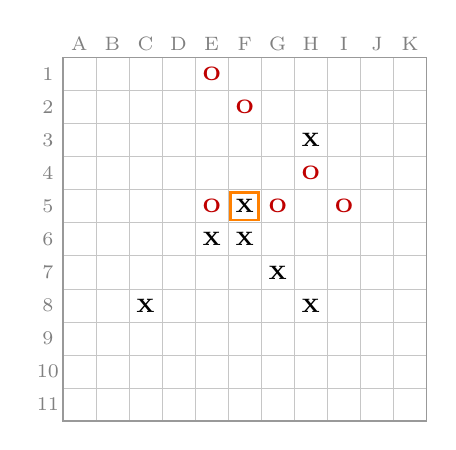
\begin{tikzpicture}[x=.42cm, y=.42cm]
\draw[gray!45, line width=.25pt] (0,0) -- (11,0);
\draw[gray!45, line width=.25pt] (0,0) -- (0,-11);
\draw[gray!45, line width=.25pt] (0,-1) -- (11,-1);
\draw[gray!45, line width=.25pt] (1,0) -- (1,-11);
\draw[gray!45, line width=.25pt] (0,-2) -- (11,-2);
\draw[gray!45, line width=.25pt] (2,0) -- (2,-11);
\draw[gray!45, line width=.25pt] (0,-3) -- (11,-3);
\draw[gray!45, line width=.25pt] (3,0) -- (3,-11);
\draw[gray!45, line width=.25pt] (0,-4) -- (11,-4);
\draw[gray!45, line width=.25pt] (4,0) -- (4,-11);
\draw[gray!45, line width=.25pt] (0,-5) -- (11,-5);
\draw[gray!45, line width=.25pt] (5,0) -- (5,-11);
\draw[gray!45, line width=.25pt] (0,-6) -- (11,-6);
\draw[gray!45, line width=.25pt] (6,0) -- (6,-11);
\draw[gray!45, line width=.25pt] (0,-7) -- (11,-7);
\draw[gray!45, line width=.25pt] (7,0) -- (7,-11);
\draw[gray!45, line width=.25pt] (0,-8) -- (11,-8);
\draw[gray!45, line width=.25pt] (8,0) -- (8,-11);
\draw[gray!45, line width=.25pt] (0,-9) -- (11,-9);
\draw[gray!45, line width=.25pt] (9,0) -- (9,-11);
\draw[gray!45, line width=.25pt] (0,-10) -- (11,-10);
\draw[gray!45, line width=.25pt] (10,0) -- (10,-11);
\draw[gray!45, line width=.25pt] (0,-11) -- (11,-11);
\draw[gray!45, line width=.25pt] (11,0) -- (11,-11);
\draw[gray!80, line width=.5pt] (0,0) rectangle (11,-11);
\node[font=\scriptsize, text=gray] at (0.5,.42) {A};
\node[font=\scriptsize, text=gray] at (1.5,.42) {B};
\node[font=\scriptsize, text=gray] at (2.5,.42) {C};
\node[font=\scriptsize, text=gray] at (3.5,.42) {D};
\node[font=\scriptsize, text=gray] at (4.5,.42) {E};
\node[font=\scriptsize, text=gray] at (5.5,.42) {F};
\node[font=\scriptsize, text=gray] at (6.5,.42) {G};
\node[font=\scriptsize, text=gray] at (7.5,.42) {H};
\node[font=\scriptsize, text=gray] at (8.5,.42) {I};
\node[font=\scriptsize, text=gray] at (9.5,.42) {J};
\node[font=\scriptsize, text=gray] at (10.5,.42) {K};
\node[font=\scriptsize, text=gray] at (-.45,-0.5) {1};
\node[font=\scriptsize, text=gray] at (-.45,-1.5) {2};
\node[font=\scriptsize, text=gray] at (-.45,-2.5) {3};
\node[font=\scriptsize, text=gray] at (-.45,-3.5) {4};
\node[font=\scriptsize, text=gray] at (-.45,-4.5) {5};
\node[font=\scriptsize, text=gray] at (-.45,-5.5) {6};
\node[font=\scriptsize, text=gray] at (-.45,-6.5) {7};
\node[font=\scriptsize, text=gray] at (-.45,-7.5) {8};
\node[font=\scriptsize, text=gray] at (-.45,-8.5) {9};
\node[font=\scriptsize, text=gray] at (-.45,-9.5) {10};
\node[font=\scriptsize, text=gray] at (-.45,-10.5) {11};
\node[text=red!75!black, font=\bfseries\scriptsize] at (4.5,-0.5) {O};
\node[text=red!75!black, font=\bfseries\scriptsize] at (5.5,-1.5) {O};
\node[text=black, font=\bfseries\scriptsize] at (7.5,-2.5) {X};
\node[text=red!75!black, font=\bfseries\scriptsize] at (7.5,-3.5) {O};
\node[text=red!75!black, font=\bfseries\scriptsize] at (4.5,-4.5) {O};
\node[text=black, font=\bfseries\scriptsize] at (5.5,-4.5) {X};
\draw[orange, line width=1pt] (5.08,-4.08) rectangle ++(.84,-.84);
\node[text=red!75!black, font=\bfseries\scriptsize] at (6.5,-4.5) {O};
\node[text=red!75!black, font=\bfseries\scriptsize] at (8.5,-4.5) {O};
\node[text=black, font=\bfseries\scriptsize] at (4.5,-5.5) {X};
\node[text=black, font=\bfseries\scriptsize] at (5.5,-5.5) {X};
\node[text=black, font=\bfseries\scriptsize] at (6.5,-6.5) {X};
\node[text=black, font=\bfseries\scriptsize] at (2.5,-7.5) {X};
\node[text=black, font=\bfseries\scriptsize] at (7.5,-7.5) {X};
\end{tikzpicture}
\end{center}
\paragraph{Thế kết thúc}
\begin{center}
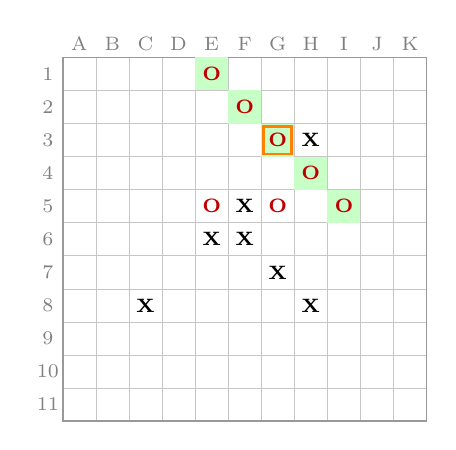
\begin{tikzpicture}[x=.42cm, y=.42cm]
\draw[gray!45, line width=.25pt] (0,0) -- (11,0);
\draw[gray!45, line width=.25pt] (0,0) -- (0,-11);
\draw[gray!45, line width=.25pt] (0,-1) -- (11,-1);
\draw[gray!45, line width=.25pt] (1,0) -- (1,-11);
\draw[gray!45, line width=.25pt] (0,-2) -- (11,-2);
\draw[gray!45, line width=.25pt] (2,0) -- (2,-11);
\draw[gray!45, line width=.25pt] (0,-3) -- (11,-3);
\draw[gray!45, line width=.25pt] (3,0) -- (3,-11);
\draw[gray!45, line width=.25pt] (0,-4) -- (11,-4);
\draw[gray!45, line width=.25pt] (4,0) -- (4,-11);
\draw[gray!45, line width=.25pt] (0,-5) -- (11,-5);
\draw[gray!45, line width=.25pt] (5,0) -- (5,-11);
\draw[gray!45, line width=.25pt] (0,-6) -- (11,-6);
\draw[gray!45, line width=.25pt] (6,0) -- (6,-11);
\draw[gray!45, line width=.25pt] (0,-7) -- (11,-7);
\draw[gray!45, line width=.25pt] (7,0) -- (7,-11);
\draw[gray!45, line width=.25pt] (0,-8) -- (11,-8);
\draw[gray!45, line width=.25pt] (8,0) -- (8,-11);
\draw[gray!45, line width=.25pt] (0,-9) -- (11,-9);
\draw[gray!45, line width=.25pt] (9,0) -- (9,-11);
\draw[gray!45, line width=.25pt] (0,-10) -- (11,-10);
\draw[gray!45, line width=.25pt] (10,0) -- (10,-11);
\draw[gray!45, line width=.25pt] (0,-11) -- (11,-11);
\draw[gray!45, line width=.25pt] (11,0) -- (11,-11);
\draw[gray!80, line width=.5pt] (0,0) rectangle (11,-11);
\node[font=\scriptsize, text=gray] at (0.5,.42) {A};
\node[font=\scriptsize, text=gray] at (1.5,.42) {B};
\node[font=\scriptsize, text=gray] at (2.5,.42) {C};
\node[font=\scriptsize, text=gray] at (3.5,.42) {D};
\node[font=\scriptsize, text=gray] at (4.5,.42) {E};
\node[font=\scriptsize, text=gray] at (5.5,.42) {F};
\node[font=\scriptsize, text=gray] at (6.5,.42) {G};
\node[font=\scriptsize, text=gray] at (7.5,.42) {H};
\node[font=\scriptsize, text=gray] at (8.5,.42) {I};
\node[font=\scriptsize, text=gray] at (9.5,.42) {J};
\node[font=\scriptsize, text=gray] at (10.5,.42) {K};
\node[font=\scriptsize, text=gray] at (-.45,-0.5) {1};
\node[font=\scriptsize, text=gray] at (-.45,-1.5) {2};
\node[font=\scriptsize, text=gray] at (-.45,-2.5) {3};
\node[font=\scriptsize, text=gray] at (-.45,-3.5) {4};
\node[font=\scriptsize, text=gray] at (-.45,-4.5) {5};
\node[font=\scriptsize, text=gray] at (-.45,-5.5) {6};
\node[font=\scriptsize, text=gray] at (-.45,-6.5) {7};
\node[font=\scriptsize, text=gray] at (-.45,-7.5) {8};
\node[font=\scriptsize, text=gray] at (-.45,-8.5) {9};
\node[font=\scriptsize, text=gray] at (-.45,-9.5) {10};
\node[font=\scriptsize, text=gray] at (-.45,-10.5) {11};
\fill[green!22] (4,0) rectangle ++(1,-1);
\node[text=red!75!black, font=\bfseries\scriptsize] at (4.5,-0.5) {O};
\fill[green!22] (5,-1) rectangle ++(1,-1);
\node[text=red!75!black, font=\bfseries\scriptsize] at (5.5,-1.5) {O};
\fill[green!22] (6,-2) rectangle ++(1,-1);
\node[text=red!75!black, font=\bfseries\scriptsize] at (6.5,-2.5) {O};
\draw[orange, line width=1pt] (6.08,-2.08) rectangle ++(.84,-.84);
\node[text=black, font=\bfseries\scriptsize] at (7.5,-2.5) {X};
\fill[green!22] (7,-3) rectangle ++(1,-1);
\node[text=red!75!black, font=\bfseries\scriptsize] at (7.5,-3.5) {O};
\node[text=red!75!black, font=\bfseries\scriptsize] at (4.5,-4.5) {O};
\node[text=black, font=\bfseries\scriptsize] at (5.5,-4.5) {X};
\node[text=red!75!black, font=\bfseries\scriptsize] at (6.5,-4.5) {O};
\fill[green!22] (8,-4) rectangle ++(1,-1);
\node[text=red!75!black, font=\bfseries\scriptsize] at (8.5,-4.5) {O};
\node[text=black, font=\bfseries\scriptsize] at (4.5,-5.5) {X};
\node[text=black, font=\bfseries\scriptsize] at (5.5,-5.5) {X};
\node[text=black, font=\bfseries\scriptsize] at (6.5,-6.5) {X};
\node[text=black, font=\bfseries\scriptsize] at (2.5,-7.5) {X};
\node[text=black, font=\bfseries\scriptsize] at (7.5,-7.5) {X};
\end{tikzpicture}
\end{center}
\paragraph{Cơ chế kết thúc} Trước nước áp chót, bên thắng có đúng một ô thắng ngay (G3); đối thủ không chặn, nên nước G3 hoàn thành dãy.
\paragraph{Nhận xét} L4 tự đấu, bên O thắng trong 14 nước bằng đường chéo E1–I5. Ở nước 13, bên X bỏ chặn một ô thắng duy nhất; bên O đi vào và thắng. Ván này cô đọng điểm yếu của MCTS rollout ngẫu nhiên: nó không có tri thức bắt buộc, nên trong tự đấu vẫn bỏ chặn. Đây là lý do L4 tự đấu cân bằng 50–50 nhưng tuyệt đối không có nghĩa là L4 mạnh.
\paragraph{Diễn biến} {\footnotesize 1.G7 2.H4 3.E6 4.F2 5.F6 6.E5 7.C8 8.G5 9.H3 10.I5 11.H8 12.E1 13.F5 14.G3\par}

\subsection{E3 · L5 tự đấu · ván 24}
Khai cuộc gồm 2 nước: E4 → G5. X: \texttt{L5-PolicySL}, O: \texttt{L5-PolicySL}. Kết quả: X thắng sau 27 nước.
\begin{center}\small
\begin{tabular}{@{}rccll@{}}
\toprule
Ply & Màu & Nước & Nhận xét & Ô liên quan \\
\midrule
16 & O & A7 & Chặn bắt buộc & A7 \\
22 & O & E6 & Chặn bắt buộc & E6 \\
24 & O & I9 & Đã ở thế buộc thua & — \\
25 & X & K11 & Bỏ lỡ thắng ngay & D3, D8 \\
26 & O & J11 & Đã ở thế buộc thua & — \\
27 & X & D8 & Thắng ngay & — \\
\bottomrule
\end{tabular}
\end{center}
\paragraph{Thế cờ trước nước quyết định (sau nước 26)}
\begin{center}
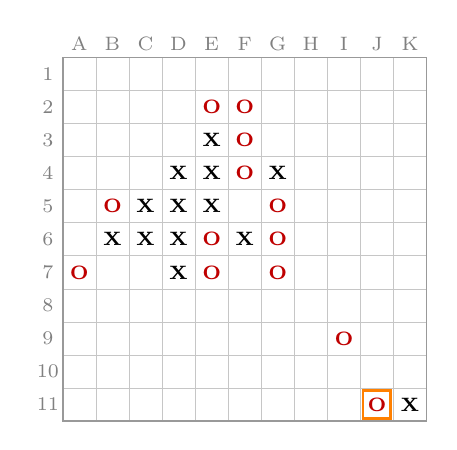
\begin{tikzpicture}[x=.42cm, y=.42cm]
\draw[gray!45, line width=.25pt] (0,0) -- (11,0);
\draw[gray!45, line width=.25pt] (0,0) -- (0,-11);
\draw[gray!45, line width=.25pt] (0,-1) -- (11,-1);
\draw[gray!45, line width=.25pt] (1,0) -- (1,-11);
\draw[gray!45, line width=.25pt] (0,-2) -- (11,-2);
\draw[gray!45, line width=.25pt] (2,0) -- (2,-11);
\draw[gray!45, line width=.25pt] (0,-3) -- (11,-3);
\draw[gray!45, line width=.25pt] (3,0) -- (3,-11);
\draw[gray!45, line width=.25pt] (0,-4) -- (11,-4);
\draw[gray!45, line width=.25pt] (4,0) -- (4,-11);
\draw[gray!45, line width=.25pt] (0,-5) -- (11,-5);
\draw[gray!45, line width=.25pt] (5,0) -- (5,-11);
\draw[gray!45, line width=.25pt] (0,-6) -- (11,-6);
\draw[gray!45, line width=.25pt] (6,0) -- (6,-11);
\draw[gray!45, line width=.25pt] (0,-7) -- (11,-7);
\draw[gray!45, line width=.25pt] (7,0) -- (7,-11);
\draw[gray!45, line width=.25pt] (0,-8) -- (11,-8);
\draw[gray!45, line width=.25pt] (8,0) -- (8,-11);
\draw[gray!45, line width=.25pt] (0,-9) -- (11,-9);
\draw[gray!45, line width=.25pt] (9,0) -- (9,-11);
\draw[gray!45, line width=.25pt] (0,-10) -- (11,-10);
\draw[gray!45, line width=.25pt] (10,0) -- (10,-11);
\draw[gray!45, line width=.25pt] (0,-11) -- (11,-11);
\draw[gray!45, line width=.25pt] (11,0) -- (11,-11);
\draw[gray!80, line width=.5pt] (0,0) rectangle (11,-11);
\node[font=\scriptsize, text=gray] at (0.5,.42) {A};
\node[font=\scriptsize, text=gray] at (1.5,.42) {B};
\node[font=\scriptsize, text=gray] at (2.5,.42) {C};
\node[font=\scriptsize, text=gray] at (3.5,.42) {D};
\node[font=\scriptsize, text=gray] at (4.5,.42) {E};
\node[font=\scriptsize, text=gray] at (5.5,.42) {F};
\node[font=\scriptsize, text=gray] at (6.5,.42) {G};
\node[font=\scriptsize, text=gray] at (7.5,.42) {H};
\node[font=\scriptsize, text=gray] at (8.5,.42) {I};
\node[font=\scriptsize, text=gray] at (9.5,.42) {J};
\node[font=\scriptsize, text=gray] at (10.5,.42) {K};
\node[font=\scriptsize, text=gray] at (-.45,-0.5) {1};
\node[font=\scriptsize, text=gray] at (-.45,-1.5) {2};
\node[font=\scriptsize, text=gray] at (-.45,-2.5) {3};
\node[font=\scriptsize, text=gray] at (-.45,-3.5) {4};
\node[font=\scriptsize, text=gray] at (-.45,-4.5) {5};
\node[font=\scriptsize, text=gray] at (-.45,-5.5) {6};
\node[font=\scriptsize, text=gray] at (-.45,-6.5) {7};
\node[font=\scriptsize, text=gray] at (-.45,-7.5) {8};
\node[font=\scriptsize, text=gray] at (-.45,-8.5) {9};
\node[font=\scriptsize, text=gray] at (-.45,-9.5) {10};
\node[font=\scriptsize, text=gray] at (-.45,-10.5) {11};
\node[text=red!75!black, font=\bfseries\scriptsize] at (4.5,-1.5) {O};
\node[text=red!75!black, font=\bfseries\scriptsize] at (5.5,-1.5) {O};
\node[text=black, font=\bfseries\scriptsize] at (4.5,-2.5) {X};
\node[text=red!75!black, font=\bfseries\scriptsize] at (5.5,-2.5) {O};
\node[text=black, font=\bfseries\scriptsize] at (3.5,-3.5) {X};
\node[text=black, font=\bfseries\scriptsize] at (4.5,-3.5) {X};
\node[text=red!75!black, font=\bfseries\scriptsize] at (5.5,-3.5) {O};
\node[text=black, font=\bfseries\scriptsize] at (6.5,-3.5) {X};
\node[text=red!75!black, font=\bfseries\scriptsize] at (1.5,-4.5) {O};
\node[text=black, font=\bfseries\scriptsize] at (2.5,-4.5) {X};
\node[text=black, font=\bfseries\scriptsize] at (3.5,-4.5) {X};
\node[text=black, font=\bfseries\scriptsize] at (4.5,-4.5) {X};
\node[text=red!75!black, font=\bfseries\scriptsize] at (6.5,-4.5) {O};
\node[text=black, font=\bfseries\scriptsize] at (1.5,-5.5) {X};
\node[text=black, font=\bfseries\scriptsize] at (2.5,-5.5) {X};
\node[text=black, font=\bfseries\scriptsize] at (3.5,-5.5) {X};
\node[text=red!75!black, font=\bfseries\scriptsize] at (4.5,-5.5) {O};
\node[text=black, font=\bfseries\scriptsize] at (5.5,-5.5) {X};
\node[text=red!75!black, font=\bfseries\scriptsize] at (6.5,-5.5) {O};
\node[text=red!75!black, font=\bfseries\scriptsize] at (0.5,-6.5) {O};
\node[text=black, font=\bfseries\scriptsize] at (3.5,-6.5) {X};
\node[text=red!75!black, font=\bfseries\scriptsize] at (4.5,-6.5) {O};
\node[text=red!75!black, font=\bfseries\scriptsize] at (6.5,-6.5) {O};
\node[text=red!75!black, font=\bfseries\scriptsize] at (8.5,-8.5) {O};
\node[text=red!75!black, font=\bfseries\scriptsize] at (9.5,-10.5) {O};
\draw[orange, line width=1pt] (9.08,-10.08) rectangle ++(.84,-.84);
\node[text=black, font=\bfseries\scriptsize] at (10.5,-10.5) {X};
\end{tikzpicture}
\end{center}
\paragraph{Thế kết thúc}
\begin{center}
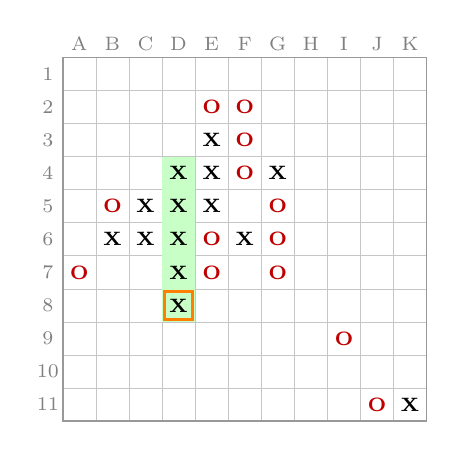
\begin{tikzpicture}[x=.42cm, y=.42cm]
\draw[gray!45, line width=.25pt] (0,0) -- (11,0);
\draw[gray!45, line width=.25pt] (0,0) -- (0,-11);
\draw[gray!45, line width=.25pt] (0,-1) -- (11,-1);
\draw[gray!45, line width=.25pt] (1,0) -- (1,-11);
\draw[gray!45, line width=.25pt] (0,-2) -- (11,-2);
\draw[gray!45, line width=.25pt] (2,0) -- (2,-11);
\draw[gray!45, line width=.25pt] (0,-3) -- (11,-3);
\draw[gray!45, line width=.25pt] (3,0) -- (3,-11);
\draw[gray!45, line width=.25pt] (0,-4) -- (11,-4);
\draw[gray!45, line width=.25pt] (4,0) -- (4,-11);
\draw[gray!45, line width=.25pt] (0,-5) -- (11,-5);
\draw[gray!45, line width=.25pt] (5,0) -- (5,-11);
\draw[gray!45, line width=.25pt] (0,-6) -- (11,-6);
\draw[gray!45, line width=.25pt] (6,0) -- (6,-11);
\draw[gray!45, line width=.25pt] (0,-7) -- (11,-7);
\draw[gray!45, line width=.25pt] (7,0) -- (7,-11);
\draw[gray!45, line width=.25pt] (0,-8) -- (11,-8);
\draw[gray!45, line width=.25pt] (8,0) -- (8,-11);
\draw[gray!45, line width=.25pt] (0,-9) -- (11,-9);
\draw[gray!45, line width=.25pt] (9,0) -- (9,-11);
\draw[gray!45, line width=.25pt] (0,-10) -- (11,-10);
\draw[gray!45, line width=.25pt] (10,0) -- (10,-11);
\draw[gray!45, line width=.25pt] (0,-11) -- (11,-11);
\draw[gray!45, line width=.25pt] (11,0) -- (11,-11);
\draw[gray!80, line width=.5pt] (0,0) rectangle (11,-11);
\node[font=\scriptsize, text=gray] at (0.5,.42) {A};
\node[font=\scriptsize, text=gray] at (1.5,.42) {B};
\node[font=\scriptsize, text=gray] at (2.5,.42) {C};
\node[font=\scriptsize, text=gray] at (3.5,.42) {D};
\node[font=\scriptsize, text=gray] at (4.5,.42) {E};
\node[font=\scriptsize, text=gray] at (5.5,.42) {F};
\node[font=\scriptsize, text=gray] at (6.5,.42) {G};
\node[font=\scriptsize, text=gray] at (7.5,.42) {H};
\node[font=\scriptsize, text=gray] at (8.5,.42) {I};
\node[font=\scriptsize, text=gray] at (9.5,.42) {J};
\node[font=\scriptsize, text=gray] at (10.5,.42) {K};
\node[font=\scriptsize, text=gray] at (-.45,-0.5) {1};
\node[font=\scriptsize, text=gray] at (-.45,-1.5) {2};
\node[font=\scriptsize, text=gray] at (-.45,-2.5) {3};
\node[font=\scriptsize, text=gray] at (-.45,-3.5) {4};
\node[font=\scriptsize, text=gray] at (-.45,-4.5) {5};
\node[font=\scriptsize, text=gray] at (-.45,-5.5) {6};
\node[font=\scriptsize, text=gray] at (-.45,-6.5) {7};
\node[font=\scriptsize, text=gray] at (-.45,-7.5) {8};
\node[font=\scriptsize, text=gray] at (-.45,-8.5) {9};
\node[font=\scriptsize, text=gray] at (-.45,-9.5) {10};
\node[font=\scriptsize, text=gray] at (-.45,-10.5) {11};
\node[text=red!75!black, font=\bfseries\scriptsize] at (4.5,-1.5) {O};
\node[text=red!75!black, font=\bfseries\scriptsize] at (5.5,-1.5) {O};
\node[text=black, font=\bfseries\scriptsize] at (4.5,-2.5) {X};
\node[text=red!75!black, font=\bfseries\scriptsize] at (5.5,-2.5) {O};
\fill[green!22] (3,-3) rectangle ++(1,-1);
\node[text=black, font=\bfseries\scriptsize] at (3.5,-3.5) {X};
\node[text=black, font=\bfseries\scriptsize] at (4.5,-3.5) {X};
\node[text=red!75!black, font=\bfseries\scriptsize] at (5.5,-3.5) {O};
\node[text=black, font=\bfseries\scriptsize] at (6.5,-3.5) {X};
\node[text=red!75!black, font=\bfseries\scriptsize] at (1.5,-4.5) {O};
\node[text=black, font=\bfseries\scriptsize] at (2.5,-4.5) {X};
\fill[green!22] (3,-4) rectangle ++(1,-1);
\node[text=black, font=\bfseries\scriptsize] at (3.5,-4.5) {X};
\node[text=black, font=\bfseries\scriptsize] at (4.5,-4.5) {X};
\node[text=red!75!black, font=\bfseries\scriptsize] at (6.5,-4.5) {O};
\node[text=black, font=\bfseries\scriptsize] at (1.5,-5.5) {X};
\node[text=black, font=\bfseries\scriptsize] at (2.5,-5.5) {X};
\fill[green!22] (3,-5) rectangle ++(1,-1);
\node[text=black, font=\bfseries\scriptsize] at (3.5,-5.5) {X};
\node[text=red!75!black, font=\bfseries\scriptsize] at (4.5,-5.5) {O};
\node[text=black, font=\bfseries\scriptsize] at (5.5,-5.5) {X};
\node[text=red!75!black, font=\bfseries\scriptsize] at (6.5,-5.5) {O};
\node[text=red!75!black, font=\bfseries\scriptsize] at (0.5,-6.5) {O};
\fill[green!22] (3,-6) rectangle ++(1,-1);
\node[text=black, font=\bfseries\scriptsize] at (3.5,-6.5) {X};
\node[text=red!75!black, font=\bfseries\scriptsize] at (4.5,-6.5) {O};
\node[text=red!75!black, font=\bfseries\scriptsize] at (6.5,-6.5) {O};
\fill[green!22] (3,-7) rectangle ++(1,-1);
\node[text=black, font=\bfseries\scriptsize] at (3.5,-7.5) {X};
\draw[orange, line width=1pt] (3.08,-7.08) rectangle ++(.84,-.84);
\node[text=red!75!black, font=\bfseries\scriptsize] at (8.5,-8.5) {O};
\node[text=red!75!black, font=\bfseries\scriptsize] at (9.5,-10.5) {O};
\node[text=black, font=\bfseries\scriptsize] at (10.5,-10.5) {X};
\end{tikzpicture}
\end{center}
\paragraph{Cơ chế kết thúc} Trước nước áp chót, bên thắng đã có 2 ô thắng ngay (D3, D8); đối thủ chỉ chặn được một ô, nên nước D8 hoàn thành dãy năm quân.
\paragraph{Nhận xét} L5 tự đấu, bên X thắng trong 27 nước bằng cột D (D4–D8). Bên X bỏ lỡ một nước thắng ngay ở nước 25 nhưng vẫn thắng sau đó. Ván minh hoạ policy-only có thể sai ở nước quyết định mà không bị trừng phạt nếu đối thủ cũng là chính nó. Trong đấu với tác tử mạnh hơn, cùng lỗi đó thường bị trừng phạt ngay.
\paragraph{Diễn biến} {\footnotesize 1.E4 2.G5 3.E5 4.E7 5.F6 6.G7 7.D4 8.G6 9.G4 10.F4 11.E3 12.E2 13.C5 14.F2 15.B6 16.A7 17.D5 18.B5 19.C6 20.F3 21.D6 22.E6 23.D7 24.I9 25.K11 26.J11 27.D8\par}

\subsection{E3 · L7 tự đấu · ván 232}
Khai cuộc gồm 2 nước: H8 → G6. X: \texttt{L7-PUCT}, O: \texttt{L7-PUCT}. Kết quả: O thắng sau 28 nước.
\begin{center}\small
\begin{tabular}{@{}rccll@{}}
\toprule
Ply & Màu & Nước & Nhận xét & Ô liên quan \\
\midrule
15 & X & F10 & Chặn bắt buộc & F10 \\
19 & X & D10 & Chặn bắt buộc & D10 \\
21 & X & G3 & Chặn bắt buộc & G3 \\
24 & O & K8 & Chặn bắt buộc & K8 \\
27 & X & F2 & Bỏ chặn duy nhất & E6 \\
28 & O & E6 & Thắng ngay & — \\
\bottomrule
\end{tabular}
\end{center}
\paragraph{Thế cờ trước nước quyết định (sau nước 27)}
\begin{center}
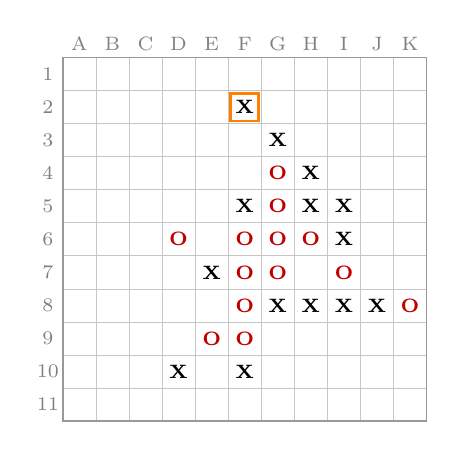
\begin{tikzpicture}[x=.42cm, y=.42cm]
\draw[gray!45, line width=.25pt] (0,0) -- (11,0);
\draw[gray!45, line width=.25pt] (0,0) -- (0,-11);
\draw[gray!45, line width=.25pt] (0,-1) -- (11,-1);
\draw[gray!45, line width=.25pt] (1,0) -- (1,-11);
\draw[gray!45, line width=.25pt] (0,-2) -- (11,-2);
\draw[gray!45, line width=.25pt] (2,0) -- (2,-11);
\draw[gray!45, line width=.25pt] (0,-3) -- (11,-3);
\draw[gray!45, line width=.25pt] (3,0) -- (3,-11);
\draw[gray!45, line width=.25pt] (0,-4) -- (11,-4);
\draw[gray!45, line width=.25pt] (4,0) -- (4,-11);
\draw[gray!45, line width=.25pt] (0,-5) -- (11,-5);
\draw[gray!45, line width=.25pt] (5,0) -- (5,-11);
\draw[gray!45, line width=.25pt] (0,-6) -- (11,-6);
\draw[gray!45, line width=.25pt] (6,0) -- (6,-11);
\draw[gray!45, line width=.25pt] (0,-7) -- (11,-7);
\draw[gray!45, line width=.25pt] (7,0) -- (7,-11);
\draw[gray!45, line width=.25pt] (0,-8) -- (11,-8);
\draw[gray!45, line width=.25pt] (8,0) -- (8,-11);
\draw[gray!45, line width=.25pt] (0,-9) -- (11,-9);
\draw[gray!45, line width=.25pt] (9,0) -- (9,-11);
\draw[gray!45, line width=.25pt] (0,-10) -- (11,-10);
\draw[gray!45, line width=.25pt] (10,0) -- (10,-11);
\draw[gray!45, line width=.25pt] (0,-11) -- (11,-11);
\draw[gray!45, line width=.25pt] (11,0) -- (11,-11);
\draw[gray!80, line width=.5pt] (0,0) rectangle (11,-11);
\node[font=\scriptsize, text=gray] at (0.5,.42) {A};
\node[font=\scriptsize, text=gray] at (1.5,.42) {B};
\node[font=\scriptsize, text=gray] at (2.5,.42) {C};
\node[font=\scriptsize, text=gray] at (3.5,.42) {D};
\node[font=\scriptsize, text=gray] at (4.5,.42) {E};
\node[font=\scriptsize, text=gray] at (5.5,.42) {F};
\node[font=\scriptsize, text=gray] at (6.5,.42) {G};
\node[font=\scriptsize, text=gray] at (7.5,.42) {H};
\node[font=\scriptsize, text=gray] at (8.5,.42) {I};
\node[font=\scriptsize, text=gray] at (9.5,.42) {J};
\node[font=\scriptsize, text=gray] at (10.5,.42) {K};
\node[font=\scriptsize, text=gray] at (-.45,-0.5) {1};
\node[font=\scriptsize, text=gray] at (-.45,-1.5) {2};
\node[font=\scriptsize, text=gray] at (-.45,-2.5) {3};
\node[font=\scriptsize, text=gray] at (-.45,-3.5) {4};
\node[font=\scriptsize, text=gray] at (-.45,-4.5) {5};
\node[font=\scriptsize, text=gray] at (-.45,-5.5) {6};
\node[font=\scriptsize, text=gray] at (-.45,-6.5) {7};
\node[font=\scriptsize, text=gray] at (-.45,-7.5) {8};
\node[font=\scriptsize, text=gray] at (-.45,-8.5) {9};
\node[font=\scriptsize, text=gray] at (-.45,-9.5) {10};
\node[font=\scriptsize, text=gray] at (-.45,-10.5) {11};
\node[text=black, font=\bfseries\scriptsize] at (5.5,-1.5) {X};
\draw[orange, line width=1pt] (5.08,-1.08) rectangle ++(.84,-.84);
\node[text=black, font=\bfseries\scriptsize] at (6.5,-2.5) {X};
\node[text=red!75!black, font=\bfseries\scriptsize] at (6.5,-3.5) {O};
\node[text=black, font=\bfseries\scriptsize] at (7.5,-3.5) {X};
\node[text=black, font=\bfseries\scriptsize] at (5.5,-4.5) {X};
\node[text=red!75!black, font=\bfseries\scriptsize] at (6.5,-4.5) {O};
\node[text=black, font=\bfseries\scriptsize] at (7.5,-4.5) {X};
\node[text=black, font=\bfseries\scriptsize] at (8.5,-4.5) {X};
\node[text=red!75!black, font=\bfseries\scriptsize] at (3.5,-5.5) {O};
\node[text=red!75!black, font=\bfseries\scriptsize] at (5.5,-5.5) {O};
\node[text=red!75!black, font=\bfseries\scriptsize] at (6.5,-5.5) {O};
\node[text=red!75!black, font=\bfseries\scriptsize] at (7.5,-5.5) {O};
\node[text=black, font=\bfseries\scriptsize] at (8.5,-5.5) {X};
\node[text=black, font=\bfseries\scriptsize] at (4.5,-6.5) {X};
\node[text=red!75!black, font=\bfseries\scriptsize] at (5.5,-6.5) {O};
\node[text=red!75!black, font=\bfseries\scriptsize] at (6.5,-6.5) {O};
\node[text=red!75!black, font=\bfseries\scriptsize] at (8.5,-6.5) {O};
\node[text=red!75!black, font=\bfseries\scriptsize] at (5.5,-7.5) {O};
\node[text=black, font=\bfseries\scriptsize] at (6.5,-7.5) {X};
\node[text=black, font=\bfseries\scriptsize] at (7.5,-7.5) {X};
\node[text=black, font=\bfseries\scriptsize] at (8.5,-7.5) {X};
\node[text=black, font=\bfseries\scriptsize] at (9.5,-7.5) {X};
\node[text=red!75!black, font=\bfseries\scriptsize] at (10.5,-7.5) {O};
\node[text=red!75!black, font=\bfseries\scriptsize] at (4.5,-8.5) {O};
\node[text=red!75!black, font=\bfseries\scriptsize] at (5.5,-8.5) {O};
\node[text=black, font=\bfseries\scriptsize] at (3.5,-9.5) {X};
\node[text=black, font=\bfseries\scriptsize] at (5.5,-9.5) {X};
\end{tikzpicture}
\end{center}
\paragraph{Thế kết thúc}
\begin{center}
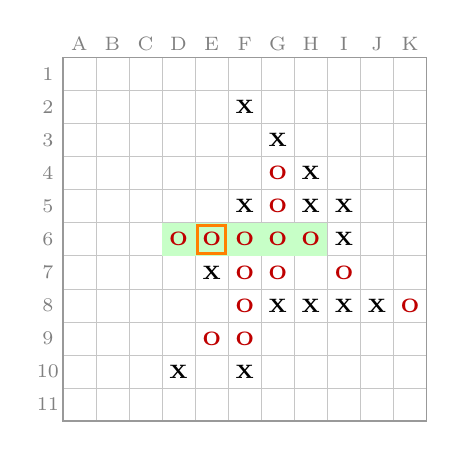
\begin{tikzpicture}[x=.42cm, y=.42cm]
\draw[gray!45, line width=.25pt] (0,0) -- (11,0);
\draw[gray!45, line width=.25pt] (0,0) -- (0,-11);
\draw[gray!45, line width=.25pt] (0,-1) -- (11,-1);
\draw[gray!45, line width=.25pt] (1,0) -- (1,-11);
\draw[gray!45, line width=.25pt] (0,-2) -- (11,-2);
\draw[gray!45, line width=.25pt] (2,0) -- (2,-11);
\draw[gray!45, line width=.25pt] (0,-3) -- (11,-3);
\draw[gray!45, line width=.25pt] (3,0) -- (3,-11);
\draw[gray!45, line width=.25pt] (0,-4) -- (11,-4);
\draw[gray!45, line width=.25pt] (4,0) -- (4,-11);
\draw[gray!45, line width=.25pt] (0,-5) -- (11,-5);
\draw[gray!45, line width=.25pt] (5,0) -- (5,-11);
\draw[gray!45, line width=.25pt] (0,-6) -- (11,-6);
\draw[gray!45, line width=.25pt] (6,0) -- (6,-11);
\draw[gray!45, line width=.25pt] (0,-7) -- (11,-7);
\draw[gray!45, line width=.25pt] (7,0) -- (7,-11);
\draw[gray!45, line width=.25pt] (0,-8) -- (11,-8);
\draw[gray!45, line width=.25pt] (8,0) -- (8,-11);
\draw[gray!45, line width=.25pt] (0,-9) -- (11,-9);
\draw[gray!45, line width=.25pt] (9,0) -- (9,-11);
\draw[gray!45, line width=.25pt] (0,-10) -- (11,-10);
\draw[gray!45, line width=.25pt] (10,0) -- (10,-11);
\draw[gray!45, line width=.25pt] (0,-11) -- (11,-11);
\draw[gray!45, line width=.25pt] (11,0) -- (11,-11);
\draw[gray!80, line width=.5pt] (0,0) rectangle (11,-11);
\node[font=\scriptsize, text=gray] at (0.5,.42) {A};
\node[font=\scriptsize, text=gray] at (1.5,.42) {B};
\node[font=\scriptsize, text=gray] at (2.5,.42) {C};
\node[font=\scriptsize, text=gray] at (3.5,.42) {D};
\node[font=\scriptsize, text=gray] at (4.5,.42) {E};
\node[font=\scriptsize, text=gray] at (5.5,.42) {F};
\node[font=\scriptsize, text=gray] at (6.5,.42) {G};
\node[font=\scriptsize, text=gray] at (7.5,.42) {H};
\node[font=\scriptsize, text=gray] at (8.5,.42) {I};
\node[font=\scriptsize, text=gray] at (9.5,.42) {J};
\node[font=\scriptsize, text=gray] at (10.5,.42) {K};
\node[font=\scriptsize, text=gray] at (-.45,-0.5) {1};
\node[font=\scriptsize, text=gray] at (-.45,-1.5) {2};
\node[font=\scriptsize, text=gray] at (-.45,-2.5) {3};
\node[font=\scriptsize, text=gray] at (-.45,-3.5) {4};
\node[font=\scriptsize, text=gray] at (-.45,-4.5) {5};
\node[font=\scriptsize, text=gray] at (-.45,-5.5) {6};
\node[font=\scriptsize, text=gray] at (-.45,-6.5) {7};
\node[font=\scriptsize, text=gray] at (-.45,-7.5) {8};
\node[font=\scriptsize, text=gray] at (-.45,-8.5) {9};
\node[font=\scriptsize, text=gray] at (-.45,-9.5) {10};
\node[font=\scriptsize, text=gray] at (-.45,-10.5) {11};
\node[text=black, font=\bfseries\scriptsize] at (5.5,-1.5) {X};
\node[text=black, font=\bfseries\scriptsize] at (6.5,-2.5) {X};
\node[text=red!75!black, font=\bfseries\scriptsize] at (6.5,-3.5) {O};
\node[text=black, font=\bfseries\scriptsize] at (7.5,-3.5) {X};
\node[text=black, font=\bfseries\scriptsize] at (5.5,-4.5) {X};
\node[text=red!75!black, font=\bfseries\scriptsize] at (6.5,-4.5) {O};
\node[text=black, font=\bfseries\scriptsize] at (7.5,-4.5) {X};
\node[text=black, font=\bfseries\scriptsize] at (8.5,-4.5) {X};
\fill[green!22] (3,-5) rectangle ++(1,-1);
\node[text=red!75!black, font=\bfseries\scriptsize] at (3.5,-5.5) {O};
\fill[green!22] (4,-5) rectangle ++(1,-1);
\node[text=red!75!black, font=\bfseries\scriptsize] at (4.5,-5.5) {O};
\draw[orange, line width=1pt] (4.08,-5.08) rectangle ++(.84,-.84);
\fill[green!22] (5,-5) rectangle ++(1,-1);
\node[text=red!75!black, font=\bfseries\scriptsize] at (5.5,-5.5) {O};
\fill[green!22] (6,-5) rectangle ++(1,-1);
\node[text=red!75!black, font=\bfseries\scriptsize] at (6.5,-5.5) {O};
\fill[green!22] (7,-5) rectangle ++(1,-1);
\node[text=red!75!black, font=\bfseries\scriptsize] at (7.5,-5.5) {O};
\node[text=black, font=\bfseries\scriptsize] at (8.5,-5.5) {X};
\node[text=black, font=\bfseries\scriptsize] at (4.5,-6.5) {X};
\node[text=red!75!black, font=\bfseries\scriptsize] at (5.5,-6.5) {O};
\node[text=red!75!black, font=\bfseries\scriptsize] at (6.5,-6.5) {O};
\node[text=red!75!black, font=\bfseries\scriptsize] at (8.5,-6.5) {O};
\node[text=red!75!black, font=\bfseries\scriptsize] at (5.5,-7.5) {O};
\node[text=black, font=\bfseries\scriptsize] at (6.5,-7.5) {X};
\node[text=black, font=\bfseries\scriptsize] at (7.5,-7.5) {X};
\node[text=black, font=\bfseries\scriptsize] at (8.5,-7.5) {X};
\node[text=black, font=\bfseries\scriptsize] at (9.5,-7.5) {X};
\node[text=red!75!black, font=\bfseries\scriptsize] at (10.5,-7.5) {O};
\node[text=red!75!black, font=\bfseries\scriptsize] at (4.5,-8.5) {O};
\node[text=red!75!black, font=\bfseries\scriptsize] at (5.5,-8.5) {O};
\node[text=black, font=\bfseries\scriptsize] at (3.5,-9.5) {X};
\node[text=black, font=\bfseries\scriptsize] at (5.5,-9.5) {X};
\end{tikzpicture}
\end{center}
\paragraph{Cơ chế kết thúc} Trước nước áp chót, bên thắng có đúng một ô thắng ngay (E6); đối thủ không chặn, nên nước E6 hoàn thành dãy.
\paragraph{Nhận xét} L7 tự đấu, bên O thắng trong 28 nước bằng hàng ngang D6–H6. Ở nước 27, bên X bỏ chặn một ô thắng duy nhất; bên O đi vào và thắng. Ngay cả PUCT với 200 mô phỏng vẫn có thể bỏ chặn trong tự đấu, dù tỷ lệ thấp hơn nhiều so với L4. Đây là bằng chứng định lượng rằng tìm kiếm giảm nhưng không xoá lỗi chiến thuật.
\paragraph{Diễn biến} {\footnotesize 1.H8 2.G6 3.G8 4.F7 5.I8 6.F8 7.H5 8.F6 9.F5 10.G5 11.E7 12.H6 13.I6 14.F9 15.F10 16.G7 17.I5 18.E9 19.D10 20.G4 21.G3 22.I7 23.J8 24.K8 25.H4 26.D6 27.F2 28.E6\par}

\subsection{E3 · L8 tự đấu · ván 370}
Khai cuộc gồm 3 nước: G5 → E8 → E6. X: \texttt{L8-AlphaZero}, O: \texttt{L8-AlphaZero}. Kết quả: X thắng sau 45 nước.
\begin{center}\small
\begin{tabular}{@{}rccll@{}}
\toprule
Ply & Màu & Nước & Nhận xét & Ô liên quan \\
\midrule
24 & O & C11 & Chặn bắt buộc & C11 \\
29 & X & H8 & Chặn bắt buộc & H8 \\
38 & O & B3 & Chặn bắt buộc & B3 \\
44 & O & I6 & Bỏ chặn duy nhất & D7 \\
45 & X & D7 & Thắng ngay & — \\
\bottomrule
\end{tabular}
\end{center}
\paragraph{Thế cờ trước nước quyết định (sau nước 44)}
\begin{center}
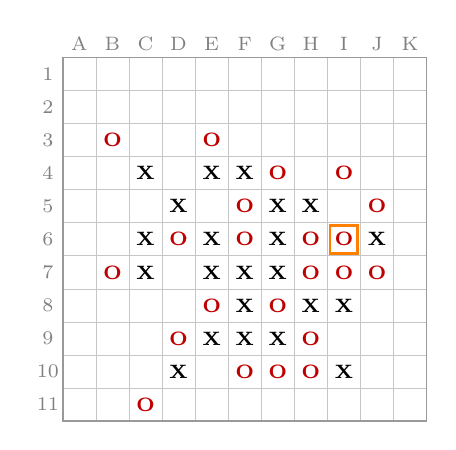
\begin{tikzpicture}[x=.42cm, y=.42cm]
\draw[gray!45, line width=.25pt] (0,0) -- (11,0);
\draw[gray!45, line width=.25pt] (0,0) -- (0,-11);
\draw[gray!45, line width=.25pt] (0,-1) -- (11,-1);
\draw[gray!45, line width=.25pt] (1,0) -- (1,-11);
\draw[gray!45, line width=.25pt] (0,-2) -- (11,-2);
\draw[gray!45, line width=.25pt] (2,0) -- (2,-11);
\draw[gray!45, line width=.25pt] (0,-3) -- (11,-3);
\draw[gray!45, line width=.25pt] (3,0) -- (3,-11);
\draw[gray!45, line width=.25pt] (0,-4) -- (11,-4);
\draw[gray!45, line width=.25pt] (4,0) -- (4,-11);
\draw[gray!45, line width=.25pt] (0,-5) -- (11,-5);
\draw[gray!45, line width=.25pt] (5,0) -- (5,-11);
\draw[gray!45, line width=.25pt] (0,-6) -- (11,-6);
\draw[gray!45, line width=.25pt] (6,0) -- (6,-11);
\draw[gray!45, line width=.25pt] (0,-7) -- (11,-7);
\draw[gray!45, line width=.25pt] (7,0) -- (7,-11);
\draw[gray!45, line width=.25pt] (0,-8) -- (11,-8);
\draw[gray!45, line width=.25pt] (8,0) -- (8,-11);
\draw[gray!45, line width=.25pt] (0,-9) -- (11,-9);
\draw[gray!45, line width=.25pt] (9,0) -- (9,-11);
\draw[gray!45, line width=.25pt] (0,-10) -- (11,-10);
\draw[gray!45, line width=.25pt] (10,0) -- (10,-11);
\draw[gray!45, line width=.25pt] (0,-11) -- (11,-11);
\draw[gray!45, line width=.25pt] (11,0) -- (11,-11);
\draw[gray!80, line width=.5pt] (0,0) rectangle (11,-11);
\node[font=\scriptsize, text=gray] at (0.5,.42) {A};
\node[font=\scriptsize, text=gray] at (1.5,.42) {B};
\node[font=\scriptsize, text=gray] at (2.5,.42) {C};
\node[font=\scriptsize, text=gray] at (3.5,.42) {D};
\node[font=\scriptsize, text=gray] at (4.5,.42) {E};
\node[font=\scriptsize, text=gray] at (5.5,.42) {F};
\node[font=\scriptsize, text=gray] at (6.5,.42) {G};
\node[font=\scriptsize, text=gray] at (7.5,.42) {H};
\node[font=\scriptsize, text=gray] at (8.5,.42) {I};
\node[font=\scriptsize, text=gray] at (9.5,.42) {J};
\node[font=\scriptsize, text=gray] at (10.5,.42) {K};
\node[font=\scriptsize, text=gray] at (-.45,-0.5) {1};
\node[font=\scriptsize, text=gray] at (-.45,-1.5) {2};
\node[font=\scriptsize, text=gray] at (-.45,-2.5) {3};
\node[font=\scriptsize, text=gray] at (-.45,-3.5) {4};
\node[font=\scriptsize, text=gray] at (-.45,-4.5) {5};
\node[font=\scriptsize, text=gray] at (-.45,-5.5) {6};
\node[font=\scriptsize, text=gray] at (-.45,-6.5) {7};
\node[font=\scriptsize, text=gray] at (-.45,-7.5) {8};
\node[font=\scriptsize, text=gray] at (-.45,-8.5) {9};
\node[font=\scriptsize, text=gray] at (-.45,-9.5) {10};
\node[font=\scriptsize, text=gray] at (-.45,-10.5) {11};
\node[text=red!75!black, font=\bfseries\scriptsize] at (1.5,-2.5) {O};
\node[text=red!75!black, font=\bfseries\scriptsize] at (4.5,-2.5) {O};
\node[text=black, font=\bfseries\scriptsize] at (2.5,-3.5) {X};
\node[text=black, font=\bfseries\scriptsize] at (4.5,-3.5) {X};
\node[text=black, font=\bfseries\scriptsize] at (5.5,-3.5) {X};
\node[text=red!75!black, font=\bfseries\scriptsize] at (6.5,-3.5) {O};
\node[text=red!75!black, font=\bfseries\scriptsize] at (8.5,-3.5) {O};
\node[text=black, font=\bfseries\scriptsize] at (3.5,-4.5) {X};
\node[text=red!75!black, font=\bfseries\scriptsize] at (5.5,-4.5) {O};
\node[text=black, font=\bfseries\scriptsize] at (6.5,-4.5) {X};
\node[text=black, font=\bfseries\scriptsize] at (7.5,-4.5) {X};
\node[text=red!75!black, font=\bfseries\scriptsize] at (9.5,-4.5) {O};
\node[text=black, font=\bfseries\scriptsize] at (2.5,-5.5) {X};
\node[text=red!75!black, font=\bfseries\scriptsize] at (3.5,-5.5) {O};
\node[text=black, font=\bfseries\scriptsize] at (4.5,-5.5) {X};
\node[text=red!75!black, font=\bfseries\scriptsize] at (5.5,-5.5) {O};
\node[text=black, font=\bfseries\scriptsize] at (6.5,-5.5) {X};
\node[text=red!75!black, font=\bfseries\scriptsize] at (7.5,-5.5) {O};
\node[text=red!75!black, font=\bfseries\scriptsize] at (8.5,-5.5) {O};
\draw[orange, line width=1pt] (8.08,-5.08) rectangle ++(.84,-.84);
\node[text=black, font=\bfseries\scriptsize] at (9.5,-5.5) {X};
\node[text=red!75!black, font=\bfseries\scriptsize] at (1.5,-6.5) {O};
\node[text=black, font=\bfseries\scriptsize] at (2.5,-6.5) {X};
\node[text=black, font=\bfseries\scriptsize] at (4.5,-6.5) {X};
\node[text=black, font=\bfseries\scriptsize] at (5.5,-6.5) {X};
\node[text=black, font=\bfseries\scriptsize] at (6.5,-6.5) {X};
\node[text=red!75!black, font=\bfseries\scriptsize] at (7.5,-6.5) {O};
\node[text=red!75!black, font=\bfseries\scriptsize] at (8.5,-6.5) {O};
\node[text=red!75!black, font=\bfseries\scriptsize] at (9.5,-6.5) {O};
\node[text=red!75!black, font=\bfseries\scriptsize] at (4.5,-7.5) {O};
\node[text=black, font=\bfseries\scriptsize] at (5.5,-7.5) {X};
\node[text=red!75!black, font=\bfseries\scriptsize] at (6.5,-7.5) {O};
\node[text=black, font=\bfseries\scriptsize] at (7.5,-7.5) {X};
\node[text=black, font=\bfseries\scriptsize] at (8.5,-7.5) {X};
\node[text=red!75!black, font=\bfseries\scriptsize] at (3.5,-8.5) {O};
\node[text=black, font=\bfseries\scriptsize] at (4.5,-8.5) {X};
\node[text=black, font=\bfseries\scriptsize] at (5.5,-8.5) {X};
\node[text=black, font=\bfseries\scriptsize] at (6.5,-8.5) {X};
\node[text=red!75!black, font=\bfseries\scriptsize] at (7.5,-8.5) {O};
\node[text=black, font=\bfseries\scriptsize] at (3.5,-9.5) {X};
\node[text=red!75!black, font=\bfseries\scriptsize] at (5.5,-9.5) {O};
\node[text=red!75!black, font=\bfseries\scriptsize] at (6.5,-9.5) {O};
\node[text=red!75!black, font=\bfseries\scriptsize] at (7.5,-9.5) {O};
\node[text=black, font=\bfseries\scriptsize] at (8.5,-9.5) {X};
\node[text=red!75!black, font=\bfseries\scriptsize] at (2.5,-10.5) {O};
\end{tikzpicture}
\end{center}
\paragraph{Thế kết thúc}
\begin{center}
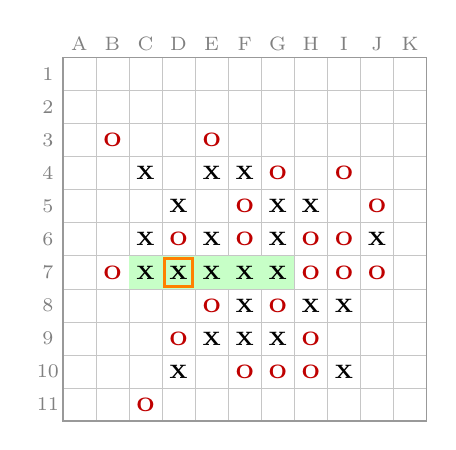
\begin{tikzpicture}[x=.42cm, y=.42cm]
\draw[gray!45, line width=.25pt] (0,0) -- (11,0);
\draw[gray!45, line width=.25pt] (0,0) -- (0,-11);
\draw[gray!45, line width=.25pt] (0,-1) -- (11,-1);
\draw[gray!45, line width=.25pt] (1,0) -- (1,-11);
\draw[gray!45, line width=.25pt] (0,-2) -- (11,-2);
\draw[gray!45, line width=.25pt] (2,0) -- (2,-11);
\draw[gray!45, line width=.25pt] (0,-3) -- (11,-3);
\draw[gray!45, line width=.25pt] (3,0) -- (3,-11);
\draw[gray!45, line width=.25pt] (0,-4) -- (11,-4);
\draw[gray!45, line width=.25pt] (4,0) -- (4,-11);
\draw[gray!45, line width=.25pt] (0,-5) -- (11,-5);
\draw[gray!45, line width=.25pt] (5,0) -- (5,-11);
\draw[gray!45, line width=.25pt] (0,-6) -- (11,-6);
\draw[gray!45, line width=.25pt] (6,0) -- (6,-11);
\draw[gray!45, line width=.25pt] (0,-7) -- (11,-7);
\draw[gray!45, line width=.25pt] (7,0) -- (7,-11);
\draw[gray!45, line width=.25pt] (0,-8) -- (11,-8);
\draw[gray!45, line width=.25pt] (8,0) -- (8,-11);
\draw[gray!45, line width=.25pt] (0,-9) -- (11,-9);
\draw[gray!45, line width=.25pt] (9,0) -- (9,-11);
\draw[gray!45, line width=.25pt] (0,-10) -- (11,-10);
\draw[gray!45, line width=.25pt] (10,0) -- (10,-11);
\draw[gray!45, line width=.25pt] (0,-11) -- (11,-11);
\draw[gray!45, line width=.25pt] (11,0) -- (11,-11);
\draw[gray!80, line width=.5pt] (0,0) rectangle (11,-11);
\node[font=\scriptsize, text=gray] at (0.5,.42) {A};
\node[font=\scriptsize, text=gray] at (1.5,.42) {B};
\node[font=\scriptsize, text=gray] at (2.5,.42) {C};
\node[font=\scriptsize, text=gray] at (3.5,.42) {D};
\node[font=\scriptsize, text=gray] at (4.5,.42) {E};
\node[font=\scriptsize, text=gray] at (5.5,.42) {F};
\node[font=\scriptsize, text=gray] at (6.5,.42) {G};
\node[font=\scriptsize, text=gray] at (7.5,.42) {H};
\node[font=\scriptsize, text=gray] at (8.5,.42) {I};
\node[font=\scriptsize, text=gray] at (9.5,.42) {J};
\node[font=\scriptsize, text=gray] at (10.5,.42) {K};
\node[font=\scriptsize, text=gray] at (-.45,-0.5) {1};
\node[font=\scriptsize, text=gray] at (-.45,-1.5) {2};
\node[font=\scriptsize, text=gray] at (-.45,-2.5) {3};
\node[font=\scriptsize, text=gray] at (-.45,-3.5) {4};
\node[font=\scriptsize, text=gray] at (-.45,-4.5) {5};
\node[font=\scriptsize, text=gray] at (-.45,-5.5) {6};
\node[font=\scriptsize, text=gray] at (-.45,-6.5) {7};
\node[font=\scriptsize, text=gray] at (-.45,-7.5) {8};
\node[font=\scriptsize, text=gray] at (-.45,-8.5) {9};
\node[font=\scriptsize, text=gray] at (-.45,-9.5) {10};
\node[font=\scriptsize, text=gray] at (-.45,-10.5) {11};
\node[text=red!75!black, font=\bfseries\scriptsize] at (1.5,-2.5) {O};
\node[text=red!75!black, font=\bfseries\scriptsize] at (4.5,-2.5) {O};
\node[text=black, font=\bfseries\scriptsize] at (2.5,-3.5) {X};
\node[text=black, font=\bfseries\scriptsize] at (4.5,-3.5) {X};
\node[text=black, font=\bfseries\scriptsize] at (5.5,-3.5) {X};
\node[text=red!75!black, font=\bfseries\scriptsize] at (6.5,-3.5) {O};
\node[text=red!75!black, font=\bfseries\scriptsize] at (8.5,-3.5) {O};
\node[text=black, font=\bfseries\scriptsize] at (3.5,-4.5) {X};
\node[text=red!75!black, font=\bfseries\scriptsize] at (5.5,-4.5) {O};
\node[text=black, font=\bfseries\scriptsize] at (6.5,-4.5) {X};
\node[text=black, font=\bfseries\scriptsize] at (7.5,-4.5) {X};
\node[text=red!75!black, font=\bfseries\scriptsize] at (9.5,-4.5) {O};
\node[text=black, font=\bfseries\scriptsize] at (2.5,-5.5) {X};
\node[text=red!75!black, font=\bfseries\scriptsize] at (3.5,-5.5) {O};
\node[text=black, font=\bfseries\scriptsize] at (4.5,-5.5) {X};
\node[text=red!75!black, font=\bfseries\scriptsize] at (5.5,-5.5) {O};
\node[text=black, font=\bfseries\scriptsize] at (6.5,-5.5) {X};
\node[text=red!75!black, font=\bfseries\scriptsize] at (7.5,-5.5) {O};
\node[text=red!75!black, font=\bfseries\scriptsize] at (8.5,-5.5) {O};
\node[text=black, font=\bfseries\scriptsize] at (9.5,-5.5) {X};
\node[text=red!75!black, font=\bfseries\scriptsize] at (1.5,-6.5) {O};
\fill[green!22] (2,-6) rectangle ++(1,-1);
\node[text=black, font=\bfseries\scriptsize] at (2.5,-6.5) {X};
\fill[green!22] (3,-6) rectangle ++(1,-1);
\node[text=black, font=\bfseries\scriptsize] at (3.5,-6.5) {X};
\draw[orange, line width=1pt] (3.08,-6.08) rectangle ++(.84,-.84);
\fill[green!22] (4,-6) rectangle ++(1,-1);
\node[text=black, font=\bfseries\scriptsize] at (4.5,-6.5) {X};
\fill[green!22] (5,-6) rectangle ++(1,-1);
\node[text=black, font=\bfseries\scriptsize] at (5.5,-6.5) {X};
\fill[green!22] (6,-6) rectangle ++(1,-1);
\node[text=black, font=\bfseries\scriptsize] at (6.5,-6.5) {X};
\node[text=red!75!black, font=\bfseries\scriptsize] at (7.5,-6.5) {O};
\node[text=red!75!black, font=\bfseries\scriptsize] at (8.5,-6.5) {O};
\node[text=red!75!black, font=\bfseries\scriptsize] at (9.5,-6.5) {O};
\node[text=red!75!black, font=\bfseries\scriptsize] at (4.5,-7.5) {O};
\node[text=black, font=\bfseries\scriptsize] at (5.5,-7.5) {X};
\node[text=red!75!black, font=\bfseries\scriptsize] at (6.5,-7.5) {O};
\node[text=black, font=\bfseries\scriptsize] at (7.5,-7.5) {X};
\node[text=black, font=\bfseries\scriptsize] at (8.5,-7.5) {X};
\node[text=red!75!black, font=\bfseries\scriptsize] at (3.5,-8.5) {O};
\node[text=black, font=\bfseries\scriptsize] at (4.5,-8.5) {X};
\node[text=black, font=\bfseries\scriptsize] at (5.5,-8.5) {X};
\node[text=black, font=\bfseries\scriptsize] at (6.5,-8.5) {X};
\node[text=red!75!black, font=\bfseries\scriptsize] at (7.5,-8.5) {O};
\node[text=black, font=\bfseries\scriptsize] at (3.5,-9.5) {X};
\node[text=red!75!black, font=\bfseries\scriptsize] at (5.5,-9.5) {O};
\node[text=red!75!black, font=\bfseries\scriptsize] at (6.5,-9.5) {O};
\node[text=red!75!black, font=\bfseries\scriptsize] at (7.5,-9.5) {O};
\node[text=black, font=\bfseries\scriptsize] at (8.5,-9.5) {X};
\node[text=red!75!black, font=\bfseries\scriptsize] at (2.5,-10.5) {O};
\end{tikzpicture}
\end{center}
\paragraph{Cơ chế kết thúc} Trước nước áp chót, bên thắng có đúng một ô thắng ngay (D7); đối thủ không chặn, nên nước D7 hoàn thành dãy.
\paragraph{Nhận xét} L8 tự đấu, bên X thắng trong 45 nước bằng hàng ngang C7–G7. Ở nước 44, bên O bỏ chặn một ô thắng duy nhất nhưng bên X không chuyển ngay thành thắng; đến nước 45 mới hoàn thành. Ván cho thấy ngay cả L8 cũng có lúc bỏ chặn, nhưng đối thủ không phải lúc nào cũng trừng phạt được. Đây là lý do phân tích lỗi phải đếm cả cơ hội và kết quả, không chỉ kết quả.
\paragraph{Diễn biến} {\footnotesize 1.G5 2.E8 3.E6 4.F5 5.G6 6.F6 7.G7 8.G8 9.F8 10.H6 11.E7 12.D6 13.F7 14.H7 15.H5 16.G4 17.F9 18.F10 19.E9 20.D9 21.G9 22.I4 23.D10 24.C11 25.F4 26.H10 27.D5 28.H9 29.H8 30.G10 31.I10 32.J7 33.I8 34.J5 35.J6 36.I7 37.C4 38.B3 39.E4 40.E3 41.C6 42.B7 43.C7 44.I6 45.D7\par}